\documentclass[a4paper, 12pt]{report}
\usepackage{graphicx} % Required for inserting images
\usepackage[T1]{fontenc}
\usepackage[latin1]{inputenc}
\usepackage{glossaries}
\usepackage{graphicx}
\usepackage{amsfonts}
\usepackage{subfigure}
\usepackage[hidelinks]{hyperref}
\usepackage{pifont}
\usepackage{array}
\usepackage{booktabs}
\usepackage{cleveref}
\usepackage{algorithm}
\usepackage{algpseudocode}
\usepackage{multicol}
\usepackage{eufrak}
\usepackage{amssymb}
\usepackage{listings}
\usepackage{amsthm}
\usepackage{verbatim}
\usepackage{tikz}
\usetikzlibrary{shapes,arrows}
\usepackage{tikz}
\tikzstyle{mybox} = [draw=black, thin, rectangle, rounded corners, inner ysep=5pt, inner xsep=5pt, fill=blue!15]
\newtheorem{theorem}{Teorema}
\usepackage[a4paper, top=2.8cm , bottom=2cm , right=2cm , left=2cm ]{geometry}

\usepackage[table,xcdraw]{xcolor}
\usepackage{array}
\usepackage{biblatex} %Imports biblatex package
\addbibresource{bibliography.bib} %Import the bibliography file
\usepackage{longtable}

\title{
    {\color{black}
    \textbf{  \Huge{MACHINE LEARNING FOR VISION AND MULTIMEDIA} }\\}
    \textit{Lecture notes}
    \linespread{2}
}
\author{Carlo Migliaccio}
\date{AA 2024/2025}

\theoremstyle{definition}
\newtheorem{definition}{Definition}[section]

\pagestyle{headings}

\theoremstyle{remark}
\newtheorem*{remark}{Remark}

\begin{document}
\maketitle
\tableofcontents

\chapter{Introduction}
Among the definitions one gives of \textbf{Machine learning} we can say that it is a \textit{"Field of study that gives computers the ability to learn without being explicitly programmed"}. Nowadays, the \textit{Artificial intelligence} is in general that the electricity was in the 19$^\text{th}$ century. Something of paramount importance! \\
There are several methodologies and subfields in Machine Learning and the distinction is based on \textit{how much and how} the human collaborate and of the type of provided data. The most important classification is the one between:
\begin{itemize}
    \itemsep-0.3em
    \item \textit{Supervised learning} (this course), is the approach which uses \textbf{a-priori knowledge} embedded in the data that are used for training algorithms and recognize patterns;
    \item \textit{Unsupervided learning}, is the approach at the opposite whose main feature is not using \textit{labeled data} for assess the tasks.
    \item \textit{Other approaches}. Due to its vastness, in machine learning you can find for sure other subfields. For example the \textit{Reinforcement learning, Semi-Supervised learning, trasnfer learning}. However they are all outside the purposes of this course. 
\end{itemize}

\begin{figure}[h]
    \centering
    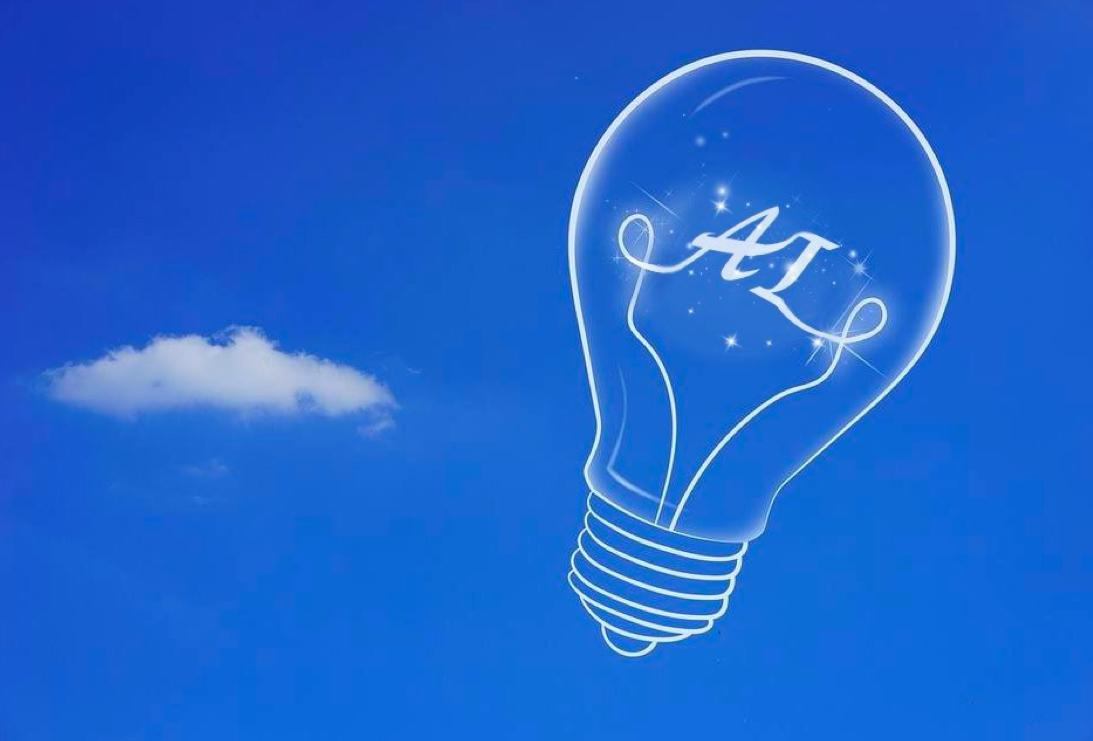
\includegraphics[scale=0.2]{img/AI.jpeg}
\end{figure}

\section{Supervised learning}
From \textsc{Wikipedia (EN)}: \textsf{Supervised learning (SL) is a paradigm in machine learning where input objects (for example, a vector of predictor variables) and a desired output value (also known as a human-labeled supervisory signal) train a model.} In the following we are giving some simple introductory examples about two among the most used techniques in supervised learning.
\subsection{Linear Regression}
Let us imagine we are supposed to create a model that allows us to \textbf{predict the price of an house}. For sake of simplicity and clarity, suppose that our \textit{dataset entries} have one feature (the house size in ft$^2$) and the \textit{price} which represents the \textbf{correct answers}.
Using this data we seek for a model which could predict, given the size of an unknown house, his price (in dollars, \$). Several choices can be made. At first, using either a linear or a nonlinear model and so on. It is remarkable that -- even in such a simple example -- we are facing a \textbf{supervised} problem since the right answers are given! This particular case is a problem of \textbf{regression} since we want to \textbf{predict a continuous valued output}, in our case the price.

\begin{figure}[h]
    \centering
    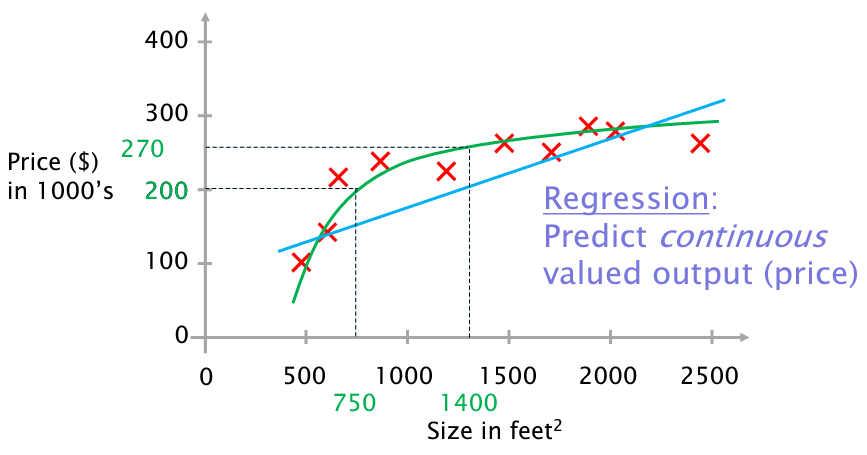
\includegraphics[scale=0.5]{img/prices.png}
\end{figure}

In the figure above is shown the example in which two different models are used, clearly the predicted values for an unknown record is different according to the chosen model.

\subsection{Classification}
On the other hand, when we want to predict a discrete value (eg. YES/NO), we have a \textbf{classification} problem. Again, let us consider a trivial example: we want to predict whether a tumor is malignant or not according to its size. Even in this case we have one feature for the data (\textit{tumor size}) and all the training data are labeled with the YES/NO answer.

\begin{figure}[h]
    \centering
    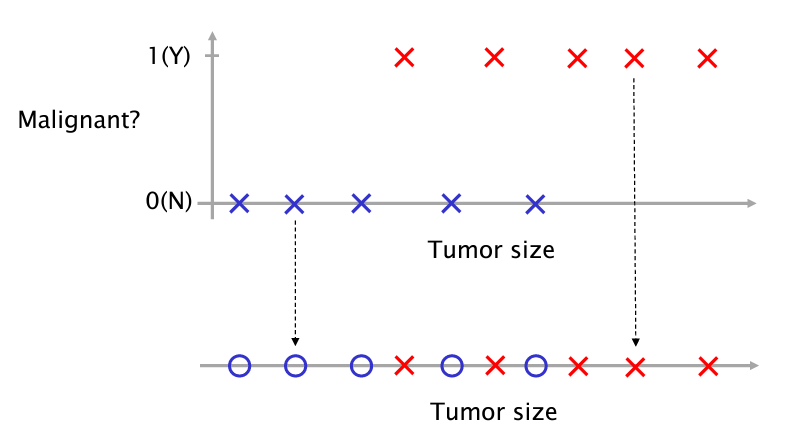
\includegraphics[scale=0.5]{img/tumor.png}
\end{figure}

The figure shows a graphical representation of the dataset. In this case since the answers are associated with different symbols, a more compact representation is given by a one-axis diagram: one feature is given, furthermore a different symbol is associated to different classes. Note that in this case we are in front of a a \textbf{binary classification problem}, in general the classes to predict are not necessarily in number of two. \\
This was just an example to understand and introduce the problem, but in real-world applications, one feature is not sufficient to build a good model! For sake of clarity, let us complicate a little bit the example we have just presented by adding a new feature associated with the \textit{age of the patient}.

\begin{figure}[h]
    \centering
    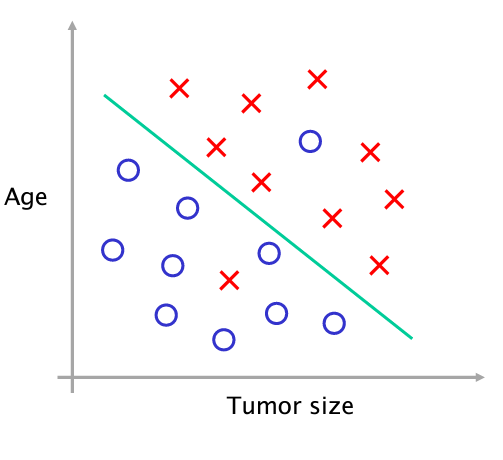
\includegraphics[scale=0.5]{img/tumor_more.png}
    \caption{Bi-variate problem with linear decision boundary}
\end{figure}

In this case the data set is represented in a 2D graph, one axis for each feature and a different symbol for each class. Now, given a record associated with a new patient, what is the class for its tumor? In this case can be useful to individuate a \textbf{decision boundary} according to which one can decide clearly what is the prediction (Positive/Negative). In the two parts there are some outliers, for this reason one can be tempted to build a more "accurate" decision boundary that perfectly split the two classes.

\begin{figure}[h]
    \centering
    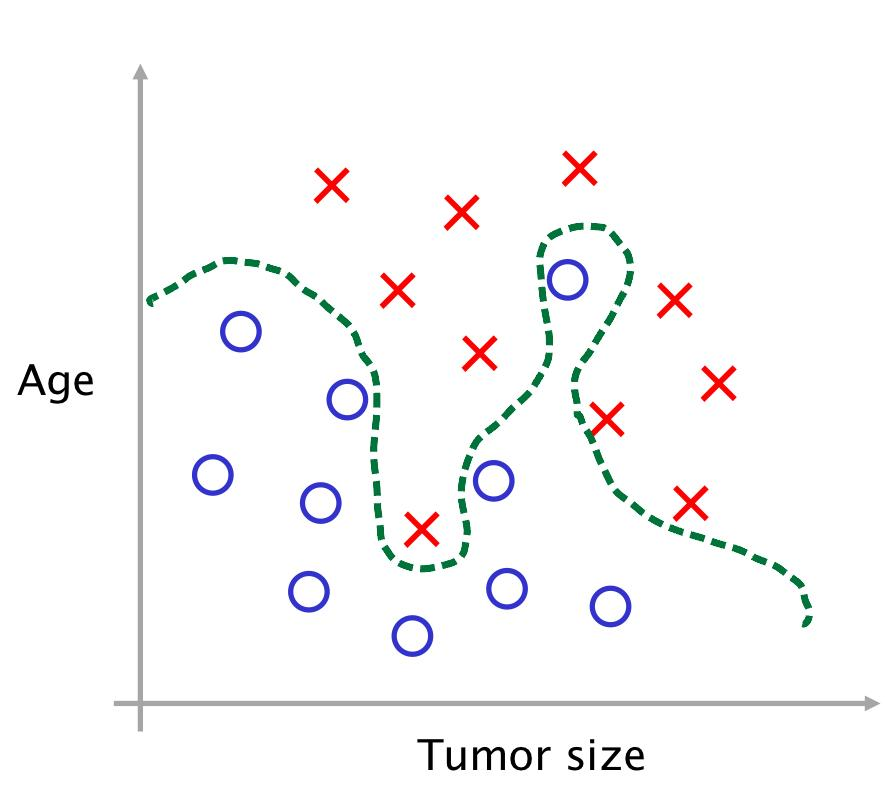
\includegraphics[scale=0.2]{img/overfit.jpeg}
    \caption{Example of overfitting}
\end{figure}

\noindent
Is this a good model for the given problem? NO! This model will have very bad \textit{performances of generalization} with new records to be classified, since it is too much related to the given dataset. In a colloquial way we say that: \textsf{The model has learnt the by heart the dataset}. A problem known as \textbf{overfitting}. \\
Finally, we can say that few features will result in a bad model, on the other hand also too much features will result in a bad model for another problem known as the \textbf{curse of dimensionality}.\footnote{
    In these case techniques of dimensionality reduction has to be employed.
}

\section{Unsupervided learning}
At the opposite of the \textit{supervised approach}, here patterns are learnt exclusively from unlabeled data. The most common example of such an approach is the \textbf{Clustering}.

\subsection{Clustering}
In this case several algorithms are employed to discover groups called \textbf{clusters} associated with objects which are similar in some sense. In general, very often distance-based measures are used to individuate the groups. One of the most famous clustering algorithm is the \textit{K-Mean}. The following figure is an example of bivariate clustered data. 

\begin{figure}[h]
    \centering
    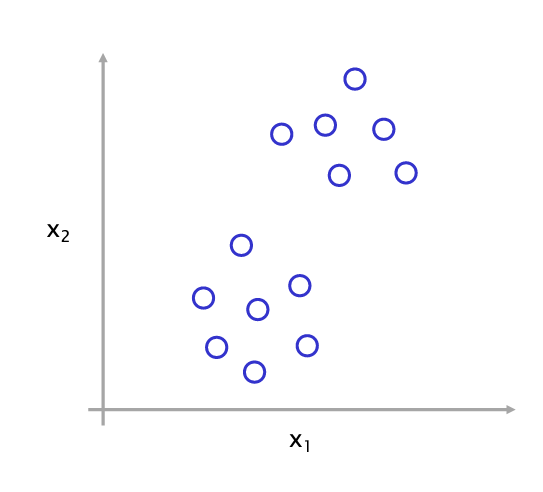
\includegraphics[scale=0.5]{img/clustering.png}
\end{figure}

Unsupervised techniques are used also in bioinformatics in manipulated \textit{DNA microarrays}, for gropuing together similar web pages, for analysis of astronomical data and so on.
Let us come back to the first example of \textit{price prediction} and formalize some aspects we have only mentioned. The objective here is to exploit this example to introduce and better clarify several concepts.\\
\section{Model representation}
At first, the training set we are using is something similar to the following:

\begin{table}[h]
    \centering
    \begin{tabular}{c c}
        \textbf{Size in feet$^2$($x$)}&\textbf{Price(\$) in 1000's($y$)}\\
        \hline
        2104&460\\
        1416&232\\
        1534&315\\
        852&178\\
        ...&...
    \end{tabular}
\end{table}
\noindent
We will indicate with $m$ the number of samples of the training set (number of rows), $x$ is the input (possibly multivariate) variable, $y$ is the output variable, $(x,y)$ indicates generically a sample from the training set, while $(x^{(i)}, y^{(i)})$ indicates the $i$-th sample of the training set.

\begin{figure}[h]
    \centering
    \label{}
    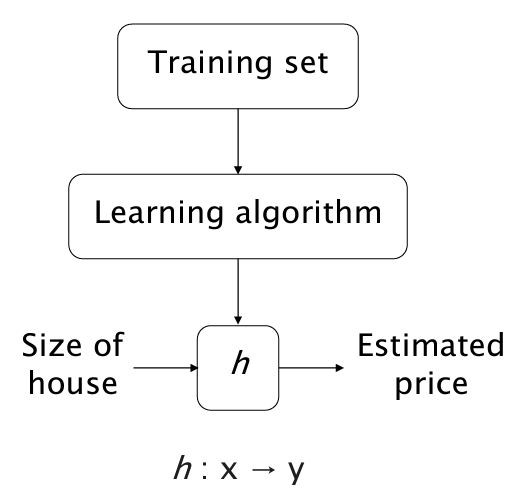
\includegraphics[scale=0.5]{img/model.png}
    \caption{Scheme for model construction (price prediction)}
\end{figure}

The figure above shows schematically the steps in order to produce a certain model for the analysed case-study. Very briefly, a \textbf{training set} is used by a \textbf{learning algorithm} to obtain an \textit{hypotesis} $h_\theta(x)$ which is later used for the prediction.\\
In the case we want to solve a \textbf{univariate linear regression problem} the hypotesis $h$ has got the shape:
\begin{equation}
    h_{\theta}(x)=\theta_0+\theta_1{x}
\end{equation}
where $\theta_0$ and $\theta_1$ are the parameters of the line.\footnote{
    We can imagine them as two handles to: move up/down the line ($\theta_0$) and to rotate it ($\theta_1$).
} We call \textit{univariate} the the problem since we have only one feature and it is a \textit{linear regression} because we want to predict the price (output) according to a line.\footnote{
    Note that in case of a \textbf{neural network} the parameters and the hypotesis assume a different notation. In particular the hypotesis becomes the \textit{predicted value} indicated with $\hat{y}$, the parameters are split in a \textbf{bias}, indicated with $b$ whose role is the one played by $\theta_0$, while the $\theta_i$, $i=1,...,n$ are the weights $w_i$
 }
\textbf{Question: How can we choose $\theta_0, \theta_1$?} Intuitively one can choose the parameters associated with the line $h_\theta(x)$ which is as closest as possible to the given $y$. Very often these parameters are the ones which solve the following problem: 
\begin{equation}\label{eq:ls1}
    \min_{\theta_0, \theta_1} {\frac{1}{m} \sum_{i=1}^{m}{
        \frac{1}{2} \bigl(
            \underbrace{h_\theta(x^{(i)})}_{\textsf{predicted value}}-
            \underbrace{y^{(i)}}_{\textsf{actual value}}
            \bigr)^2
    }}
\end{equation}
The function $\frac{1}{2} (
    h_\theta(x^{(i)})-y^{(i)})^2$ is the \textsf{Loss}($h_\theta(x), y$) or \textsf{Cost}($h_\theta(x),y$).  If we call $J(\theta_0, \theta_1)$ the argument of the minimization problem the (\ref{eq:ls1}), the problem to solve can be expressed as
\begin{equation}\label{ls2}
    \min_{\theta_0, \theta_1} {J({\theta_0, \theta_1})}
\end{equation}
Summarizing: we want to perform a prediction using the hypotesis $h$ which is dependent on parameters $\theta_0, \theta_1$ which are issued by minimizing a certain functional $J(\theta_0, \theta_1)$. Let us investigate better on the role of $J$ in this supervised learning task.\\
At first -- for sake of simplicity -- we can eliminate a degree of freedom fixing the parameter $\theta_0$ to be (without loss of generality) $\theta_0=0$. For each choice of $\theta_1$ we will obtain a $h_{\theta_1}(x)$. If we compute $J(\theta_1)$ (for each $\theta$) will obtain a certain univariate function $J(\theta_1)$, the minimization of which will give us the \textit{optimal} $\theta_1$ parameter for our hypotesis. An example is shown in the following figure:

\begin{figure}[h]
    \centering
    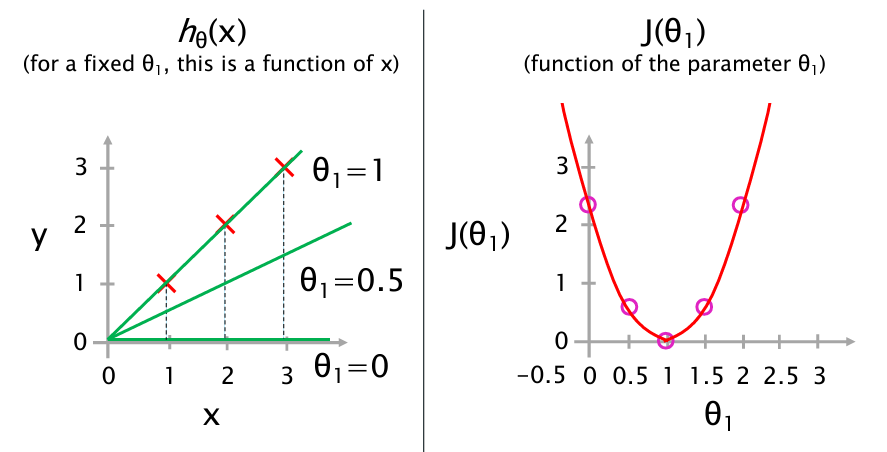
\includegraphics[scale=0.7]{img/J_univariate.png}
\end{figure}
\noindent
Analyzing the complete model, we have two degrees of freedom (DOF) since  $\theta_0, \theta_1$ can vary. In this case the functional to be minimized has to be represented in a 3D space, then we obtain a surface similar to one presented in the following figure:

\begin{figure}[h]\label{fig:surface}
   \centering
   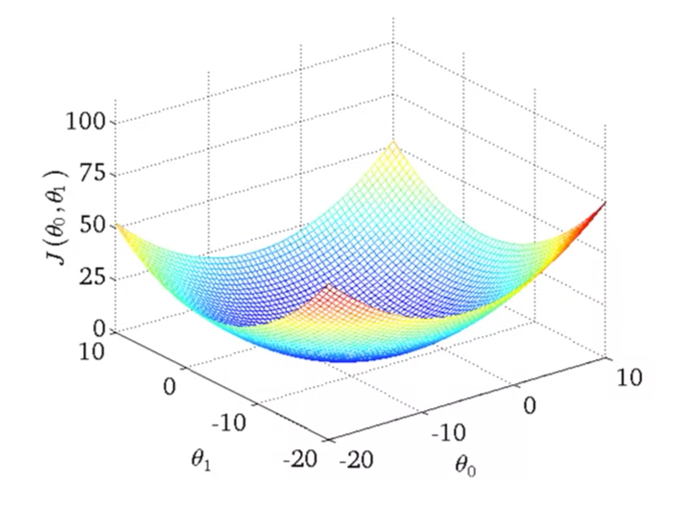
\includegraphics[scale=0.7]{img/J_bivariate.png} 
   \caption{Example of $J(\theta_0, \theta_1)$}
\end{figure}

In the common case of bivariate minimization problem one can use \textit{contour plot} which analyze the shape of the function at different heights. It is remarkable that points in the space $(\theta_0, \theta_1)$ which are on the same \textit{countour line} result in very different hypotesis. It is trivial to understand that,  in this case the minimum $J(\theta_0, \theta_1)$ is attained on the bottom of such a \textit{bowl-shaped} surface.

\begin{figure}[h]
    \centering
    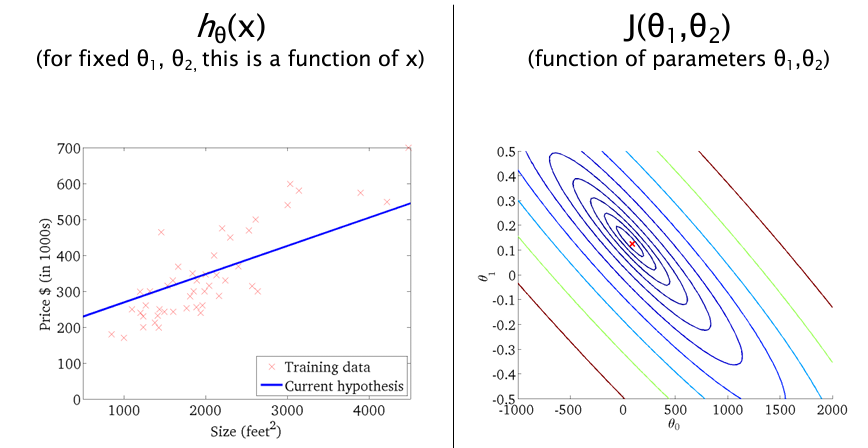
\includegraphics[scale=0.7]{img/contour.png}
\end{figure}

\section{Parameter learning: Gradient descent}
The objective here is to find a way to minimize a certain multivariate functional $J(\theta_1,..., \theta_n)$, the idea is using some methods that iteratively bring us to the minimum according to a certain criteria. In this paragraph we analyse the \textbf{Gradient Descent} algorithm, the main idea here is to start with some $\theta_0, \theta_1$\footnote{
    They are chosen either randomly or $\theta_i=0, \ \forall i$.
}, and keep changing them until $J$ evaluated at those parameters could reach (hopefully) the minimum, in the gradient descent this change is made up on the basis of the direction dictated by the \textbf{gradient of the functional} computed at the current parameters value (from which the name). The algorithm for GD is simply as follows:

\begin{figure}[h]
    \centering
    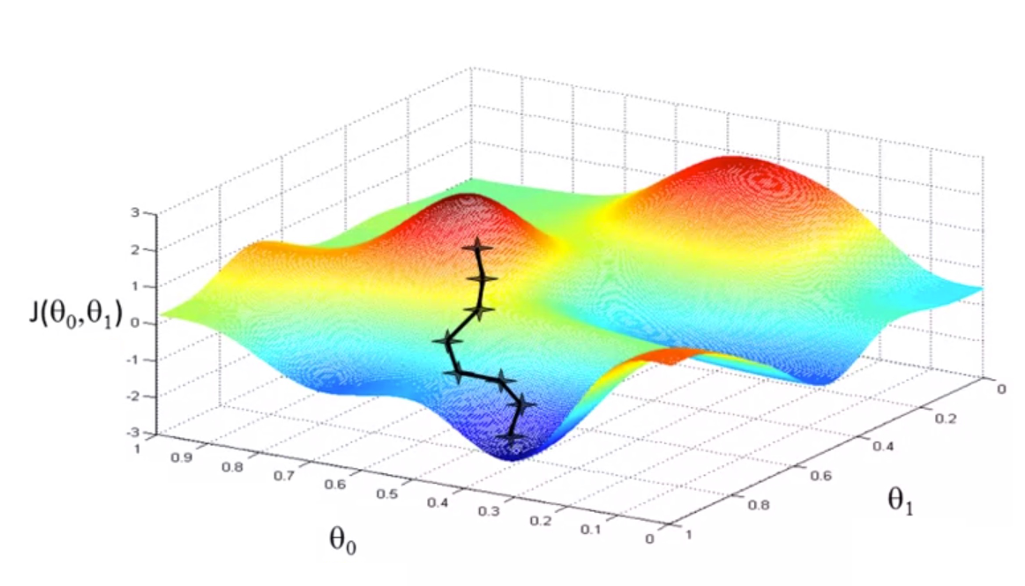
\includegraphics[scale=0.5]{img/nocvx_surf.png} 
\end{figure}

\begin{algorithm}[h]
    \caption{Gradient Descent}
    \begin{algorithmic}
        \While{!convergence}\\
           $\theta_j:=\theta_j-\alpha{\frac{\partial}{\partial{\theta_j}} J(\theta_0, \theta_1)}$
           \Comment{for $j$=0, $j$=1,...}
        \EndWhile
    \end{algorithmic}
\end{algorithm}

\noindent
The $:=$ symbol is associated with a \textit{simultaneous update}, note that if you put together for each $j$ the partial derivatives of $J$ you will obtain the gradient. The parameter $\alpha$ is called the \textbf{learning rate} and it must be properly chosen because:
\begin{itemize}
    \itemsep-0.2em
    \item If $\alpha$ is \textbf{too small}, then the convergence to the minimum (within a certain tolerance) could be very slow;
    \item If $\alpha$ is \textbf{too large} the algorithm can overshoot the minimum either failing to converge, or diverging.
\end{itemize}
Even when the learning rate is fixed the GD can converge to a (local) minimum since we are moving toward \textit{steep} directions which decrease the functional over time. If we apply the algorithm to the functional of the problem in (\ref{eq:ls1}) we obtain:
\begin{equation}
    \begin{aligned}
        &\theta_0=\theta_0-\alpha{\sum_{i=1}^{m}{(h_\theta(x^{(i)}-y^{(i)}))}}\\
        &\theta_1=\theta_1-\alpha{\sum_{i=1}^{m}{(h_\theta(x^{(i)}-y^{(i)}))} x^{(i)}}
    \end{aligned}
\end{equation}
this is known as \textbf{batch gradient descent} since for each step we use all the training samples. There are cases in which the minimization is particularly 'simple'. This happens when the functional is convex in $\theta$. Besides, for the class of convex functions a local minima is also a \textbf{global and only min}.

\section{Multivariate linear regression}
It is quite immediate to understand that the linear regression can be used also for a \textit{multivariate context} in which the samples are characterized by many features. In this context the hypotesis becomes:
\begin{equation}\label{eq:multivariate}
    h_\theta(x) = \theta_0{x_0}+\theta_1{x_1}+...+\theta_n{x_n}=\theta^T{x}
\end{equation}
In this case we have $n$ parameters and associated features $x_i$, so that the functional $J$ is function of $n$ parameters, in this case the partial derivatives to compute, obviously, will increase. Note that a \textit{fictitious} feature $x_0=1$ has been added with the purpose to employ a vector notation.\footnote{
    The great majority of tools and softwares which are used for machine learning exploit vector and matrices calculus to carry out their work.
}\\

\section{Data mean normalization}
Sometimes, before starting with the model construction, some preliminary operations are needed. For example, often it is better for the features being on a \textbf{similar scale}. In this  case we replace in each sample for each feature $x_i=x_i/s_i$ where $s_i$ can be either the range (max-min) for that feature or some index similar to variance/standard deviation.\\
Other times, one is supposed to normalize the data so that they can have a \textit{zero mean}. The trick here is replacing $x_i=x_i-\mu_i$, where $\mu_i$ is the mean for the $i$-th feature. Not rarely, you can find the two transformation combined such thet
\begin{equation}
    x_i=\frac{x_i-\mu_i}{s_i}
\end{equation}

\section{Debug of Gradient Descent algorithm}
The \textit{gradient algorithm} is clearly a descent method in the sense that -- being $k$ the $k$-th iteration -- it holds that $J(\theta_{k+1}) < J(\theta_{k})$, this is the same to state that the $J(\theta)$ function is required to be strictly decreasing. An \textbf{automatic convergence test} can be performed: for example the objective function $J$, had had a decreasing less than a certain threshold $\varepsilon=10^{-3}$ (for example).\\
Whether the algorithm is not working well the value for the \textbf{hyperparameter} $\alpha$ must be changed (for example decreasing it). One way to choose \textit{manually} $\alpha$ is by \textit{trial-error}\footnote{
    A more accurate method is the \textbf{backtracking line-search} which repeat some calculations until the so-called \textit{Armijo condition} is not met; however it requires that additive hypotesis are made on the regularity of the objective and its gradient.
}, choosing the $\alpha$ in a range and then plotting $J(\theta)$ as a function of the number of iterations. 

\begin{figure}[h]
    \centering
    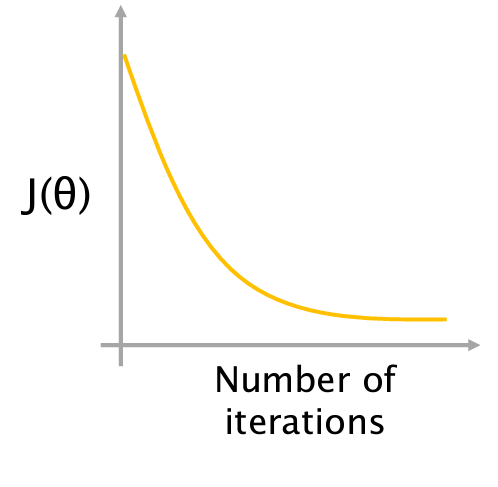
\includegraphics[scale=0.6]{img/alpha.png}
    \caption{Desired behaviour for $J(\theta)$ vs \# iterations}
\end{figure}
 
\section{Alternative to Gradient Descent}
There are alternative methods to gradient descent, for example the normal equation method which is derived by the analytical solution of the well-known \textbf{least-squares} problem. In this case $\theta$ is found by solving the system (normal equations):
\begin{equation}
    (X^T X)\theta = X^T{y}
\end{equation}
where the $X$ matrix contains the dataset features and $y$ is the vector with the "right answers". The solution of such a problem gives \textit{one-shot} the solution without proceeding by step as in the case  of gradient descent. The main limitation of such a method is the inversion of the matrix $X^T X$, which could be significantly slow if $n$ (number of features and parameters) is very large.\footnote{
    It is sufficient to think about the number of parameters involved in a problem of image classification. They are in a number of 3 billion for an RGB $1000\times1000$ image. 
}

\section{Polynomial regression}
\chapter{Logistic Regression}

The objective here is discussing the \textbf{Logistic regression} model which is used for \textbf{binary}, and also, \textbf{multiclass classification}. We will start from the hypotesis $h_\theta(x)$ used in the case of regression, we will analyze the aspects which will be maintained of it, and also the cons. 

\section{Classification vs Regression}
Coming back for a while to the problem of \textit{tumor classification}, suppose that a linear hypotesis can be used in order to separate the data. The comprehension of this concept is aided by the following figure: 
\begin{figure}[h]
    \centering
    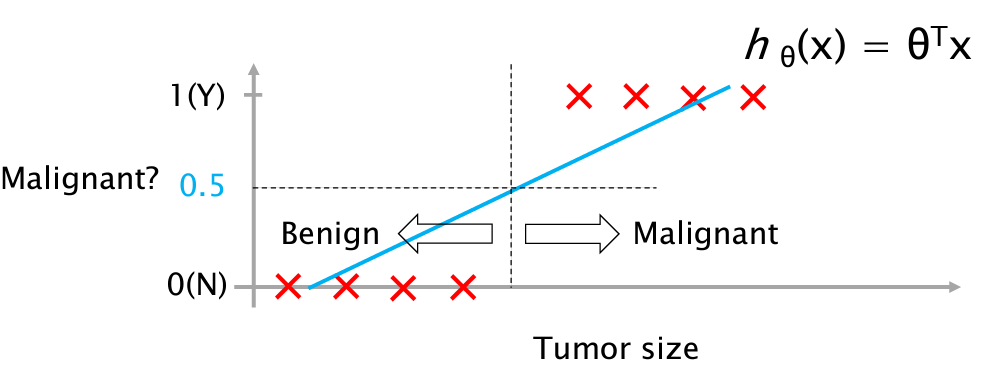
\includegraphics[scale=0.5]{img/Class_vs_Reg.png}
    \caption{Classification with linear hypotesis}
\end{figure}
The hypotesis $h_\theta(x)$ used in order to separate the two class is the line showed in blue. Since here we are not in the case of prediction of a continuous value, we have to find a way for shrink all possible output from the hypotesis in two values (Positive/Negative). At this point an idea could be using a threshold according which you can separate data from the two classes, that is:
\begin{equation} \label{eq:criteria}
    y=\begin{cases}
        1&\text{if} \ h_\theta(x)>0.5\\
        0&\text{if} \ h_\theta(x)\le{0.5}
    \end{cases}
\end{equation}
This appproach seems to work, until we do not change the data used for building the model. Let us consider, for example, the following scenario:
\begin{figure}[h]
    \centering
    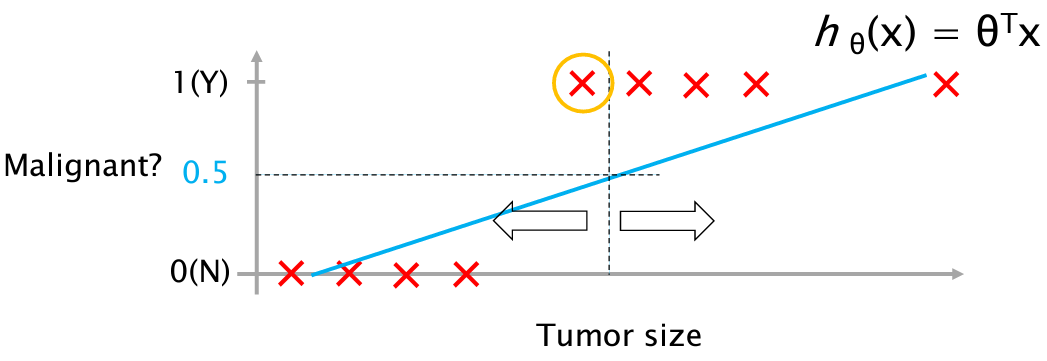
\includegraphics[scale=0.5]{img/Class_vs_Reg2.png}
    \caption{Effect of changing the dataset}
\end{figure}
It appears quite evident that one of the data for which we know that belongs to the positive class, is classified as negative.\\
This is not the only problem: we want that the predicted output\footnote{
    Later we will call it $\hat{y}$, for comparing it to the true output $y$.
}, that is the hypotesis is between 0 and 1, despite the fact of using a threshold this is not satisfied, since a linear function is \textit{unbounded}. At this point our reasoning leads to the formulation of the following two issues:
\begin{enumerate}
    \item A \textit{linear hypotesis} is not suitable for a classification problem, the performances would be awful also on the training set; 
    \item It is required that $$ 0 \le h_\theta(x) \le 1$$ this is not happening in the cases a linear hypotesis is employed.
\end{enumerate}
These are the main points that leads to the \textit{correct formulation} of \textbf{logistic regression}\footnote{
    The name \textit{logistic} is related to the fact that we are solving a dicotomic/binary classification problem.
}.

\section{Logistic regression}
The main concept behind \textit{logistic regression} is using a nonlinear function that saturates the hypotesis between 0 and 1. Basically we have to apply such a function which we will call $g(z)$ to the linear $\theta^T{x}$, such a function is called \textbf{sigmoid} or \textbf{logistic function}. It is depicted in the following and its expression is:
\begin{equation}
    g(z)=\frac{1}{1+e^{-z}}
\end{equation}

\begin{figure}[h]
    \centering
    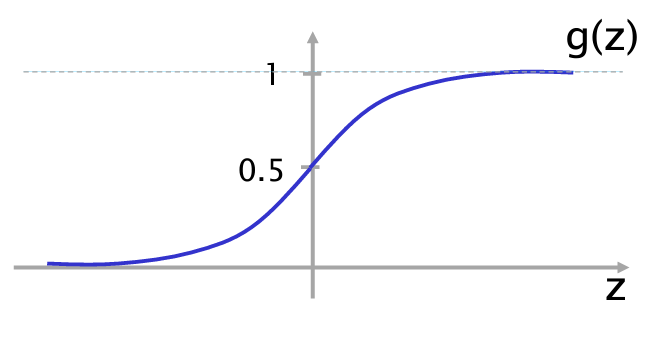
\includegraphics[scale=0.7]{img/logit.png}
    \caption{The logistic function $g(z)$}
\end{figure}

The output of such an hypotesis can be interpreted as \textit{the probability that the output y=1 on a given input x}, for example in the case of tumor classification a value of 0.7 of the hypotesis results in a prediction that for 70\% the given tumor (with its feature is malignant). In order to be mathematically formal we can say that 
\begin{equation}
    h_\theta(x)=P(y=1 | x; \ \theta )
\end{equation}
which is read "the probability for the output $y$ to be 1, given $x$, parametrized by $\theta$. Clearly, at the opposite we can compute
\begin{equation}
    P(y=0 | x; \ \theta) = 1 -P(y=1 | x; \ \theta )
\end{equation}
Here we can stick to the fact of having a threshold. More specifically, we use as an hypotesis $g(\theta^T{x})$ and we can use the criterion used in (\ref{eq:criteria}). Moreover for the particular function  $g(z)$ it is used we can say that, given the features $x$ then it is classified as positive if $\theta^T{x}\ge0$ or negative if $\theta^T{x}<0$, since the counterimage of 0.5 through $g(z)$ is equal to 0, as showed in the following figure.

\begin{figure}[h]
    \centering
    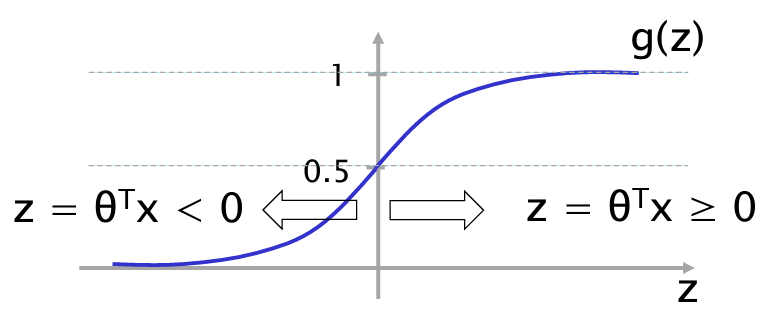
\includegraphics[scale=0.7]{img/logit2.png}
\end{figure}

It appears clear that the linear combination $\theta^T{x}$ is a (linear) \textbf{decision boundary} since it provides us with the information of having a positive or negative record. It is useful to give an example of this fact: 

\begin{figure}[h]
    \centering
    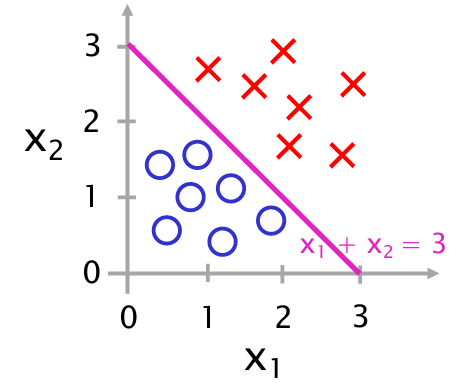
\includegraphics[scale=0.7]{img/decision_boundary1.png}
    \caption{Decision boundary}
\end{figure}

\noindent
Suppose we trained the model and the parameter theta resulted in being $\theta=[-3\  1 \ 1]^T$, this is the same to say that we assign \textit{positive class}to records with feature $x_1, x_2$ such that $\theta^T{x}$ is greater or equal than 0, negative class otherwise. Then, I can completely remove the record from the dataset and using such a decision boundary for doing classification. There are some cases in which due to the distribution of the data of each class, it is not possible to separate them with a linear decision boundary. In that case higher order nonlinear functions (eg. polynomials) must be used.

\section{Cost function for logistic regression}
We have seen in the former chapter about linear regression that a cost function is introduced to be minimized in order to find the parameter $\theta$ which are the best for our model.\\
In case we had a regression problem to be solved the functional $J(\theta)$ (Square Error) was a convex one, if we stick to the use of a sigmoidal function (and it is a proper choice for classification) the \textit{Square Error functional} becomes a non-convex one, so that the Gradient Descent Algorithm is not converging to a global minimum. What is changed for logistic regression is the \textbf{Loss function} associated to a single training sample. A particularly clever choice is the following:
\begin{equation}
    \text{Loss}(h_\theta(x),y) = \begin{cases}
        -\log(h_\theta)&\text{if} \ y=1\\
        -\log(1-h(\theta))&\text{if}\ y=0
    \end{cases}
\end{equation}

\begin{multicols}{2}

    \begin{center}
        \centering
        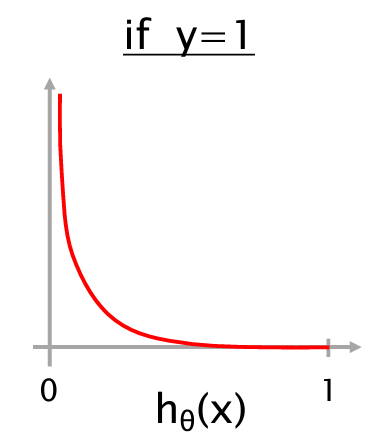
\includegraphics[scale=0.7]{img/Loss_y1.png}
    \end{center}
    \newcolumn
    \begin{center}
        \centering
        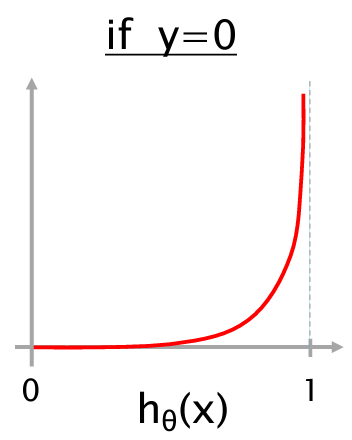
\includegraphics[scale=0.7]{img/Loss_y0.png}
    \end{center}
\end{multicols}

\noindent
Since the Loss function must penalize the objective to be effective in case the effective output is $y=1$ and the hypotesis (formulated with those parameters) would give 0, then the cost is very high. On the contrary a positive hypotesis with an actual output of $y=0$ will give to the functional a very high contribution, resulting in an high penalization (keep in mind that the functional must be minimized). This concept has a quite intuitive explanation as we have seen. \\
It would be useful having an \textit{overall functional} and with the aim of obtaining it, we badly exploit the fact that the output is logistic. In particular: 
\begin{equation}
    \text{Loss}(h(\theta),y)=-{\color{red}y} \log{h_\theta{(x)} - {\color{red}(1-y)}\log{(1-h_\theta(x))}}
\end{equation}

\noindent
The cost function coming from such a loss function is the following and it is denoted as \textbf{Binary cross-entropy cost function}:
\begin{equation} \label{eq:cross-entropy}
    J(\theta)=
    \underbrace{-\frac{1}{m}\sum_{i=1}^m \bigg[
        -{\color{black}y^{(i)}} \log{h_\theta{(x^{(i)})} - {\color{black}(1-y^{(i)})}\log{(1-h_\theta(x^{(i)}))}}
    \bigg]}_{\textsf{\color{orange}BINARY CROSS-ENTROPY COST FUNCTION}}
\end{equation}

\section{Training logistic regression}
Given the cost function (\ref{eq:cross-entropy}), we minimize it by using gradient descent algorithm, given an unknown $x$ the output is provided by using the hypotesis 
\begin{equation}
    h_\theta(x) = \frac{1}{1+e^{-\theta^\textsf{T}{x}}}
\end{equation}

\noindent
The algorithm of gradient descent follows the same step as in \textit{linear regression}, what is changed is the shape of the hypotesis $h_\theta(x)$.

\section{Multiclass classification}
Suppose we want to do a multiclass classification, for example for tagging mail as \textbf{SPAM, WORK, FRIENDS...} Can we use logistic regression in order to carry out such a task? The answer is YES, but with some modifications. In the sense that we can reformulate the problem in \textit{one class against the others}. The steps are the following: (A) We train a logistic regression classifier $h_\theta^{(i)}(x)$ in order to predict $P(y=i|x;\ \theta)$ for each class $i$. On a new input the prediction is done as follows:
\begin{equation}
    i=\arg\max_{i} h_\theta^{(i)}(x)
\end{equation}
where $i$ is the $i$-th class. Is this a good idea for a multiclass classification? Not so much! In the sense that the computational load grows of a factor $n$, with $n$ the number of classes. 

\section{Overfitting and Regularization}
In building a predictive model, there are usually two problems which we want to avoid: \textbf{underfitting and overfitting}. In the former case, provided that there are a small number of features, the learned hypotesis will not fit properly the training set. We can also say that there is an \textbf{high bias} in the data. In the latter case (overfitting) the learnt model has got excellent performances on the training set, in the limit case $J(\theta)=0$, but \textit{fails to generalize new examples}, in this case there are \textit{too many features}, so there is an \textit{high variance} in the data. \\
The configuration which is in the middle is the so-called \textit{just right}, and it is the one we want to reach aiming to have a good model. 

\begin{figure}[h]
    \centering
    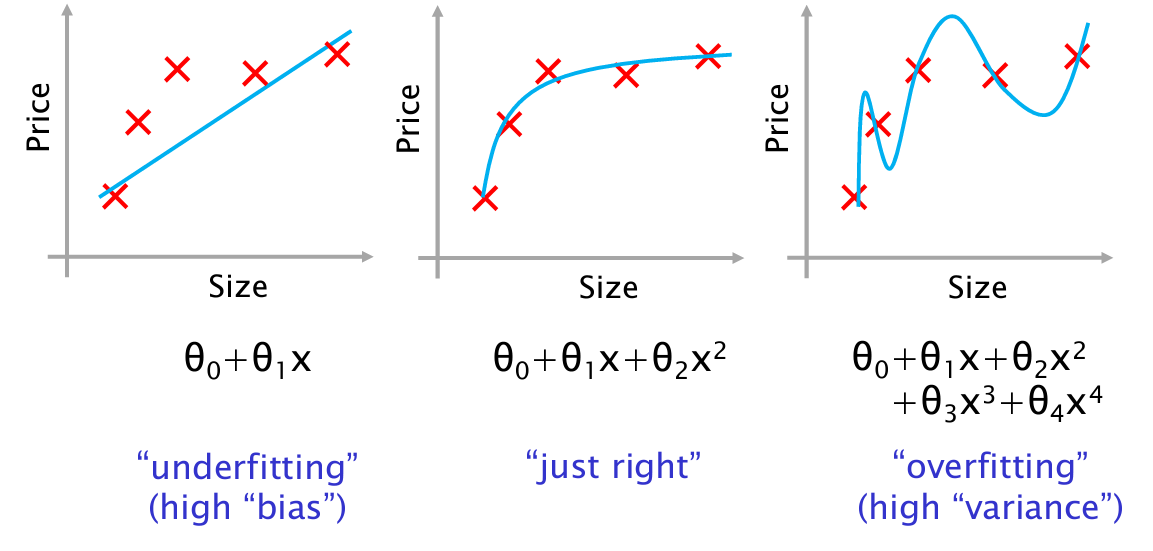
\includegraphics[scale=0.5]{img/over_under.png}
\end{figure}

\noindent
\textbf{What are the solutions for avoiding overfitting?} The first way is to reduce theb number of features the algorithm use for building the model (some techniques as PCA\footnote{
    PCA $\to$ Principal Component Analysis
} and LDA\footnote{
LDA$\to$ Linear Discriminant Analysis} can be used). Another way is introducing in the cost function a \textbf{regularization term}, its main purpose is to reduce the magnitude of the $\theta_i$ while keeping all the features. The regularization term acts directly on the parameters and it is proportional to the number of features. Using the regularization, simpler models can be obtained reducing the problem of overfitting the data. Let us consider for example the \textit{Square-error cost function}, when regularization is used it becomes:
\begin{equation} \label{eq:square_reg}
    J(\theta) = \frac{1}{2m} \sum_{i=1}^{m} (h_\theta(x^{(i)})-y^{(i)})^2 + \frac{\lambda}{2m} 
    \sum_{j=1}^{n} \theta_{j}^{2} 
\end{equation}
It is remarkable that the square-error cost function works on the $m$ training examples, while the regularization term\footnote{
    Do not confuse yourself with the \textit{normalization} which is done on the data
}interests directly the parameter of the model. The parameter $\lambda$ becomes another hyperparameter and we refer to it as the \textit{regularization parameter}. Clearly the optimization algorithm (Gradient Descent) must be updated accordingly. We also call the regularization in (\ref{eq:square_reg}) the $\ell_2$-regularization since it involves the $\ell_2$-norm definition. In the field of optimization models also the $\ell_1$-norm is considered, but in this case alternative techniques must be employed since the $\ell_1$-regularization makes the functional a non-differentiable one. Different algorithm, like ISTA and FISTA, have been developed in order to deal with such a type of optimization problem.
\chapter{Neural Networks: an introduction}
The idea of \textbf{neureal network (NN)} was introduced in the late 50s, in order to implement algorithm which could try to mimic the brain functionalities. They were very used in 80s, but their popularity decreased in the late 90s. Two determinant factors have aided the resurgence of such  technologies: the increasing in the quantity of data, and the increasing in computation capacity. For example, Neural Networks are used, among the others tasks, for performing classification.
We have understood that a linear hypotesis is not suitable for such a task, then nonlinearity is needed.\\
Now, let us imagine we want to build a model for classifying in a binary way, some images in two classes: CAR, NO CAR. An image is in general composed of pixels. Can we use \textit{logistic regression} for doing image classification? Let us consider a training set made up of $64\times{64}$ images, then 4096 pixels which is the same number for the parameter if we have a gray-scale image. If we have RGB images, the number of parameters grows by a $3$ factor, that is a number of parameters equal to $n=12288$, a huge number that makes highly unsuitable the logistic regression models. In this situation a neural network of some type is used.

\section{Ideas underlying neural networks}
Before going on through the discussion of (Artificial) Neural Networks, we have to just mention how a biological neuron is made.

\begin{figure}[h]
    \centering
    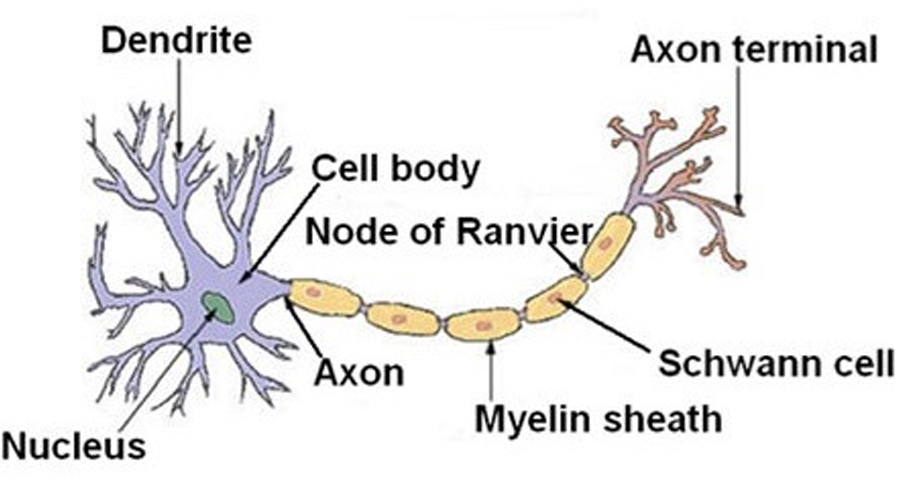
\includegraphics[scale=0.5]{img/bio_neuron.png}
\end{figure}
\noindent
Three are the main components of a neuron:
\begin{enumerate}
    \itemsep-0.2em
    \item Some inputs wires (\textbf{Dendrites})
    \item A \textbf{Nucleus} which is the \textit{computational unit}
    \item An output wire (\textbf{Axon})
\end{enumerate}
Clearly such a type of cells are connected each other by mean of \textit{synapses} realized by neutrotransmitters. \\
The \textbf{artificial neural newtork} has exactly the same structure of a biological one whose building blocks are some \textit{artificial neurons} made up of the same three basic elements, since it has got: (i) some inputs which are the features, (ii) a computation unit that performs a weighted sum of the features, (iii) an output which is the result of an \textbf{activation function} which often can be a sigmoid. [From this point we can see the strong relationship with the logistic regression.] Other activation functions can be used, besides another example is the \textbf{ReLU}.

\begin{figure}[h]
    \centering
    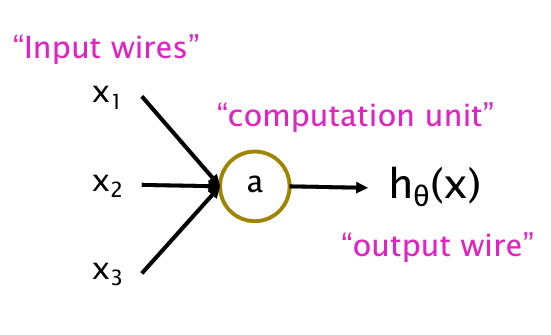
\includegraphics[scale=0.7]{img/artificialneuron.png}
    \caption{Structure of an artificial neuron}
\end{figure}

\subsection{Notation} 
In the following some notation is introduced that will be used in the remaining part of the course dealing with neural networks. When we put together some artificial neurons, what we obtained in general is a \textbf{multilayer perceptron} or \textit{classical NN}. The \textit{layer 0} is the input layer, the following are numbered as first, second layer and so on. In each layer we can find one or more computational units. For example the first layer of the showed NN has 3 computational units (without considering the unit 0 which is associated to the bias). The notation $a_i^{[j]}$ indicates the \textbf{activation} in the \textbf{i-th unit} in the \textbf{$j$-th level} of the network, while $\Theta^{[j]}$ is the weighting matrix for the  $j$-th layer of the network.\footnote{
    The intermediate layers of a neural network are called \textbf{hidden layers} since the output produced is hidden and are generated by linear and non linear combination of the features.
}
Usually also the input are renamed as \textit {zero-layer activation}, then are indicated with $a_i^{[0]}$. For the presented MLP\footnote{
    multilayer perceptron
} let us try to write all of the activation of each layer:
\begin{align*}
    &a_1^{[1]} = g(\Theta_{10}^{[1]} a_0^{[0]} + \Theta_{11}^{[1]} a_1^{[0]}+\Theta_{12}^{[1]}a_2^{[0]}+\Theta_{13}^{[1]}a_3^{[0]})=g(z_1^{[1]})\\
    &a_2^{[1]} = g(\Theta_{20}^{[1]} a_0^{[0]} + \Theta_{21}^{[1]} a_1^{[0]}+\Theta_{22}^{[1]}a_2^{[1]}+\Theta_{23}^{[1]}a_3^{[0]})=g(z_2^{[1]})\\
    &a_3^{[1]} = g(\Theta_{30}^{[1]} a_0^{[0]} + \Theta_{31}^{[1]} a_1^{[0]}+\Theta_{32}^{[1]}a_2^{[0]}+\Theta_{33}^{[1]}a_3^{[0]})=g(z_3^{[1]})\\
    &a_1^{[2]} = g(
        \Theta_{10}^{[2]}a_0^{[1]}+
        \Theta_{11}^{[2]}a_1^{[1]}+
        \Theta_{12}^{[2]}a_2^{[1]}+
        \Theta_{13}^{[2]}a_3^{[1]} 
    )=g(z_1^{[2]})
\end{align*}
\noindent
In this case the weighting matrices are for the first layer $\Theta^{[1]}\in\mathbb{R}^{3,4}$, for the second layer is $\Theta^{[2]}\in\mathbb{R}^{1,4}$.

\subsection{Different types of NN for different types of purposes}
A neural network can be used either for binary or multiclass classification. In the former case the last layer has got one neuron whose activation is 0 or 1, in the latter case we have a neuron for each class in a level that is (how we will see) the \textit{softmax layer}. Moreover a neural network is said to be \textbf{shallow} (typically) when it is made up of a number of layers which is less than seven, otherwise we have a \textbf{deep neural network}.

\begin{figure}[h]
    \centering
    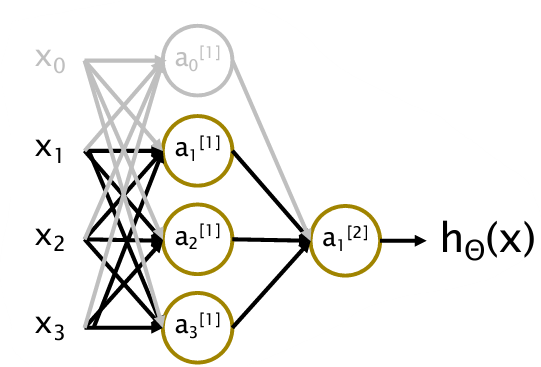
\includegraphics[scale=0.6]{img/neuron_spec.png}
\end{figure}

\section{Logistic regression as a NN}
If we better analyse the structure of a neuron and the path going from the input to the output of it, we will discover that it is something very similar to what we have seen in the case of logistic regression, where we have combined a linear part with a non linear one in order to correctly perform the (binary) classification task.\\
Now, let us suppose we want to perform a binary classification a set of images, in particular we want distinguish when they are cars or not. Can we use logistic regression in order to perform such a task? NO! It could be very slow and inefficient: a logistic regression (that is a single neuron) cannot perform in a good way such a task, then a neural network is used in this case. The next step is: how can we represent an image as a vector of features? We know that a gray-scale image can be represented as a matrix of numbers in the range [0-255], if the image is RGB we have a different matrix for each one of the channel R, G and B. We can turn the matrix into a vector by simply unrolling it row by row, in a way that each single pixel of each one of the channel is a feature for our classification problem. This example was just to present the problem of \textbf{vectorization}, that in the field of neural network is a very common operation which is done on the data in order to make them suitable for network itself.\\

\noindent
We have seen in the logistic regression that our \textbf{predicted value} $\hat{y}$ (which was the hypotesis), is nothing but the result of a sigmoidal function applied to the linear combination $w^T{x}+b$, where $w$ are the weights, $b$ is the bias while $x$ is the feature vector. Then we have that: 
\begin{equation}
    \hat{y}=a=\sigma(w^T{x}+b)
\end{equation}
How we mentioned, this is exactly the work performed by a neuron from the inputs to the output. Furthermore, we have seen that for the logistic regression a different cost function must be considered in order not to dealing with \textit{non-convex optimization problem}. For the description of the logistic regression as a single-neuron NN, nothing change a part from few differences in the notation. In fact we indicate the hypotesis $h_\theta(x)$, with the \textit{predicted value} $\hat{y}$, while the $\theta_i$ parameters are split in weights $w$ and a single bias $b$. Another difference we can find in the field of NN, is that the partial derivatives of the functional $J$ to be minimized with respect to the weights/bias, that is 
\begin{equation}
    \frac{\partial{J}}{\partial{w}}, \quad 
    \frac{\partial{J}}{\partial{b}}
\end{equation}
are denoted simply with $dw$ and $db$, in order to make lighter the notation. The \textit{gradient descent step} in order to decrease the functional becomes:
\begin{align*}
    &w = w - \alpha\ {dw}\\
    &b = b - \alpha\ {db}
\end{align*}
Now, \textbf{How can we compute the partial derivatives?} For sure, we can say that no explicit analytic calculation are performed, instead a very powerful tool that is the \textbf{automatic differentiation} leveraging on the so-called \textbf{computation graph} is used. The main concept behind it is to express a function by using \textit{intermediate auxiliary variables} and computing the derivatives by using the \textbf{Leibnitz's Chain Rule}.

\section{Automatic differentiation and computation graph}
Suppose we have a function
\begin{equation}\label{eq:exJ}
    J(a,b,c)=3(a+bc)
\end{equation}
we want to compute the ppartial derivatives of $J$ with respect to the three variables $a,b,c$. We can introduce some intermediate variables which can be called
\begin{equation*}
    u=bc \quad  v=a+u
\end{equation*}
Our function $J$ becomes: $J=3v$. In this way we have split the original function in trhee different simpler functions. This procedure can be graphically represented as shown in the figure:

\begin{figure}[h]
    \centering
    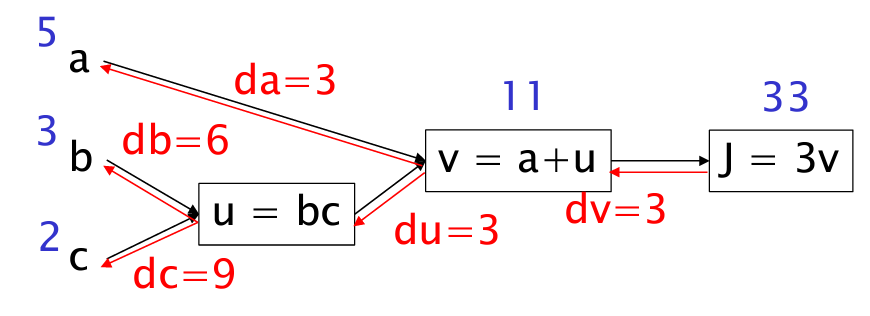
\includegraphics[scale=0.5]{img/computation_graph.png}
    \caption{Computation graph for $J=3(a+bc)$}
\end{figure}
\noindent
In particular from the input $a,b,c$, we can compute the value of the intermediate variable $u$, which can be used for obtaining $v$, finally we can compute $J$. This path from $(a,b,c)\to{J}$ is called \textbf{Forward Propagation}. Now, what about the partial derivatives? We can proceed step by step, doing an inverse path from $J\to(a,b,c)$, intuitively such a path is the \textbf{Backward propagation}, here the \textit{Chain rule} is used in order to carry out 'gradually' the computation of the partial derivatives.
The following steps are done:
\begin{align*}
    &\frac{\partial{J}}{\partial{v}}\doteq{\color{red}\mathbf{dv}}=\mathbf{\color{red}3} \quad
    \frac{\partial{J}}{\partial{u}}\doteq{\color{red}\mathbf{du}}=
    \frac{\partial{J}}{\partial{v}} \frac{\partial{v}}{\partial{u}} = 3 \cdot 1 = \mathbf{\color{red}3}\\
    &\frac{\partial{J}}{\partial{a}} \doteq{\color{red}\mathbf{da}}=
    \frac{\partial{J}}{\partial{v}} \frac{\partial{v}}{\partial{a}} = \mathbf{\color{red}3} \quad
    \frac{\partial{J}}{\partial{b}}\doteq{\color{red}\mathbf{db}}=
    \frac{\partial{J}}{\partial{v}}\frac{\partial{v}}{\partial{u}}\frac{\partial{u}}{\partial{b}}=3\cdot{1}\cdot{c}=3c=\mathbf{\color{red}6}\\
    &\frac{\partial{J}}{\partial{c}}\doteq{\color{red}\mathbf{dc}}=
    \frac{\partial{J}}{\partial{v}}\frac{\partial{v}}{\partial{u}}\frac{\partial{u}}{\partial{c}}=3\cdot{b}=\mathbf{\color{red}9}
\end{align*}
The procedure we have just shown is THE way in which are computed the derivatives in the field of Neural Network. Clearly, the same reasoning we have done for the functional (\ref{eq:exJ}) can be repeated for the \textit{loss function} used for the case of logistic regression. The figure below shows the final result of forward and backward propagation applied for the \textbf{cross-entropy loss function}.
\begin{figure}[h]
    \centering
    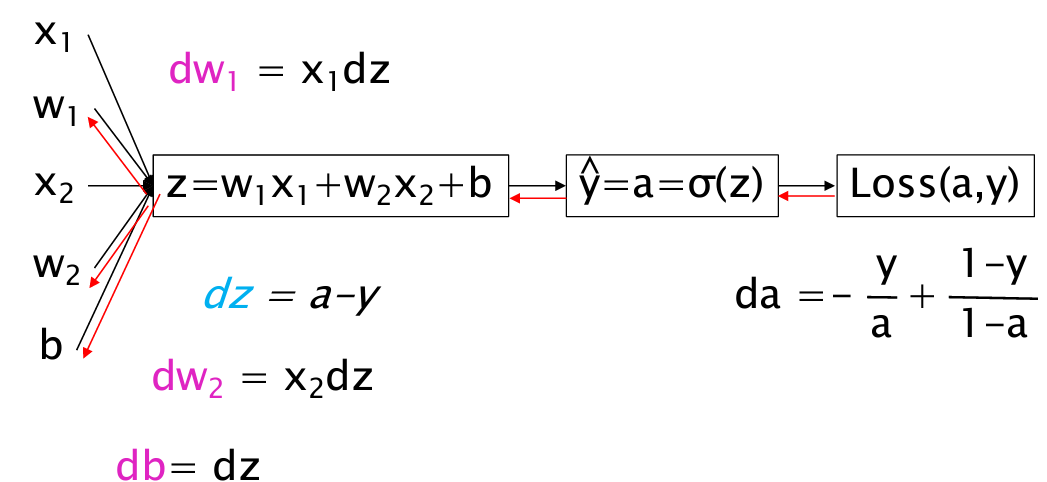
\includegraphics[scale=0.5]{img/compgraph_Loss.png}   
\end{figure}

\subsection{Feedback and Backward propagation for Logistic Regression}
For a single training sample we have that the feedback and backward propagation mathematical steps are the following:
\begin{multicols}{2}
    \noindent
    \textbf{FORWARD PROPAGATION}
    \begin{align*}
        &z_i=w^T{x^{(i)}}+b \quad \text{(linear part)}\\
        &\hat{y}_i=a_i=\sigma(z_{i})   \quad \text{(activation)}\\
        &J_{i}=-[y_{i}\log{a_{i}}+(1-y_{i})\log(1-a_{i})] \\
        & \quad \quad \text{(cost function)}
    \end{align*}
    \newcolumn\\
    \noindent
    \textbf{BACKWARD PROPAGATION}
    %\begin{align*}
        %&z=w^T{X}+b \quad \text{(linear part)}\\
        %&\hat{y}=a=\sigma(z)   \quad \text{(activation)}\\
        %&J=-\frac{1}{m}[y\log{a}+(1-y)\log(1-a)] \\
        %& \quad \quad \text{(cost function)}
    %\end{align*}
    \begin{align*}
        &dz_i = a_i-y_i\\
        &dw_i={x^{(i)}}{dz_i}\\
        &db_i=dz_i
    \end{align*}
\end{multicols}
\noindent
Whether we extend such computations to the whole dataset, we have matrices and vectors instead of vectors and scalars. In particular:
\begin{multicols}{2}
    \noindent
    \textbf{FORWARD PROPAGATION}
    \begin{align*}
        &z=w^T{X}+b \quad \text{(linear part)}\\
        &\hat{y}=a=\sigma(z)   \quad \text{(activation)}\\
        &J_{i}=-1/m \sum [y\log{a}+(1-y)\log(1-a)] \\
        & \quad \quad \text{(cost function)}
    \end{align*}
    \newcolumn\\
    \noindent
    \textbf{BACKWARD PROPAGATION}
    %\begin{align*}
        %&z=w^T{X}+b \quad \text{(linear part)}\\
        %&\hat{y}=a=\sigma(z)   \quad \text{(activation)}\\
        %&J=-\frac{1}{m}[y\log{a}+(1-y)\log(1-a)] \\
        %& \quad \quad \text{(cost function)}
    %\end{align*}
    \begin{align*}
        &dz = a-y\\
        &dw= \frac{1}{m} (X^T{dz^T})\mathbf{1}\\
        &db=\frac{1}{m}(\mathbf{1}^T{dz})
    \end{align*}
\end{multicols}
\noindent
Where $\mathbf{1}$ is a column vector with all ones. After having performed the forward and backward steps, both weights and bias must be updated as follows: 
\begin{equation}
    w:=w-\alpha\cdot{dw} \quad b:= b-\alpha\cdot{db}
\end{equation}
Such steps must be repeated until convergence (in some sense). Keep always in mind that $dw$ and $db$ are the partial derivatives of the cost function with respect to the weights and bias.

\section{Training Neural Networks}
Till now we have seen the optimization procedure of the \textit{logistic regression} as a single neuron. However, we know that a neural network is made up of several layers which in turn are composed of several neurons (computational units). The objective here is to understand how we can generalize the \textbf{optimization procedure} in the case when the whole neural network must be trained (in particular the parameters for each neuron, for each layer must be computed).

\begin{figure}[h]
    \centering
    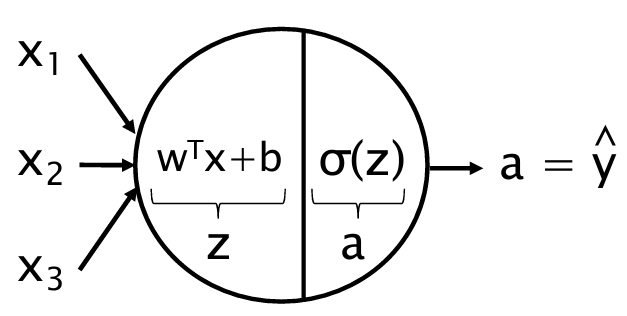
\includegraphics[scale=0.4]{img/single_log_neuron.png}
    \caption{Single neuron in form of logistic regression}
\end{figure}
\noindent
We are going to proceed step by step starting from a single neuron, going to the whole layer analyzing both the forward and backward propagations aimed to generalize the gradient descent algorithm to the whole network. For sake of simplicity but without loss of generality, the analysis has been conducted on a 2-layer NN. In the following the activation function will be indicated with $g$  in order to generalize to the use of different functions which can be used.

\subsection{Forward propagation}

\subsubsection{Single neuron, single sample}
\begin{multicols}{2}
    \begin{center}
        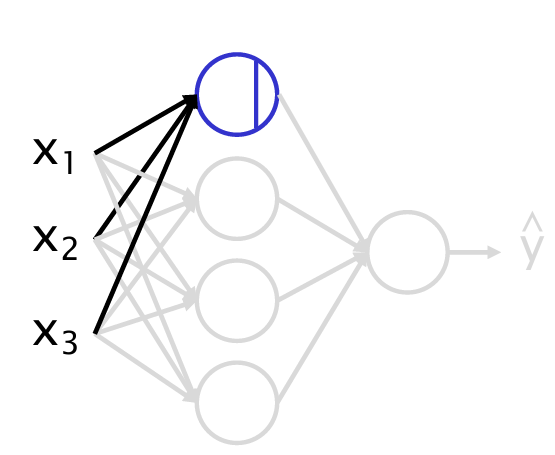
\includegraphics[scale=0.5]{img/2L_single.png}
    \end{center}
    \newcolumn
    A single neuron of the layer is considered, which clearly has his own weights and bias.
    \begin{equation} \label{eq:single_neuron}
        \begin{aligned}
            &z_1^{[1]}=w_1^{[1]T}{x}+b_1^{[1]}\\
            &a_1^{[1]}=g(z_1^{[1]})
        \end{aligned}
    \end{equation}
    The function $g$ can be something different with respect to a sigmoid. Only one sample $x$ of the dataset is considered.
\end{multicols}

\subsubsection{Single Layer, single sample}
\begin{multicols}{2}
    \begin{center}
        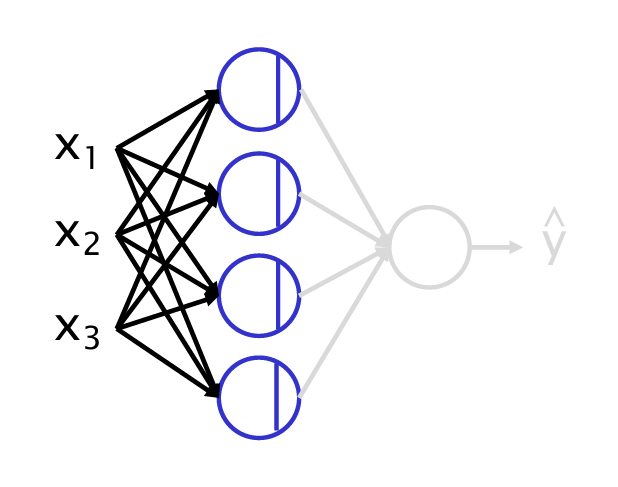
\includegraphics[scale=0.45]{img/2L_layer.png}
        \vspace{-0.5cm}
    \end{center}
    Considering all the neurons in the first layer, we have the (\ref{eq:single_neuron}) repeated four times, that is: 
    \begin{equation*}
        \begin{aligned}
            &z_i^{[1]}=w_i^{[1]T}{a^{[0]}}+b_i^{[1]}\\
            &a_i^{[1]}=g(z_i^{[1]})
        \end{aligned}, \quad i=1,...,4
    \end{equation*}
    Here the only difference is that we have indicated in terms of activations the input. In a more compact form we can say that:
    \begin{equation}
        \begin{aligned}
            &z^{[l]}=W^{[l]}a^{[l-1]}+b^{[l]}\\
            &a^{[l]}=g(z^{[l]})
        \end{aligned}
    \end{equation}
    where $l$ indicates the $l$-th layer of the network.
 \end{multicols}

\subsubsection{Single layer, whole dataset}
Till now we have seen the \textit{forward step} for a single neuron and for a layer of the network. What if considering the whole dataset instead of a single sample? The vector $z$ of the linear combination becomes a matrix in which the \textbf{$i$-th row} contains the linear combination for the \textbf{$j$-th} sample of the activation of the past layer. We have:
\begin{equation}
    \begin{aligned}
        &Z^{[l]}=W^{[l]}A^{[l-1]}+b^{[l]}\\
        &A^{[l]}=g^{[l]}(Z^{[l]})
    \end{aligned}
\end{equation}
Here is noticeable that the activation function can be different for each level of the network. This is the reason why we put the $l$ superposed also on the $g$.
\subsection{Backward propagation}
For the case of backward propagation we give directly the result in the most general case in which the loss function is even different than the \textit{cross-entropy}. Then, we have:
\begin{equation}
    \begin{aligned}
        &dZ^{[l]}=dA^{[l]}.*g^{[l]'} \ Z^{[l]}\\
        &dW^{[l]}=\frac{1}{m} (dZ^{[l]}A^{[l-1]T})\\
        &db^{[l]}=\frac{1}{m} \text{sum}({dZ^{[l]}})=\frac{1}{m}dZ^{[l]}\mathbf{1}\\
        &dA^{[l-1]}=W^{[l]T} dZ^{[l]}
    \end{aligned}
\end{equation}
For the output layer $dA^{[L]}=A^{[L]}$. The gradient step must be performed for each layer once all the derivatives have been computed: 
{\large{
    \begin{equation}
        W^{[l]}:= W^{[l]}-\alpha\cdot{dW^{[l]}} \quad    b^{[l]}:=b^{[l]}-\alpha\cdot{db^{[l-1]}}
    \end{equation} 
}}
The whole procedure of forward and backward propagation can be schematically represented by using a block diagram: 

\begin{figure}[h]
    \centering
    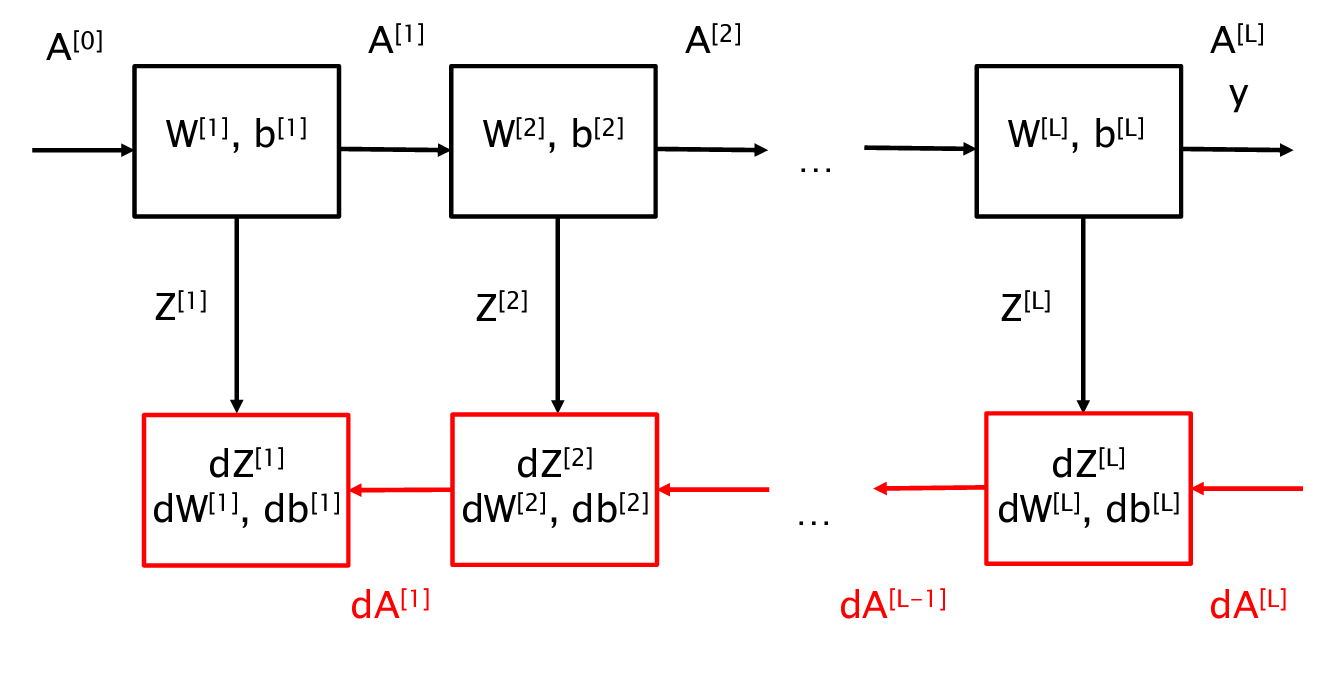
\includegraphics[scale=0.5]{img/block_diagram_GD.png}
    \caption{Block diagram for the GD}
\end{figure}

\section{Activation functions}
At different layers of a neural network, different activation functions can be used. Till now we have seen the sigmoid, since it is the one arising in the case of \textit{logistic regression}. Other choices can be done according to the needed convergence property and the task to be performed. The most common used activation functions are reported in the figure below (in the description there is also the definition).

\begin{figure}[h]
    \centering
    \subfigure[$\sigma(z)={1}/{(1+e^{-z}})$]{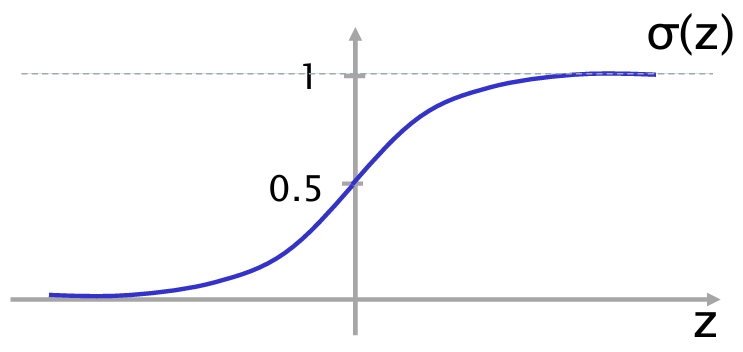
\includegraphics[scale=0.45]{img/sigmoid.png}}
    \subfigure[$\tanh(z)=(e^z-e^{-z})/(e^{z}+e^{-z})$]{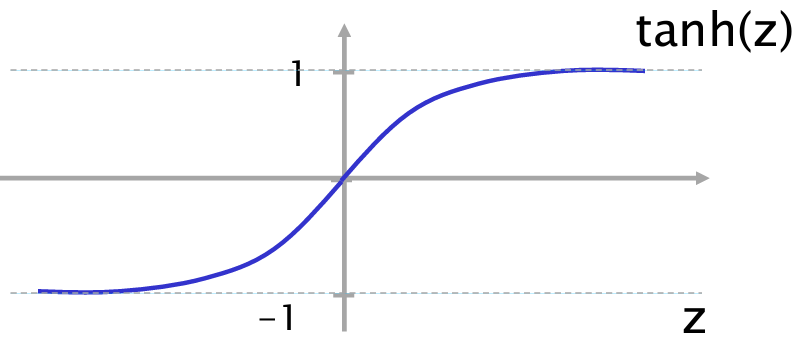
\includegraphics[scale=0.45]{img/tanh.png}}
    \subfigure[$\text{ReLU}(z)=\max(0,z)$]{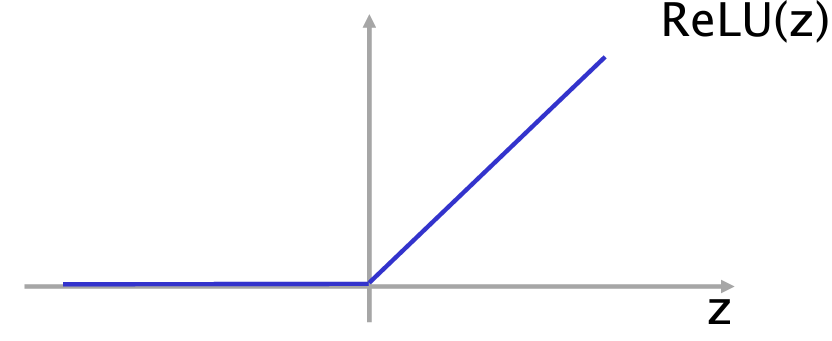
\includegraphics[scale=0.45]{img/ReLU.png}}
    \subfigure[$LeakyReLU(z)=max(\varphi{z}, z)$]{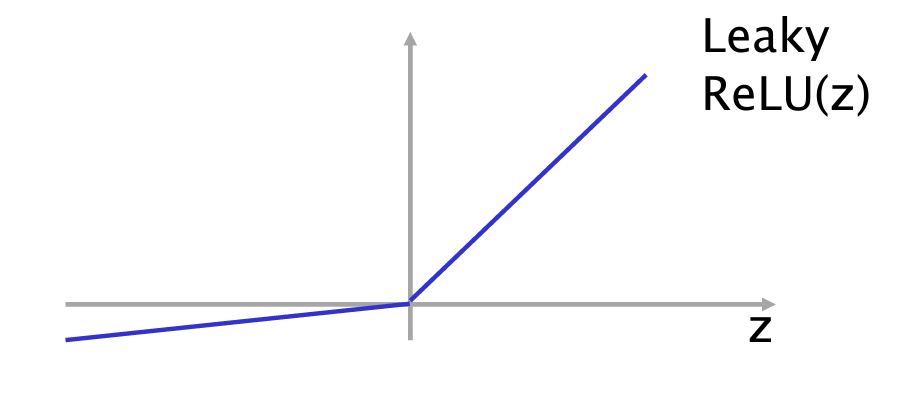
\includegraphics[scale=0.45]{img/LeakyReLU.png}}
    \caption{Some activation functions}
\end{figure}
\noindent
Note that in the $LeakyReLU(z)$ there is a parameter $\varphi$, this is in order to deal with the fact that the derivatives of $ReLU(z)$ for $z<0$ is equal to zero. Such an $\varepsilon$ becomes an hyperparameter.

\section{Initialization of the parameters}
When we have seen the \textit{linear regression} and the \textit{logistic regression}, we have said that the parameters $\theta_i$ would have been initialized for example to zero. This does not work in the case of neural networks. It has been demonstrate that the \textbf{zero-Initialization} of the weights leads to a problem of \textbf{Symmetric weights}, that is after each update, parameters associated to the inputs going to the next hidden layer unit are \textit{identical}. One possible solution, at least for simple NN, is to iniatialize randomly the weights $W^{[l]}$ and biases $b^{[l]}$ with numbers in the interval $[-\epsilon, \epsilon]$. Indeed, more sophisticated approaches are needed in the case of deep neural networks.

\section{Training a neural network (Recipe)}
Once we have presented the main issues related to neural networks and their training, we are ready to give a list of steps aimed to the training: 
\begin{enumerate}
    \itemsep-0.3em
    \item[0.] Pick a network structure, fix the numer of input and output unit with respect to number of inputs and number of classes respectively; the \textit{number of hidden layers} can be decided at this stage and also the number of neurons for each one of such layers. This are all \textbf{hyperparameters}.
    \item Randomly initialize the weights
    \item Implement \textit{forward propagation} in order to get the estimate $\hat{y}^{(i)}$ for any $x^{(i)}$;
    \item Implement code to compute the cost function $J(w,b)$ (this is another choice that we have done according to the task to be performed); 
    \item Implement \textbf{backward propagation} to compute partial derivatives (of the functional wrt the parameters);
    \item Use \textbf{gradient descent} or other optimization methods together with backward propagation to try to minimize $J(w,b)$.
\end{enumerate}

\section{Hyperparameters}
In the field of neural networks is fundamental the distinction between \textbf{parameters} and \textbf{hyperparameters}. The former ones are the ouput of the training phase, they are those that characterize a model from another. The latter ones are related to the choices that the \textit{machine learning engineer} makes in order to improve the performances of the predictive model. Examples of hyperparameters are:
\begin{itemize}
    \itemsep-0.3em
    \item Learning rate $\alpha$ of the gradient descent; 
    \item Number of iterations of the optimization algorithm; 
    \item Number of hidden layers and for each one the number of computational units; 
    \item Activation functions for each layer and related hyperparameters (eg. in the Leaky ReLU there is $\varphi$ to choose)
 \end{itemize}
 The \textbf{optimal (in some sense) configuration} must be found. 

\section{Training, Development, Test sets}
When we want to build a machine learning model, we must have a \textbf{dataset}. Clearly, since the optimal configuration of the network has to be found, only a portion of this data is used for the training phase. In general the dataset is divided into three portions:
\begin{figure}[h]
    \centering
    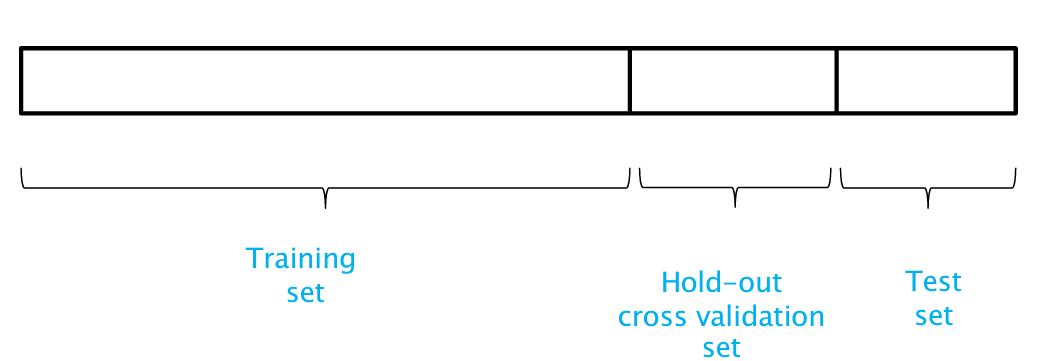
\includegraphics[scale=0.5]{img/dataset.png}
    \caption{Traditional dataset partitioning}
\end{figure}

In the past, when not too much data was available the ratios were 60\%, 20\%, 20\%; however with the increasing of the data availability the trend is using as much data as possible for the training set (98\%) and the remaining part for development and test (1\% for each one).
 \begin{description}
    \item[Training set] Is the biggest part of the dataset which is used for building the model (obtaining parameters). On this set could be necessary preliminary operations of \textit{data preparation} (eg. normalization, data augmentation and so on).
    \item[Cross-Validation/Development set] Is the set used for evaluating different models (not necessarily different architectures, but also different hyperparameters). The data distribution should match with the one in the training set. The validation set which is used, clearly is the same for all the selected models.
    \item[Test set] Once the model has been chosen a test on data that the network has never seen should be done. Such data can be extracted from the dataset, or coming from other sources making optional the presence of this type of set.
\end{description}

Once having defined how it is split the dataset, the \textbf{model selection} takes place, performing the following procedure. Given different models:
\begin{itemize}
    \item I minimize the cost function on the training set finding the parameters for each of them; 
    \item Compute the cross-validation error (on the validation set) using the output parameters for that model; 
    \item Chosse the model with the lowest error, then evaluate the \textbf{generalization performances} (using the \textit{test set}).
\end{itemize}
\chapter{Evaluating learning algorithm}

\section{Underfitting and overfitting data}
Once the model has been built, we are interested in detecting wheter out model is affected by either \textit{high bias} or \textit{high variance}. In order to better formalize such a concept is interesting to analyze the graph below: 

\begin{figure}[h]
    \centering
    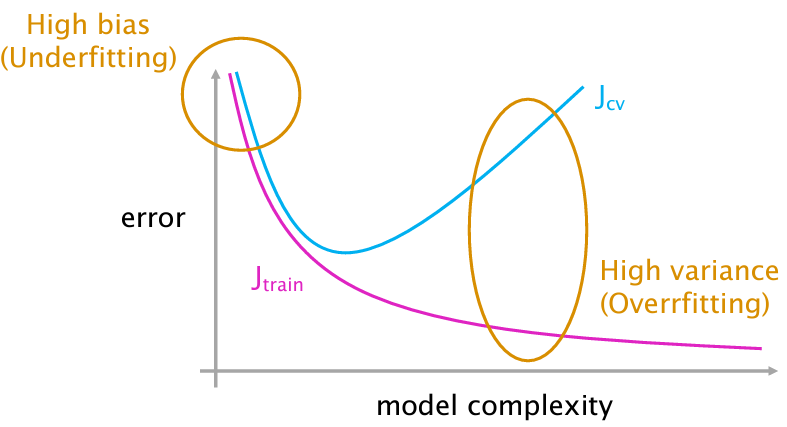
\includegraphics[scale=0.6]{img/bias_variance.png}
    \caption{High-bias vs High-variance}
\end{figure}

\noindent
Only for diagnostic purposes, we collect the data related to the error that the model does on the training data. Clearly the cost function $J_{\text{train}}$ is very high with a  very simple model because the network has not seen a sufficient amount of data. The error on the training set becomes smaller and smaller with the increasing complexity (number of features and so number of parameters of the model). What is very interesting to observe is what happen to the cost function when the validation data are used and the model complexity is growing. At start with a very simple model we have similar cost function, in fact $J_{\text{cv}}$ is very similar to $J_\text{train}$. This situation arises when the model is too simple and the model is \textbf{underfitting the data}. At the opposite when the model complexity grows there is a big difference between the two cost functions. This is related to the fact that the model has very bad performances with never seen data. In this situation we are in front of a problem of \textbf{overfitting the data}: the model has learnt by heart the data, but it is not able to generalize. \\
Both situations must be avoided, as they make a model unusable! The same reasoning can be done by a \textit{different perspective}, that is analyzing what happen to the $J_*$ in function of the dataset size. I have an \textit{high-bias} if at the end of the training phase I have a big error (\textit{with respect  to the human error}). On the other hand, I have an \textit{high-variance} if the model has bad performances on new data, or differently said, the two errors are very different. Note that, both high-variance and bias can be present in some situation. In particular in all cases when the error on training data is high and this is at the same time distant from the cross-validation error.

\begin{figure}[h]
    \centering 
    \subfigure[High-bias]{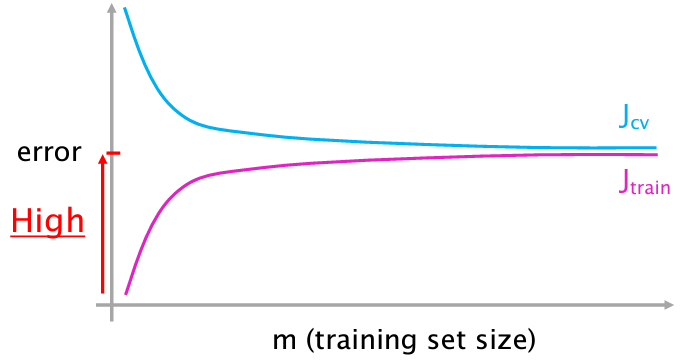
\includegraphics[scale=0.5]{img/bias_variance2.png}}
    \subfigure[High-variance]{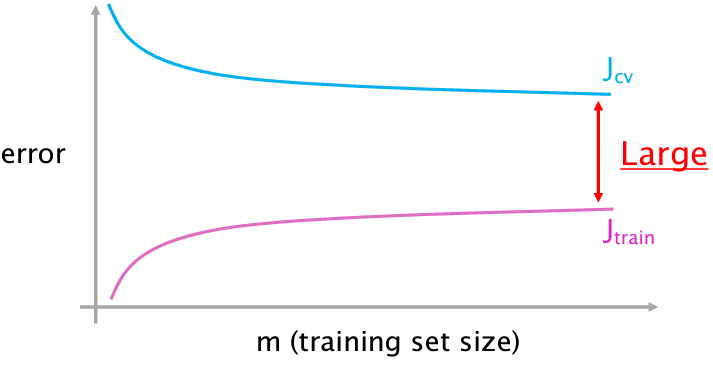
\includegraphics[scale=0.5]{img/bias_variance3.png}} 
\end{figure}

\section{Metrics for model evaluation}
\subsubsection{Motivation}
Given a model which makes a \textit{cancer classification}, suppose we want to evaluate its performance by using the so-called \textbf{accuracy}, we get a 1\% error on the validation/test set. From the labeled data, furthermore, can be analyzed for example that among all the patients only the 0.5\% has cancer. In this case if we take a \textit{Naive classifier} that ignoring the output predicts always $y=0$ (no cancer), such a classifier has better performances than the one we have properly built. The accuracy is not a good metric for evaluating the performance of a machine learning model. In this case the problem appear very evident since the data distribution is \textbf{skewed}. Conclusion: the introduction of other metrics is needed. 

\subsection{Confusion matrix and Precision/Recall}
Especially for classification tasks is useful building a matrix which compare \textit{actual and predicted} values, defining the true/false positive/negative. The one reported below is the so-called \textbf{confusion matrix}:

\begin{figure}[h]
    \centering
    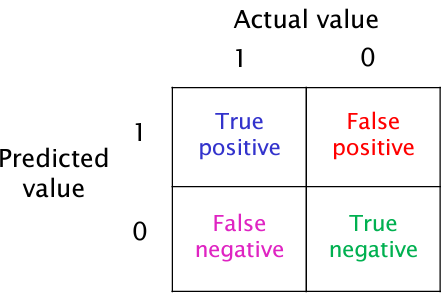
\includegraphics[scale=0.7]{img/confusion.png}
\end{figure}
\noindent
Based on the data collected in such a matrix, we can compute two different metrics: \textbf{precision} and \textbf{recall}. The former answers to the question: "Of all patient we predicted $y=1$, what portion has actually cancer?", the latter "Of all patients where we predicted $y=1$, what portion we did we correctly estimate?". In formulas:
\begin{equation}
    \text{Precision}(p)=\frac{TP}{TP+FP}\quad
    \text{Recall}(r)=\frac{TP}{TP+FN}
\end{equation}
In order to compare such metrics, another auxiliary index is introduced, the $F$ Score which is the armonic mean between recall and precision:
\begin{equation}
    F\text{-score}=\frac{pr}{p+r}
\end{equation}
Other metrics can be used, for example the \textbf{average of the diffenent accuracy indexes} in some situation can make sense, in other different situations also \textit{handcrafted} metrics can be used. It is remarkable that whether we want use eterogeneous metrics it is adviceable to maximize/minimize a single index while having the others as constraints (eg. \textit{maximize \textsf{Accuracy} subject to \textsf{Running time}$\le$100 ns})

\section{Human-level performance}
Sometimes can be useful what is the error that a human do in a classification task in order to understand on what to put the focus (ie. High-bias or high-variance or both), moreover other statistical error-rate can be computed as the \textbf{Bayes Error} which is the \textbf{lowest possible error-rate} for a given classifier. The \textit{Bayes Error} in some situation can be higher with respect to the \textit{Human-error}, this becuse by properly training a neural network the model can have the experience of several humans. Let us give an example:

\begin{figure}[h]
    \centering
    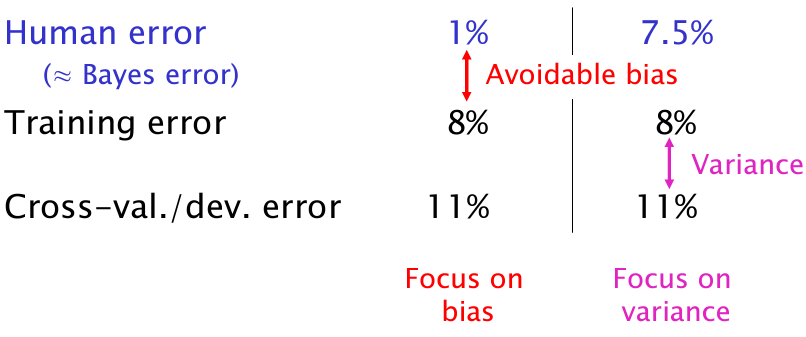
\includegraphics[scale=0.7]{img/performances.png}
\end{figure}
In the first case we can note that there is a bigger difference between the Human and Training error (here is assumed to be very similar to the Bayes error) than the one between training and validation error $\to$ we have to focus ourselves on the bias and use some strategies in order to reduce it. (This is an avoidable bias since it is mostly sufficient making the model grow to eliminate it).\\
In the second case we have similar human and training error, while there is an higher difference between the training and validation error. The most desireable thing is orthogonalize such properties which implies \textbf{having small bias while keeping low variance}, so we want them not to influencing each other (in this  sense \textit{orthogonal}).

\section{Facing bias and variance}
From a study of 2001 it appears evident that:
\begin{quotation}
    "It's not who has the best algorithm that wins, it's who has the most data" (Banko and Brill, 2001)
\end{quotation}
In principle:
\begin{itemize}
    \itemsep-0.2em
    \item In order to \textbf{reduce the bias} could be sufficient to have a \underline{\textbf{bigger model}}; 
    \item In order to \textbf{reduce the variance} could be sufficent to \underline{\textbf{use more data}} in the training phase of the model.
\end{itemize}
From a conceptual point of view it is sufficient to use the following flow-chart:

\begin{figure}[h]
    \centering
    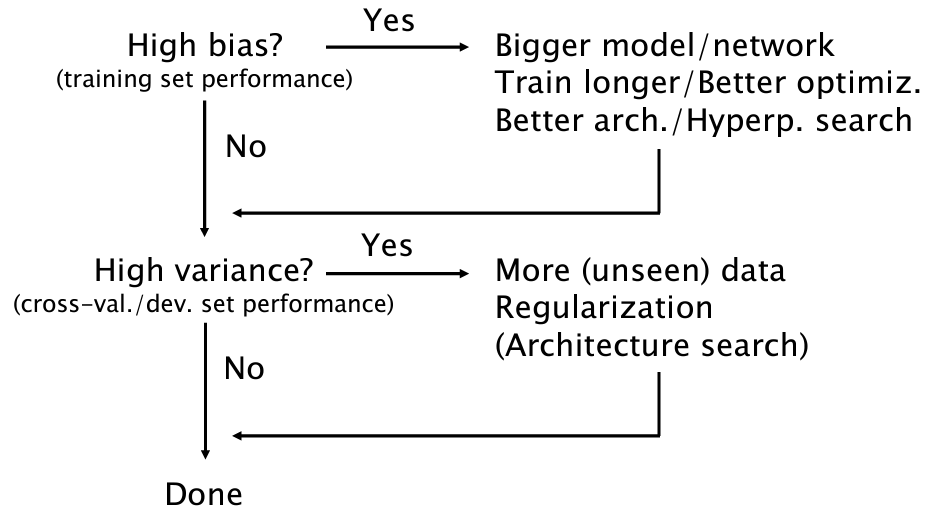
\includegraphics[scale=0.5]{img/flowchart.png}
\end{figure}
\noindent
The real-world examples demonstrates that variance and bias cannot be orthogonalized, then there is a \textbf{trade-off} to manage.


\chapter[Large Datasets and Big models]{Large Datasets and Big Models}

\section{Why deep networks?}
Several studies have demonstrated that for certain task the performance of certain machine learning models are better with the increasing complexity of the model working on the same set of data. That is when you have a huge amount of data more complex models have better performances. 
The graph showed below explains such a feature:
\begin{figure}[h]
    \centering
    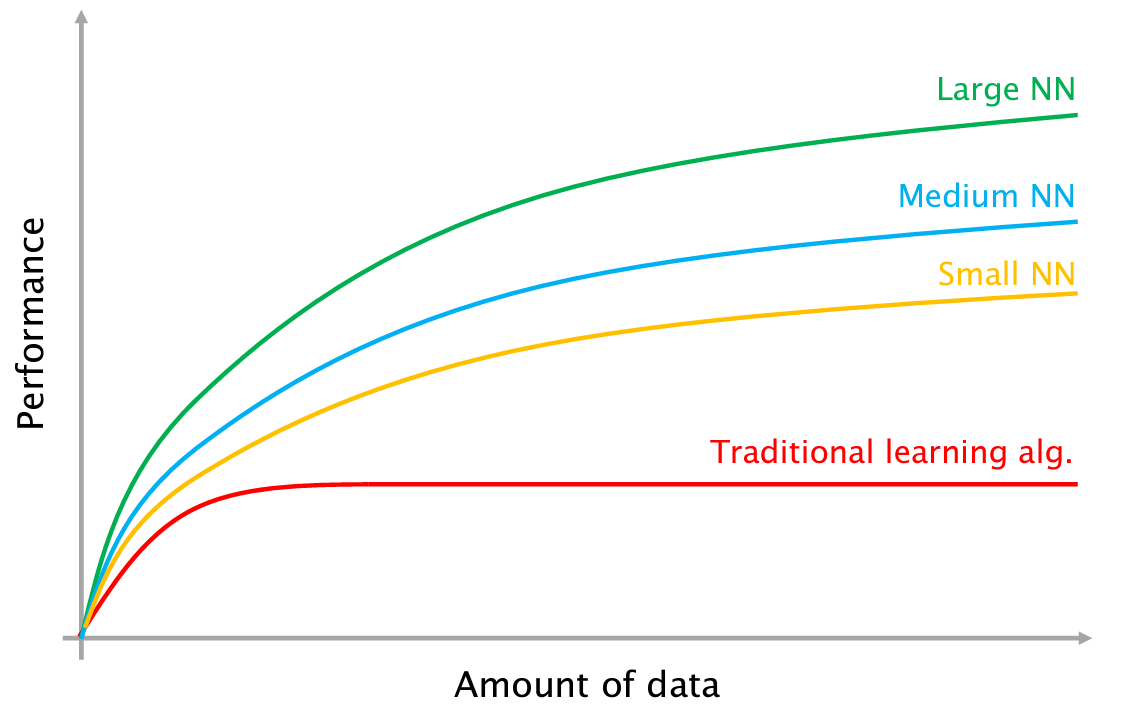
\includegraphics[scale=0.4]{img/perf.png}
    \caption{Amount of data vs Performances varying the model}
\end{figure}
The classical example can be done is the following: imagine that a classification task on images have to be performed, especially whether the figures are colored, there is an exploding number of features. A classical fully connected neural network has very bad performance with respect to a deep network, for example a \textit{Convolutional Neural Network}.

\section{Aspects related to large datasets and deep networks}
We have seen in the past chapter, when a neural network has to be trained there is always a thread-off between bias and variance to manage. There are several aspects related to deep models which ought to be taken into account. In the following the most important aspects are presented.

\subsection{Regularizing neural networks}
How we mentioned in the past paragraphs, the \textit{regularization} is a technique which is used to face the problem of overfitted models. Such a technique consists of introducing into the \textit{cost function} $J(w,b)$ a term which depends on the parameters.
For a single neuron the loss function is modified as follows:
\begin{equation} \label{eq:l2reg}
    J(w,b)=\frac{1}{m} \sum_{i=1}^{m} {\text{Loss}(\hat{y}^{(i)}, y^{(i)})+
    {\color{red}\frac{\lambda}{2m}{\Vert w \Vert_2^2}}}
\end{equation}
The term in red is the \textbf{regularization term}, its effect is to keep the complete set of features without eliminate nothing, the difference is that for certain parameters (associated to certain features) the magnitude is very small or equal to zero in order to reduce in some way the complexity of the model which was causing the overfitting phenomenon. The one showed in the (\ref{eq:l2reg}) is the $\ell_2$-norm regularization, since the $\ell_2$-norm of the vector $w$ of the weights multiplied by a parameter $\lambda$ (regularization parameter) is added to the original functional. Other types of regualarizations can be used for example the $\ell_1$-norm. The regularization term, then has the hyperparameter $\lambda$ which is crucial. In particular:
\begin{itemize}
    \itemsep-0.3em
    \item $\lambda$ \textit{very small} is associated with an \textbf{almost full model}; 
    \item $\lambda$  \textit{very high} is associated with a model whose parameters are very small, and so to a very simplified model.
\end{itemize}
For a neural network of $L$ layers the $J$ functional becomes:
\begin{equation}
    L(W^{[1]}, b^{[1]}, W^{[1]}, b^{[2]}, ...)=\frac{1}{m} \sum_{i=1}^{m} {\text{Loss}(\hat{y}^{(i)}, y^{(i)})}+
    {\color{red}\sum_{l=1}^{L}{\Vert{W^{[l]}}\Vert_F^2}}
\end{equation} 
Where {$\Vert{W}\Vert_F^2$} is the \textit{Frobenius Norm} which is the generalization of the $\ell_2$-norm in the case of matrices. Intuitively the goal is obtaining $\Vert{W}\Vert_F^2$ close to zero, since near the origin the $g(z)$ behaves in a linear way, this avoids the data to be overfitted.\\
Clearly, since $J$ is modified, also the gradient descent is modified. More specifically a term 
\begin{equation*}
    \frac{\lambda}{m} W^{[l]}
\end{equation*}
is added. This results in the update step, in multiplying the weights by a quantity equal to 
\begin{equation*}
    1-\alpha\frac{\lambda}{m}
\end{equation*}
the the higher $\lambda$ the lower such a contribution which shrinks the parameters more and more near to the origin. This is the reason why the $\ell_2$-norm regularization is also called \textit{weight decay}.

\subsection{Dropout}
\textbf{Dropout} is another regularization technique in which for each layer of the network a certain threshold is fixed and this is associated to the probability of keeping or removing one or more of its neurons. The reason why such an apparently strange technique works very well is that removing some units from each layer according to the fixed probability the structure of the network is simpler resulting in a reducing in the overfitting entity. The dropout has to be disabled in the test phase, because is something of helpful only in the phase of construction of the model.

\subsection{Data augmentation}
Among the techniques to reduce overfitting \textbf{data augmentation} is used when the dataset is not so rich. This helps us in obtaining new data starting from the ones in the original dataset. Some distortion are introduced in a way that the model perceives that information as different ones. In the field of image classification this is a very used technique. More specifically when Convolutional Neural Networks grew larger in the 90s, there was a lack of data to use, especially considering that a portion of the dataset was devoted to the testing phase. It was proposed to \textit{perturb existing data} with \textit{affine transformation}, in order to create new examples with the same labels. The most common transformation are: geometric, color space transformation and a sort of noise injection. In the following two examples  are showed with a cat image and with a number.

\begin{figure}[h]
    \centering
    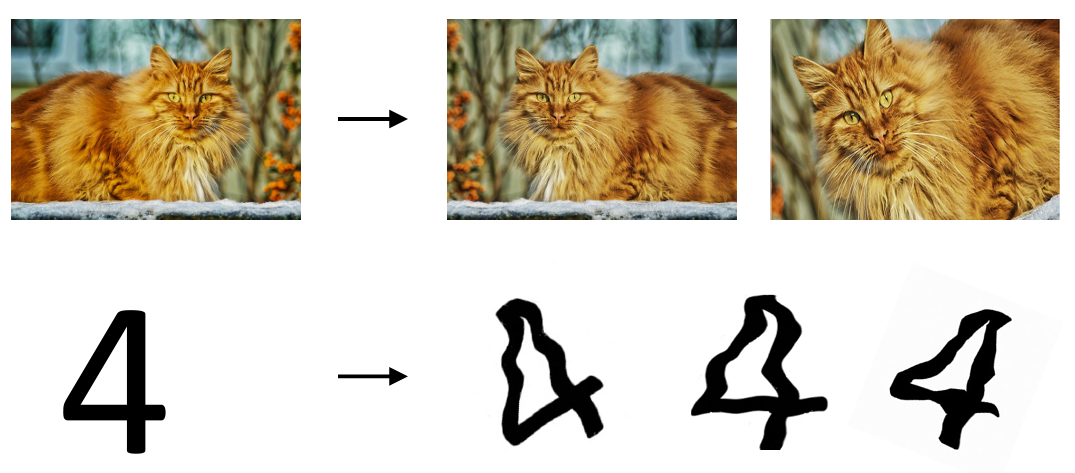
\includegraphics[scale=0.5]{img/data_sug.png}
    \caption{Data augmentation }
\end{figure}

\subsection{Mini-batch gradient descent}
Especially for bigger models than a classical multi-layer perceptron using the "classical" gradient descent could be very slow, since for each one the iterations, which hopefully, bring to the convergence, the \textbf{entire dataset} is scanned. This would have made the procedure very slow! That we called "classical Gradient Descent" is also known as \textbf{Batch Gradient Descent}.\\
The alternative here is to split the entire batch of data constituting the dataset into \textbf{mini-batch}. Doing in this way, one step of Gradient Descent passes through a subset of the data making the computations faster. When all of the batches of the training set have been used an \textbf{epoch} has been completed. In the classical approach one epoch is associated to one step of gradient descent, on the other hand if we split the dataset into $M$ batches, $M$ gradient steps are done in one epoch.

\subsubsection{Loss function and mini-batch gradient descent}
It is not supposed to be a surprise if we state that the shape of cost function through the different iterations is not so smooth as in the \textit{batch version}, since at each step different data are used.

\begin{figure}[h]
    \centering
    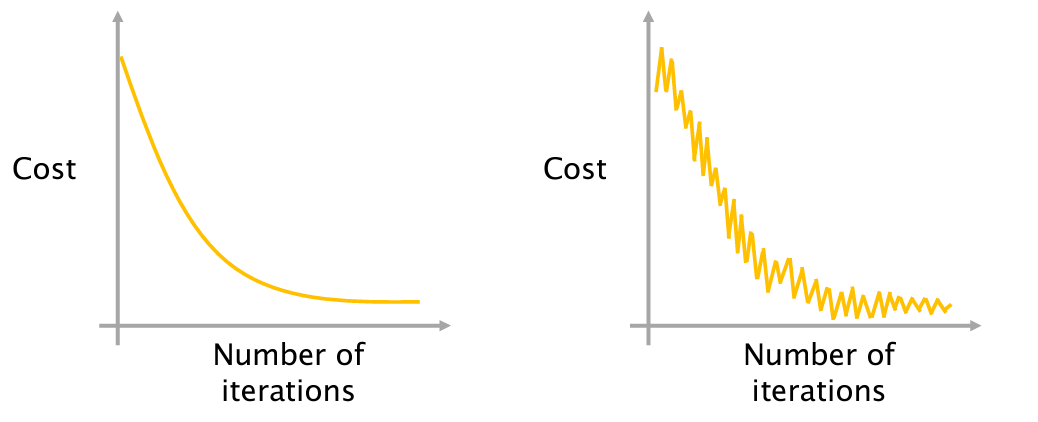
\includegraphics[scale=0.4]{img/mini-batch-iterations.png}
    \caption{\# of iterations vs Cost (Batch vs Mini-Batch)}
\end{figure}

\subsubsection{Mini-batch size}
In the case the size of a mini-batch is 1, we talk about the \textbf{stochastic gradient descent} ot the opposite if the batch size coincides with the cardinality of the dataset, then batch GD = mini-batch GD. If we go deeper into this aspect by analysing the level curves that from the initial conditions bring us to the minimum, the case of batch gradient descent is the ideal one since the path from the initial value to the minimum is straight. The same does not occur in the case SGD is used. In the practical case a value for the mini-batch size between 1 and $m$ must be chosen, this choice results in another \textit{hyperparameter}.

\begin{figure}[h]
    \centering
    \subfigure[size=m]{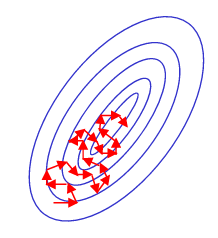
\includegraphics{img/minibatch_contourplot.png}} \quad 
    \subfigure[size=1]{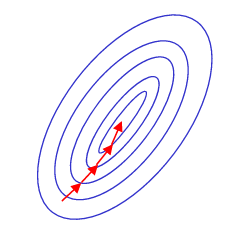
\includegraphics{img/batch_contourplots.png}}
    \caption{Contour plots varying batch size}
\end{figure}

The suggestion in this field is to use the original version of gradient descent with a small dataset (eg. 2000 examples), otherwise typical sizes for mini-batches are 64, 128, 256 and so on. In order to avoid problems, you are supposed to be sure that it fits in the used CPU/GPU.

\subsection{The problem of local minima}
Let us make another objection on the cost function, we have seen which is a fundamental building block of our machine learning task. Now, after having combined the several layers of the network (each one of the layers use different activation functions) is the $J(w,b)$ convex? The answer is NO. The functional we obtain loses its convexity with the increasing complexity of the network. However, thanks to the structure of the final cost function, the probability to be trapped into a local optima is very low. \texttt{part to be rewiewed}

\begin{figure}[h]
    \centering
    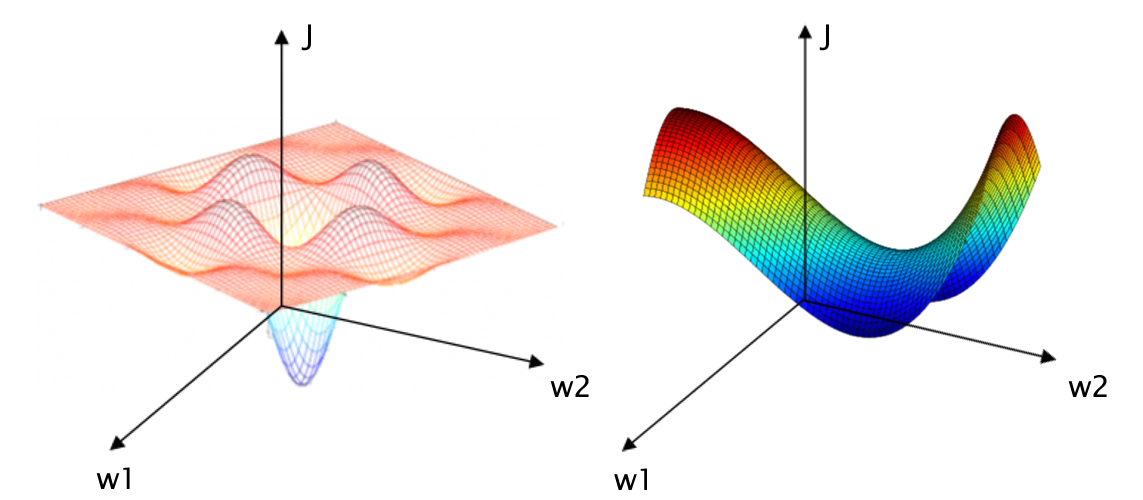
\includegraphics[scale=0.6]{img/Jnocvx.png}
    \caption{Cost function for a NN with two parameters}
\end{figure}
In the case that in the functional there are \textbf{plateaus} can be a problem, since being the derivatives constant the learning is very slow.

\subsection{Exploding/Vanishing gradients and initialization in DNN}
The \textbf{exploding} and \textbf{vanishing gradient} are both problems related to very deep networks were the weights are too high or too low, in the former case the computed gradients \textit{grow exponentially}, in the latter case they decrease their own value till they become null.\\
For sake of simplicity suppose that the activation function is a line $g(z)=z$, moreover let $b=0$, than the predicted output $\hat{y}$ has the shape:

\begin{equation*}
    \hat{y}=W^{[L]}W^{[L-1]}...W^{[1]}{x}
\end{equation*}
Whether for example the weights were all equal to 1.5 the $\hat{y}$ would be very big, on the other hand, whether all of the weights were 0.5 there would be an \textit{exponential decreasing} of the activations, a similar situation occur for the derivatives. In deep neural networks not rarely such problems appear, and differently from the \textbf{shallow neural networks} a more accurate technique aimed to cope with them is needed. In particular, has been empirically demonstrated that such a problem is reduced when the weights $w^{[l]}$ of a certain layer $l$ are randomly initialized with a value in the range $[0,1]$ multiplied by the standard deviation
\begin{equation*}
    \sigma^{[l]}=\sqrt{\frac{1}{n^{[l-1]}}}
\end{equation*}
where $n^{[l-1]}$ is the number of unit of the $(l-1)$-th layer (previous layer).


\subsection{Batch normalization}
We have seen in the introduction in order to speedup the training phase a proper choice when data are on completely different scales is the \textbf{normalization}. To better clarify such an aspect, we can say that 2 different steps are performed\footnote{
    The same $\mu$, $\sigma$ are supposed to be used in order to normalize also the remaing parts of the dataset: \textit{test} and \textit{development} set.
}:
\begin{itemize}
    \itemsep-0.3em
    \item Subtract the mean $\mu$ computed on that feature on the whole dataset (to be computed a-priori); 
    \item Divide by standard deviation $\sigma$ computed always over the whole training set for that specific feature.
\end{itemize}
In the past years, scientists working on deep learning has showed that if such a normalization is applied also for the activations (more specifically to the linear part $z$), then the learning of the parameters for a certain level is \textbf{faster}. This is the main feature behind the \textbf{batch normalization}. We know that for a certain layer $l$, we can compute the activation $A^{[l]}$ as:
\begin{equation*}
    A^{[l]}=g(Z^{[l]})
\end{equation*}
then the \textit{batch normalization} procedure is carried out as follows:
\begin{itemize}
    \itemsep-0.3em
    \item For each layer $l$, for each feature $i$, the mean $\mu$ and variance $\sigma^2$ are computed.
    \item The normalized data $Z^{[l](i)}_{\text{norm}}$ are obtained as follows:
    \begin{equation*}
        Z^{[l](i)}_{\text{norm}}=\frac{
            Z^{[l](i)}-\mu
        }{
            \sqrt{\sigma^2+\varepsilon}
        }
    \end{equation*}
    \item For the training phase the following data are used:
    {\large{
        \begin{equation}\label{eq:batch_normalization}
            \tilde{Z}^{[l](i)}={\color{red}\gamma}{Z}^{[l](i)}_{\text{norm}}+{\color{red}\eta}
        \end{equation}
    }}
\end{itemize}
This approach, fortunately or not, leads with it other hyperparameters which are $\varepsilon, \gamma, \eta$. Moreover, just to further complicate the situation, for each layer different $\gamma^{[l]}$ and $\eta^{[l]}$ could be used. It is interesting now, after this formal description to better understand what are the guidelines leading to batch normalization and what is its effect. \\
In principle when I perform the normalization on the input data (remind they are also called 0-layer activations) after the first forward step, I completely lose the effect since the first-layer activations are something very different than the \textit{normal} range. Moreover batch normalization also has a \textit{slight regularization effect}: the fact that mean and variance are computed with respect to that mini-batch adds similarly than \textit{dropout} adds some noise to each hidden layer activations. 

\subsection{Softmax Layer}
At the beginning we have seen that the hypotesis (later called \textit{activation}) can be interpreted as the probability of belonging to a certain class given the records X, but how can be interpreted as a result? We would like to have on the last layer $L$ a some probability that, differently from the other sum up to one. For this reason, very often in the neurons of the last layer a particular activation function is used: 
\begin{equation} \label{eq: Softmax}
    a_i^{[L]}=\frac{t_i}{\sum_{j=1}^{n^{[L]}}{t_j}}
\end{equation}
where $a_i^{[L]}$ is the activations for the $i-th$ unit in layer $L$, and $t_i\doteq{e^{z_{i}^{[L]}}}$. When the softmax activation function is used, the loss function to be used is the following (\textit{for a single training sample}): 
\begin{equation}\label{eq:loss_softmax}
    \text{Loss}^{(i)}(\hat{y}, y)=\sum_{j=1}^{n^{[L]}} -y_{j} \log(\hat{y}_j)
\end{equation}
Note that $n^{[L]}$ is the number of classes, in this case for the $m$ training samples the \textbf{one-hot encoding} is used for representing the labels, in particular:
\begin{equation}\label{eq: one_hot}
    Y=\big[
        y^{(1)} \quad y^{(2)} \quad ... \quad y^{(m)}
    \big] = \begin{bmatrix}
        0&1& &0\\
        1&0& &1\\
        0&0&...&0\\
        0&0& &0
    \end{bmatrix} \in \mathbb{R}^{n^{[L]}, m}
\end{equation}
For each example a vector in which only $i$-th element is one with correspondence to the true class for that record.

\subsection{Transfer learning}
Especially in the field of deep learning, rarely one starts from scratches to develop the neural network. There are several motivations for which this is not happening, a common one is that there is lack of resources. To the aim to train certain models several dozens of GPU could be required... The \textbf{Transfer learning} aids us to cope with this problem. It consists in the use of a part of a pre-trained model in order to use its parameters as input features for a task of us. Then, by doing the so called, \textbf{surgery of the network} several layers are freezed,in the sense that only the forward step is done on these, while the parameters are updated only for the few last layers. The difference is that if we had started from scratches a lot of time and hardware/software resources would have been needed. This is one of the best common practice of the deep models.\\
\textbf{Can we always use transfer learning?} The answer is clearly No! You can pass by this procedure: either when two tasks have common inputs, or you have more data for a task then for another, or also low level features for a task could be useful for the other.
\chapter[Computer vision and CNN]{Computer vision and Convolutional Neural Networks}

\textbf{Computer Vision} is a field of Artificial Intelligence which aims to implement models that performs visual tasks. Some of the tasks in this field are for example: \textit{image classification}, \textit{object detection} within an image, the so-called \textit{neural style transfer} and so on. All of this tasks, for the nature of input data, involves an enormous number of features which corresponds to a huge number of parameters to learn. How we have said several times, a \textit{classical neural network} (shallow) for example, cannot perform properly and in acceptable time such a task. Just for give an idea, the number of parameters to lean can be also around a billion! For this reason \textbf{convolutional architectures}, and then \textbf{convolutional neural networks} are introduced.

\section{Convolutional Neural Networks: main ingredients}
A \textbf{Convolutional  Neural Network} (\textbf{CNN}) is made up of several parts: (i) a \textit{convolutional layer}, (ii) a \textit{pooling layer}, (iii) a \textit{fully connected layer}.

\subsection{Convolution}
This is the core building block of a CNN, here the great majority of the computation occurs; there are several levels of this type. Besides, the convolutional layers are the ones in which the network learns the main feature from the input data. In the case of images, passing through the convolutional part of the NN low level to high level features are learned. The following figure shows an example of the extracted details at different levels of the architecture:

\begin{figure}[h]
    \centering
    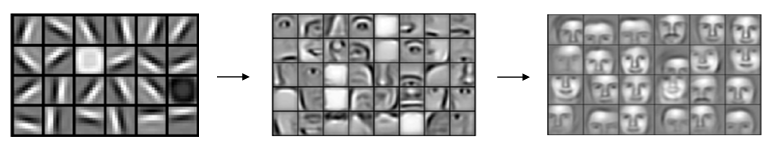
\includegraphics[scale=0.8]{img/CNN_example.png} 
\end{figure}

\noindent
You can see in the first stage only some edges are detected, passing through more complicate details arriving to the detection of entire faces. \\
This procedure takes inspiration on how our brain solve the problems; biological studies have confirmed that in order to perform a certain task, our brain solves, step by step, simpler problems in order to reach more complicate ones.\\
From now on, we are going to focus our attention on \textbf{images}, and in particular we are going deeper in some details on \textit{how convolution process works}.\\

The \textit{convolution} requires few components: (a) input data, (b) a \textbf{filter}, (c) a \textbf{feature map}. Considering that an image can be seen as a matrix of pixels, roughly speaking the filter moves across the image checking if the feature for which that filter itself has been built, is present. This process is known as \textbf{convolution}.

In the following there is a figure that shows, mathematically speaking, what are the main steps behind such a procedure.

\begin{figure}[h]
    \centering
    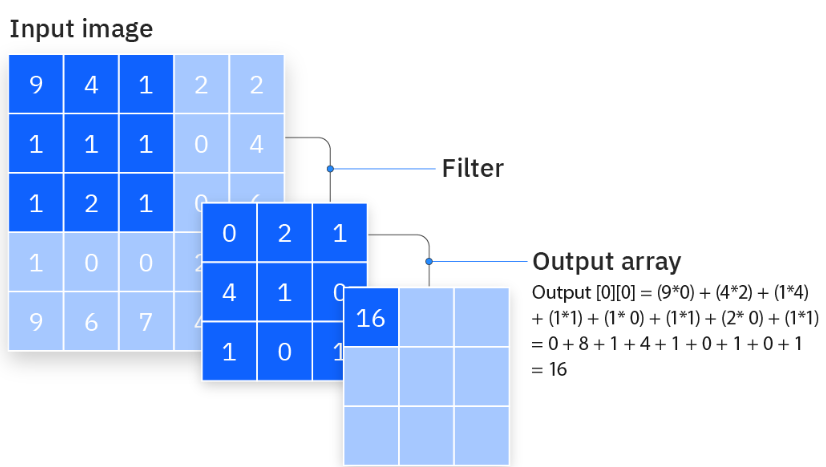
\includegraphics[scale=0.8]{img/convolution.png}
    \caption{Convolution: main steps}
\end{figure}

\noindent
In practical terms also a filter is a square matrix (with \textit{odd dimension}) in a way that it has a center. Such a filter is \textit{convolved} to the image in the sense it slides across subregions of it which have the same dimension of the feature detector; the output array (another matrix called the \textbf{feature map}) is done by scalars corresponding to the sum of the product element by element of the involved matrices. \\
How we will see, part of the parameters that the the network has to learn are those constituting such filters, then no one tells to the network how to find edges (also at different inclination) or other types of details!\\
 It should be clear that, going across the process of convolution the dimension of the matrices is reduced. In particular: starting from an image (square for simplicity) $n\times{n}$, by applying on it a filter $f\times{f}$ the dimension of the ouput will be shrinked by a quantity $f-1$ (for each dimension), with a resulting size of $(n-f+1)\times{(n-f+1)}$.

\subsubsection{Padding}
We can add a frame of padding to the image (usually by adding zeros) in order to avoid the phenomenon of \textit{shrinking dimensions}. Then, if a padding of $p$ is added to the input image (so that it results in being $(n+p)\times(n+p)$) and an $f\times{f}$ filter is applied the resulting image will have shape $(n+2p-f+1)\times{(n+2p-f+1)}$.

%%TODO: Uso il padding anche perché altrimenti perderei delle informazioni ai bordi dell'immagine

\begin{figure}
    \centering
    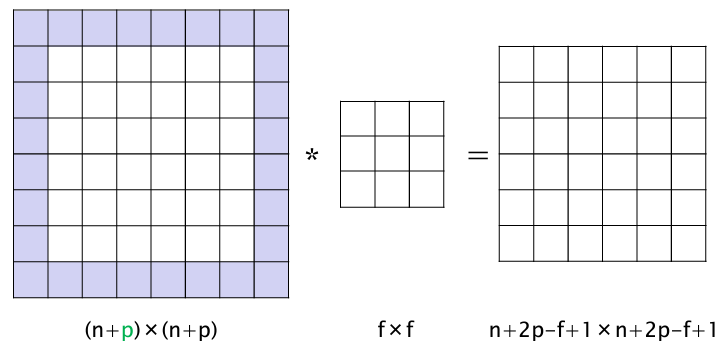
\includegraphics[scale=0.6]{img/CNN_padding.png}
    \caption{Image padding for avoiding dimension reduction}
\end{figure}

Only for a matter of nomenclature, we have to say that a convolution which does not use the padding is called \textit{valid convolution}, otherwise we have a \textit{same convolution}. The \textbf{amount of padding} to be added is such that the input and ouput images have exactly the same shape. By doing simple calculations we can find that this quantity is equal to $p=(f-1)/2$, it gives always a non-fractional value since $f$ is known to be odd.

%Attenzione qua: s=1 vuol dire nessun pixel saltato (mi sposto di uno ogni volta cioè non salto nulla)
\subsubsection{Strided convolutions}
The last step is needed to complete the overview on the first part of CNN: \textbf{strided convolutions}. Whether in the procedure of applying the kernel some pixels (cells of the matrix) are skipped, then the procedure is known to be \textbf{strided}. A number of skipped cells greater than one is rare, however it is remarkable that also in this case the dimension of the feature map is shrinked. More clearly, for a stride $s$ the dimensions for the output are: 
\begin{equation*}
    \left\lfloor \frac{n+2p-f}{s}+1\right\rfloor\times
    \left\lfloor \frac{n+2p-f}{s}+1\right\rfloor
\end{equation*}
How you will imagine, after some chapter of discussion on NN, such an $s$ is another hyperparameter (usually $s=1$, if a \textit{same convolution}) is used.

%TODO: Quando le dimensioni non sono sufficienti certe combinazioni vengono saltate (per convenzione). Qui l'obiettivo è quello di ridurre la dimensione dell'output al contrario del padding.

% Convoluzione --> combinazione lineare
% Padding --> Mantenere dimensione output
% Strided convolution --> Ridurre output

\subsection{Convolutions on RGB images}
In the previous paragraphs, for sake of clarity about the main aspects of convolution, we have implied that the image for which we were training the CNN was a gray-scale one. A part from few tasks, nowadays colored images are used.
Let us suppose, without loss of generality, on the contrary they are RGB ones. This implies that now the input images are not 2D-arrays anymore, they are 3D since there is an $n\times{n}$ matrix for each one of the three channels R, G, B. A \textit{3D-kernel} is needed as the number of channels. Despite the shape of the inputs is changed, what is not changing is the simple computational procedure, since all of the values are summed up! Then the feature map is always a 2D-array and the network is clearly allowed to use different or same filters. 

\subsubsection{Multiple Filters}
In the case that at this stage \textit{multiple filters} are used, also the output has a three-dimensional shape.
Now, whether on a RGB image whose shape is ${n}\times{n}\times{n_C}$, is applied $n_C'$ (number of channels of the output) filters whose shape is ${f}\times{f}\times{n_C}$ (with $n_C$ being the number of channels) $\to$ the output shape will be (no padding, no striding) $(n-f+1)\times(n-f+1)\times{n_C'}$.\\

\begin{figure}[h]
    \centering
    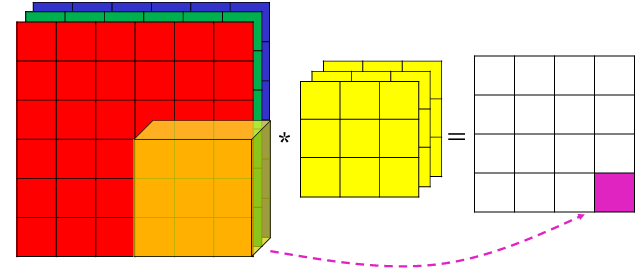
\includegraphics[scale=0.6]{img/CNN_RGB.png}
    \caption{Convolution on RGB images producing 2D-output}
\end{figure}

We can see that the convolution operation is nothing but a (just more complicated) linear combination. This is the counterpart of $z$ in the linear regression, then -- also here -- a \textit{nonlinear part} is missing! In fact, before passing the output to the next layer, even in this case an activation function is employed, in particular the ReLU. This prepares the activations for the next layer. Such a situation is well depicted in the following:

\begin{figure}[h]
    \centering
    \includegraphics[scale=0.7]{img/ReLU_CNN.png}
    \caption{ReLU on feature maps}
\end{figure}

\subsubsection{Example: Number of parameters in a CNN}
How many parameters we have in a layer of a convolutional neural network which use \textit{10 filters} $3\times3\times3$? For a single filter we have:  $3\times3$ parameter for each 'sheet', there are 3 sheets for a filter, then for a single filter we have 27 parameters. Furthermore, there is another parameter for each filter which is related to the bias which is added before passing for the ReLU. Since we have 10 filters, the total number of parameters is 
\begin{equation*}
    (3\times3+1)\times10=280
\end{equation*}

\subsection{Notation}
Here we introduce some notation which will be useful in the comprehension of the examples of CNNs. Suppose we have the $\ell$-th convolutional layer, for such a layer we can have some filters of dimension $f^{[l]}$ (they are square), we could apply some padding and/or stride, respectively $p^{[l]}$ and $s^{[l]}$. Then, the \textbf{input} will have dimension $n_H^{[l-1]}\times{n_W^{[l-1]}}\times{n_C^{[l-1]}}$, while \textbf{the output} will have dimension $n_H^{[l]}\times{n_W^{[l]}}\times{n_C^{[l]}}$, where $n_C^{[l]}$ is the number of filters for the $\ell$-th layer, while $n_{H/W}^{[l]}$ is equal to:
\begin{equation}
    \left\lfloor \frac{n^{[l-1]}+2p^{[l]}-f^{[l]}}{s^{[l]}}+1\right\rfloor
\end{equation}
\textbf{Each filter} has dimension $f^{[l]}\times{f^{[l]}}\times{n_c^{[l]}}$, the dimension for an activation for a certain layer is equal to the output, since we have $m$ examples we have $m$ times the dimension of the output. All of the activations are indicated with $A^{[l-1]}$. The \textbf{number of parameters} for a layer is:
\begin{equation}
    f^{[l]}\times{f^{[l]}}\times{n_C^{[l-1]}}\times{n_C^{[l]}}+n_C^{[l]}
\end{equation}
Note here that a filter has a dimension that is equal to the dimension of the output of the previous layer.
In the following an example is showed in which there are 4 convolutional layers:

\begin{figure}[h]
    \centering
    \includegraphics[scale=0.8]{img/ConvNet_Example.png}
    \caption{Example of a CNN (with all the dimensions)}
\end{figure}


\subsection{Pooling layer: Max-Pooling}
Once also the ReLU has been computed, the output is further modified. A \textbf{pooling function} replaces the output of the net for a certain location with a \textit{summary statistic} of the nearby outputs. The most commons are the \textbf{max-pooling} and the \textbf{average-pooling}. The type of statistic to be used is a user-defined choice. The introduction of pooling bring with itself other two hyperparameters, the dimension of the \textit{neighbourhood} on which the pooling is applied, the stride by which this occurs.

\begin{figure}[h] \label{fig: CNN_example}
    \centering
    \includegraphics[scale=0.7]{img/MaxPooling.png}
\end{figure}

In this case the added hyperparameters are $f=2$ (dimension of the sub-blocks) and $s=2$ since at each pooling stage a cell is skipped. \\
Clearly the pooling reduces the dimension of the activations, but it is useful in order to summarize the information obtained at a certain stage. It is remarkable that different than the convolution stage, the pooling stage is performed separately for each channel of given activations.

\subsection{Fully connected layer}
The convolutional layers -- made up of convolutional and pooling stage -- works as feature extractors, finally at the end of the architecture some \textit{fully connected layers} are present, they carries out the work of classifying a given example, then the last layer is a \textit{softmax} one, which gives for each class a probability for the sample to be part of a certain class. 
Look at the Figure (\ref{fig: CNN_example}), for the last  volume if we isolate a single cell, this is nothing but a linear combination of the parameters plus a bias, this is a neuron! Then the first fully connected (Dense) layer is nothing but the unrolling of all of the neurons contained in the last volume.\\

\noindent
As first example, the CNN for the \textit{digit classification is given} (see \cite{lenet5} for further information):

\begin{figure}
    \centering
    \includegraphics[scale=0.7]{img/LeNet_digit.png}
    \caption{\textbf{LeNet-5}: CNN for digit recognition}
\end{figure}
Note how the pooling stage does not change the third dimension (the depth of the volume) but only the height and width. As usual the last volume from POOL2 is unrolled in some computational units which made up the first layer for the fully connected part of the network. \\
In the pooling stage there are no learned parameters since only a statistic summary is done on subregion of the activations.

\subsection{Why Convolutions?}
The convolutional stage is very used, mainly for two aspects: 
\begin{itemize}
    \itemsep-0.3em 
    \item \textbf{Parameter sharing}: when a filter for a part of the image is used (eg. edge detection) probably it will be useful also for another part of the image; the same parameters used for different part of an image and (why not) for other images in which the same low/high level features, could be detected.
    \item \textbf{Sparsity of connections}: at each layer the outputs depend on a small number of inputs.
\end{itemize}
It could appear strange, but in a CNN the great majority of the parameters are concentrated in the fully connected layers! This is one of the reason why shallow fully connected networks performs very bad in terms of image classification.

\section{Case studies and tasks}
In the following some examples of CNN architectures are reported, for sake of completeness also the paper are cited.

\subsection{AlexNet}
This type of architecture was introduced in \cite{AlexNet}, and the objective was the image classification, differently from \textit{LeNet-5} having 2 convolutional layers, this architecture contains 6 convolutional layers. The depth of the network was relevant for the obtained results which opened the road to a lot of studies on computer vision. The AlexNet paper is one of the most cited ones especially for the obtained results. Just for give an idea, the training set had 1.2 million images. It was trained for 90 epochs, which took five to six days on two NVIDIA GTX 580 3GB GPUs which had been working in parallel. 

\begin{figure}[h]
    \centering
    \includegraphics[scale=0.6]{img/AlexNet.png}
    \caption{\textbf{AlexNet} architecture}
\end{figure}

\subsection{VGG-16}
They are named after the \textit{Visual Geometry Group (VGG)} of the Oxford University. The full description of the net can be found in \cite{VGG-16}. 16 is the number of its layers (13 convolutional, 3 deep), there are other VGG networks with a different number of layers.

\begin{figure}[h]
    \centering 
    \includegraphics[scale=0.5]{img/VGG16.png}
    \caption{\textbf{VGG-16} architecture}
\end{figure}

\subsection{Residual Network(ResNet)}
Till now we have mentioned the structures of the DNN \textit{LeNet, AlexNet, VGG-16}. In a similar way we could build up our deep neural network, ma in the practice they are hard to train. Residual Networks allow us to perform a more efficient training of them. \\
We have seen in the previous paragraph that DNNs suffer the problem of the \textit{vanishing gradient}, we can say that data is disappearing through the network. Some reaserchers from Microsoft found that the split of a deep network into chuncks help eliminate much of this disappearing signal problem. In other words \textit{ResNets} breaks down  a very deep plain neural network into \textbf{small chuncks of network} connected each other by using \textit{skip} or \textit{shortcut connections}.


\begin{figure}[h]
    \centering
    \includegraphics[scale=0.5]{img/ResNet.png}
    \caption{\textbf{ResNet} skip connections}
\end{figure}
\noindent
In the figure above we can see the core constituting ResNets: \textbf{skip connections}. Roughly speaking the activation of the layer $l+2$ are computed using also the activation from the layer $l$. In this sense there is a skip through the layers. On such a type of architecture we have that the training error curve is how we can expect from the theory, differently from the \textit{plain neural networks}. In the following we show an example of ResNet with 34 layers in which \textit{skip connections} are used. The number of layers skipped is two, but "very surprisingly" the number of skipped layers can become another hyperparameter. In the original case presented in \cite{ResNet} the skip connection is from the level $l\to{l+2}$, that is the activation of the level $l$ influences the ones in the level $l+2$.

\begin{figure}[h]
    \centering 
    \includegraphics[scale=0.6]{img/ResNet2.png}
    \caption{Example of 34-layers ResNet}
\end{figure}

\section{${1}\times{1}$ convolutions}
We have seen that in the convolutional stage some filters are applied in order to produce a linear combination of the input data. Could be strange, but there are some cases in which doing a $1\times{1}$ convolution is useful in order to reduce the number of computations, since the number of multiplications is directly proportional to the dimension of the filter! \\
Now, suppose we have an initial volume as the one represented in blue and we apply a filter as the one in yellow, we are doing nothing but the computation that occurs in a neuron (a part from the ReLU which is performed at the end): the $1{\times}{1}\times{32}$ filter applied to the volume gives us a linear combination of the input at the same Height and Width, but on different channels through the parameters contained into the filter. This is the reason why such a type of procedure is called \textit{Network-In-Network} (see \cite{NetInNet} for further details), this clearly reduces the number of multiplications that are performed.

\begin{figure}[h]
    \centering
    \includegraphics[scale=0.6]{img/NiN.png}
    \caption{Network-In-Network and $1{\times}{1}$ convolutions}
\end{figure}


\subsection{Inception: another DNN architecture}
From the ideas presented in \cite{NetInNet} and with the increasing in computation capabilities, in Google was created a new CNN architecture who has been called \textbf{Inception} (see \cite{Inception}) (from a famous film from which they was inspired, in particular by an iconic phrase appeared in a meme \textit{"We need to go deeper"}). Such a network has 22 layers, the great majority of them are inception modules, which are a culmination of the results presented in \cite{NetInNet}. Such an CNN is one the most used  architecture in computer vision.

\begin{figure}[h]
    \centering
    \includegraphics[scale=0.3]{img/InceptionModule.png}
    \caption{An Inception Module}
\end{figure}

\noindent
In an \textit{inception module} some $1{\times}{1}$ convolutions are used in order to reduce the number of computations of a 10 factor.
The main motivation behind the Inception modules is that DNN performs better if the number of layers is increased (that is the dimension of the network is increased).\\

\noindent
At the end of this discussion about DNN a graph in which the perfromances of the presented architectures is compared to the \textit{human/Bayes error}. 

\begin{figure}[h]
    \centering
    \includegraphics[scale=0.5]{img/PerfDNN.png}
    \caption{DNN performances vs human error}
\end{figure}

\section{Other computer vision tasks}
Till now we have introduced the main architectures of CNN, we have discussed the basic operations behind them as convolution and pooling. Beyond the classification task there are other more complicate tasks such as object detection, segmentation and semantic segmentation, human-pose recognition and so forth. There are other tasks that combine computer vision to language processing (see for example the \textit{Image captioning}).\\

At the very beginning of this notes we have seen that the idea of \textit{artificial intelligence} is not new at all! But today we are having an increase in the amount of data and computational capability that is favorable for the Machine Learning growth. Just to give an idea the architecture \textit{LeNet-5} was trained on a computer with $10^6$ transistors and no GPUs; \textit{AlexNet} was trained on GPUs with an availability of $10^9$ transistors (three order of magnitude bigger!) As far as the number of pixels is concerned we are talking about $10^7$ in the first case and $10^{14}$ talking about AlexNet.


\chapter{Beyond image classification: Object Detection}
\chapter[Segmentation and Neural Style Transfer]{Beyond classification and detection: Segmentation, Instance Segmentation,  Neural Style Transfer}

\begin{quotation}
    \noindent
    \textsf{In this chapter we will consider other, even more  complex, computer vision tasks including \textit{semantic segmentation} (the task of classifying each pixel of an image) here encoder-decoder architectures are used, \textit{instance segmentation} (combining object detection and semantic segmentation), \textit{face recognition} using Siamese Network and finally the first step toward the world of generative AI concerning \textit{neural style transfer}.
    }
\end{quotation}

\section{Semantic segmentation}
\textbf{Semantic Segmentation} is the task of labeling each pixel within an image with a \textit{category label} without differentiate instances/object of a certain class. Roughly speaking: I know that a certain pixel of a given image is associated to a cow, but I don't know that there is one or more cow in the image itself. \\
Let us introduce this topic by doing an important observation: since I want to classify each pixel of a given image, the size of the output (width, height) is supposed to be the same as the input. \textbf{What approach can we use?} Let us analyze the problem step by step, following the intuition and then introducing more complex reasonings in order to make the architecture scale up. 

\begin{figure}[h]
    \centering
    \includegraphics[scale=0.8]{img/Sem_Seg.png}
    \caption{\textbf{Semantic segmentation} Since here I am not able to separate different instances of a given class, I cannot distinguish two cows within the image on the right}
\end{figure}
In the case we want to perform a \textit{semantic segmentation} we can try to use the sliding window approach classifying the center pixel with a ConvNet. How you can image, this approach is extremely inefficient since the image must pass through an entire pipeline until all of its pixels have been classified, without reusing the shared area among the several patches/window. \\
Now, trying to follow the same path as the object detection, we can go toward a \textbf{fully convolutional approach}, since we have to fulfill the requirement on the shape of the output, one could propose to fix 2/3 of the dimension in a way that \emph{height and width} can have the same shape across the convolutional layers. This solution does not scale on the input size, for this reason new models are used called \textbf{encoder-decoder} that downsample and then \textbf{upsample} in the second part of the network in order to match the input size by using: (i) \textit{in-network upsampling} (\textbf{unpooling}), (ii) \textit{learnable upsampling} (\textbf{deconvolution or transpose convolutions}) (both these aspects are explained in \cite{noh2015learning}).

\subsection{In-Network upsampling: Unpooling}
The \textit{pooling} operation in convolutional networks helps us to filter \textbf{non-robust activation} by keeping a single (max/average...) representative value. However all the spatial information about such a value is lost. In order to solve such an issue the unpooling layer is employed into the deconvolutional part of the network (decoder) is used. The unpooling perform the \textbf{reverse operation of pooling} and reconstruct the original size of activations. Some \textbf{switch variables} are used in order to store the location of the maximum activation as showed in the following: 

\begin{figure}[h]
    \centering
    \includegraphics[scale=0.5]{img/Unpooling.png}
\end{figure}
The first part and second part of such an architecture are simmetric, so that the pooled and unpooled layers are specular. 

\begin{multicols}{2}
    \begin{center}
        \includegraphics[scale=0.5]{img/FCNvsED.png}
        Activation maps from FCN and Encoder-Decoder architecture
    \end{center}
    \begin{center}
        \includegraphics[scale=0.8]{img/Unpool_Deconv.png}
        Pooling/Unpooling and Convolution/Deconvolution
    \end{center}
\end{multicols}

\subsection{Learnable upsampling: Deconvolution}
When the unpooling operation is applied we retrieve an \textbf{enlarged} but \textbf{sparse} map. The main role of the \textit{deconvolutional part} of an encoder is to \textbf{densify the sparse activations} obtained by unpooling. How the \Cref{fig: deconv_unpool} shows, the deconvolution operation maps a single input into multiple outputs. Several \textit{learnable deconvolutional filters} are used which have a similar function with respect to the convolutional one. Lower layers are likely to capture the shape of the overall object while the deeper one will the capture other \textit{fine details}. In this way the decoder \textbf{directly takes class-specific shape information into account}.\\
The \textbf{transpose convolution} operation takes the input feature map and multiply a certain value for all the value contained in the filter so that the important information from the encoder are spread back; in the overlapped region takes as activation the sum of the numbers. In conclusion as in the case of "normal" convolution there are some hyperparameters (filter dimensions and stride).\footnote{Going more deeply, we can say that \emph{"...unpooling and deconvolution play different roles for the construction ot segmentation masks. Unpooling captures \underline{example-specific} by tracing the original locations (with strong activations) back to the image space. As a result, it effectively reconstructs the detailed structure of an object in finer resolutions. On the other hand, learned filters in deconvolutional layers tend to capture \underline{class-specific} shapes. Through deconvolutions, the activations closely related to the target classes are amplified while noisy activations from other regions are suppressed effectively. By the combination of unpooling and deconvolution, our network generates accurate segmentation maps."}(from \citeauthor{noh2015learning} \cite{noh2015learning}).}

\subsection{SegNet: Encoder-Decoder for Image Segmentation}
SegNet (\citeauthor{badrinarayanan2017segnet} \cite{badrinarayanan2017segnet}) introduces a more robust way to segment a given image without the necessity to deconvolve it, on the contrary it uses 'normal' convolutional filters. Those that in \citeauthor{noh2015learning} (\cite{noh2015learning}) are called \textit{switch variables}, here are called \textit{max-pooling indexes}. The underlying concept is the same: keep unchanged the position of the most important information.

\begin{figure}[h]
    \centering
    \includegraphics[scale=0.7]{img/SegNet.png}
    \caption{SegNet architecture}
\end{figure}

The performance of such a network is even better with the respect to the one presented before, due to the simpler method employed for upsampling. At the end of the decoder convolutional layer, logits are passed through a softmax layer in order to obtain \textbf{probabilities}. After that we compute the class by doing the max. \textbf{Each class is associated with a specific color}, this by doing post-processing is transformed into a \textbf{color-coded segmentation map}. \Cref{tab:segVSnoh} shows a comparison between the Deconvolution Network and Seg-Net.

\begin{table}
\centering
\begin{tabular}{|>{\raggedright\arraybackslash}p{4cm}|>{\raggedright\arraybackslash}p{5cm}|>{\raggedright\arraybackslash}p{5cm}|}
\hline
\textbf{Feature}                  & \textsc{Deconvolution Network}     & \textsc{SegNet}                           \\ \hline
\textbf{Guiding Spatial Information} & Switch variables (max-pooling indices)         & Max-pooling indices                        \\ \hline
\textbf{Upsampling Method}         & Unpooling + Deconvolution (transpose convolutions) & Unpooling                                  \\ \hline
\textbf{Convolution Type in Decoder} & Transpose convolutions (learnable filters)     & Normal convolutions (learnable filters)    \\ \hline
\textbf{Output of Unpooling}       & Sparse feature map                              & Sparse feature map                         \\ \hline
\textbf{Densification Process}     & Deconvolution spreads activations and learns filters & Normal convolutions refine feature maps    \\ \hline
\textbf{Complexity}                & Higher (learnable upsampling)                   & Lower (fixed unpooling, separate convolutions) \\ \hline
\end{tabular}
\caption{Comparison between Noh et al. (Deconvolution Network) and SegNet.}
\label{tab:segVSnoh}
\end{table}

\subsection{Other Architectures for segmentation}

\subsubsection{\textsf{U-Net: a framework for semantic segmentation in fine-grained domains}}
\textbf{U-Net} (\citeauthor{ronneberger2015u} \citeauthor{ronneberger2015u}) is a ConvNEt designed for \textit{biomedical image segmentation}, but this is not a restriction since can be used also in other fields. Its name is due the \textbf{U-shaped structure} with two parts: encoder (pooling and convolution) and decoder (unpooling and transposed convolutions). Also here \textbf{skip connections} are used in order to preserve spatial information with the guide the upsampling process. Such a network works well also with \textit{small datasets} and is effective for segmentation tasks with \textit{fine structures and boundaries}.

\subsubsection{\textsf{E-Net: real-time semantic segmentation}}
\textbf{E-Net} (\citeauthor{paszke2016enet} \cite{paszke2016enet}) is a neural network taylored for \textbf{real-time semantic segmentation} especially on \textbf{mobile} and \textbf{embedded devices}. Due to the context in which is used and the devices on which it has to run, the architecture is \textit{highly optimized} introducing novelties (asymmetric encoder-decoder, dilated convolutions, pyramid pooling).
    
\section{Instance segmentation}
\begin{figure}[h]
    \centering
    \includegraphics[scale=0.8]{img/InstanceSeg.png}
\end{figure}

\textbf{Instance Segmentation} is an advanced deep learning task which combines \textit{object detection} and \textit{semantic segmentation}: here we want to label in the image with a category label, moreover we want differentiate instances of a given class. \\
The work in which such a technique was presented is called \textsc{Mask R-CNN} (\citeauthor{he2017mask}, \citedate{he2017mask}, \cite{he2017mask}). This extends the \textsc{Faster R-CNN} architecture by adding a branch for \textit{predicting sementation masks for each RoI}. The main stages are kept, in particular the same Region Proposal Network is used and Fast R-CNN in order to classify each RoI. 

\subsection{Segmentation mask}
The difference here is that \underline{in the second stage}, in parallel, to bounding boxes and class prediction there is also a \textbf{binary segmentation map} for each proposal extracted by RPN. \\
A mask contains information about the spatial layout of an object, for this the mask prediction is done by using a fully convolutional network that preserve pixel-per-pixel features.\\
Keep in mind that the output mask is not a direct representation of pixels, it is a low-resolution mask of the object for the given RoI, then it is upsampled in order to meet the original dimensions (for example if the RoI spans an area of $56\times56$ and the extracted mask is $14\times14$, then it will be upsampled to $56\times56$). The upsampled mask contains continuous values ranging from 0 to 1, a certain threshold is used in order to keep/discard the values.

\begin{multicols}{2}
    \begin{center}
        \includegraphics[scale=0.7]{img/seg.png}
        Segmentation mask examples
    \end{center}
    \newcolumn
    \begin{center}
        \includegraphics[scale=0.4]{img/maskRCNN.png}\\
        \textbf{Mask R-CNN architecture}
    \end{center}
\end{multicols}

\subsection{RoI-Align}
Since a segmentation mask need to preserve spatial information, it is needed that the RoI features are faithfully coherent with the layout of a certain image. \\
In \textsc{Fast R-CNN} and \textsc{Faster R-CNN}, RoI pooling is used in order to extract the main features from the region proposals. An harsh quantization effect is introduced by RoI pooling which surely results in lack of important information that here are crucial! \textit{RoI Align} method introduced in \cite{he2017mask} avoid such effects by aligning the RoI feature maps.\footnote{
    By using \textit{bilinear interpolation methods}. See the article for more detailed information
}


\subsection{Traing Mask R-CNN}
Similarly than the Faster R-CNN, here a \textit{multi-task loss} is employed on each sampled RoI which has the following structure:

\begin{equation}
    L = L_{cls}+L_{box}+L_{mask}
\end{equation}
\noindent
where $L_{mask}$ is the cost function part devoted to the mask prediction, in particular a binary cross entropy loss is used and clearly a per-pixel prediction is done.\\

\noindent
In conclusion, we can add a further detail. Following the same road we have done till now, we could ask to the network to learn other information like \textbf{joint positions}, clearly complexity is added to the network structure. More complex and complete labeled datasets are used in order to train such even more complex architectures.

\section{Face verification/recognition}
\begin{figure}[h]
    \centering
    \includegraphics[scale=0.6]{img/face_recognition.png}
    \caption{Face recognition}
\end{figure}

\noindent
Here we introduce two similar computer vision task: (i) \textit{face verification}, that deals with saying wheter a given image owns to a given person; (ii) \textit{face recognition} where given a database of $K$ people and given an input image, the task is saying given a new sample if that image is any of the $K$ people in the database. The related work is \textit{\citetitle{schroff2015facenet}} (\cite{schroff2015facenet}). 
In this field is common to introduce the concept of \textbf{single shot learning} which is the task of learning from one example to recognize a given person again.

\subsection{The need of a similarity function}
Here we need a \textbf{similarity function} between two images, a sort of distance $d$(img1, img2) so that we can use it for both verification and recognition. In the first case we can use a threshold $\tau$ since the output is YES/NO, in the second part we can output the person identity whose image distance with the input is minimized.\\
In the context of ConvNets we know that passing through a generic image sample $x^{(1)}$ in the last layer before softmax is a vector of features (\textbf{embedding vector}), that we can call $f(x^{(1)})$. Now, given two images $x^{(1)}$ and $x^{(2)}$, we can compute a distance as:
\begin{equation}
    d(x^{(1)}, x^{(2)})=\Vert f(x^{(1)}) - f(x^{(2)}) \Vert_2^2 
\end{equation}
The network is supposed to learn parameters so that such a distance is small if the two images are related to the same people, otherwise it is larger.

\subsection{Triplet loss}
The so-called \textbf{triplet loss function} is more suitable for face recognition, the main motivation is that other loss functions try to project a given sample on a single point, the triplet loss -- instead -- tries to enforce a margin of difference.\\
In this context we want to ensure that an image $x_i^{a}$ anchor of a specific person is closer to all other images $x_i^{p}$ of the same people than it is is with respect to the other images $x_i^{n}$ of other people. More specifically we want that:
\begin{equation}
    \Vert f(x_i^{p})-f(x_i^{a}) \Vert_2^2 + \alpha <
    \Vert f(x_i^{a})-f(x_i^{n}) \Vert_2^2 \quad 
    \forall \big(
        x_i^{p}, x_i^{a}, x_i^{n}
    \big) \in \mathcal{T}
\end{equation}
where $\mathcal{T}$ is the set of all the triplets in the training set and has cardinality $N$. The loss function to be minimized in this context is:
\begin{equation}
    \mathcal{L}=\sum_i^{N} {
        \big[
            \Vert f(x_i^{p})-f(x_i^{a}) \Vert_2^2 - \Vert f(x_i^{a})-f(x_i^{n}) \Vert_2^2 + \alpha
        \big]
    }
\end{equation}
The triplets must be chosen in a way that the inequality is not satisfied in the great majority of the cases. In the cited paper \cite{schroff2015facenet} there is an entire section devoted to how properly select the triplets of the set $\mathcal{T}$.


\begin{figure}
    \centering
    \includegraphics[scale=0.8]{img/triplet.png}
    \caption{Triplet loss objective}
\end{figure}

\subsection{Siamese Network}
A \textbf{Siamese Network} is a class of neural network architectures that \textbf{contain two or more \textit{identical} subnetworks}, in the sense they share the same configuration, but also the same set of parameters. Siamese networks learn a similarity function, and they can be used together with binary classification to learn similarities. Here we have an example: 

\begin{figure}[h]
    \centering
    \includegraphics[scale=0.7]{img/siamese_2.png}
    \caption{Siamese network}
\end{figure}
The parameters $w_i$ and $b$ are learnt for the pair of networks. The single network is trained using the triplet loss that -- summarizing -- maps each image of the input in a space of embeddings where similar faces are closer than different faces.

\section{Neural style transfer}
Now we present a technique which is the first step toward the generative AI techniques. The main reference for this part is \textit{\citetitle{gatys2015neural} \cite{gatys2015neural}}. Essentially the objective here is to generate a new image that could have:
\begin{itemize}
    \itemsep-0.2em
    \item The \textbf{content (C)}, that is the structure, of a certain image;
    \item The \textbf{style (S)}, from another image.
\end{itemize}

\begin{figure}[h]
    \centering
    \includegraphics[scale=0.7]{img/NeuralStyle.png}
    \caption{Neural Transfer Style}
\end{figure}

Before entering into more details, it is crucial dedicate few words on the type of information a convolutional network is able to learn at different layers. We can say that high level details about the structure (\textbf{content}) is learnt at deeper layers while \textit{low level details} like textures and patterns related to the \textbf{style}, are mapped into the initial layers. \\

\noindent
The cost function to be used in such a context is a \textit{multi-task} one like: 
\begin{equation}
    J(G)=\alpha{J_{\text{Content}}(C,G)+\beta{J_{\text{Style}}(S,G)}}
\end{equation}
where $G$ is referred to the \textbf{generated image}. Let us see more deeper what is the structure of the functional part related to the content and to the style.

\subsection{$J_{\text{Content}}(C,G)$: content cost function}
In order to compute the cost function we sample the activations of the network at a certain layer $l$, let $a^{[l](C)}$ and $a^{[l](G)}$ be the activation of a certain network structure computed on the content image and on the generated image. Such activations are similar if both images have similar content. Then, the functional related to the content is:

\begin{equation}
    J_{\text{Content}}(C,G)=\frac{1}{2} \Vert a^{[l](C)}-a^{[l](G)} \Vert_2^2
\end{equation}

\subsection{$J_{\text{Style}}(S,G)$: style cost function}
As it us stated in \cite{gatys2015neural} the style of an image can be computed as the existing correlation among different channels of a certain layer $l$. These can be expressed in term of the \textit{Gramian matrix} of the layer $l$ itself. For the style image, I take the activations of the layer $l$ and I compute the matrix $G^{[l](S)}$ where the entry $G_{ij}$ is:
\begin{equation}
    G_{ij}=\sum_{k} {F_{i,k}\cdot F_{j,k}}
\end{equation}

Practically speaking given the activation tensor of a certain layer $G^{[l](S)}$ can be computed in the following way: 
\begin{itemize}
    \itemsep-0.2em
    \item Given the tensor $n_H\times{n_{W}}\times{n_{C}}$, we have to perform the reshape $n_{C}\times({n_{H}\times{n_{W}}})$ by unrolling in a row vector the matrix associated in a channel and then composing them by row.
    \item The matrix $G^{[l](S)}$ can be computed by multiplying this intermediate matrix by its transpose.
\end{itemize}
At this point, we are to give (approximately) the structure for the style cost function:
\begin{equation}
    J^{[l]}_{\text{Style}}(S,G)=\Vert G^{[l](S)}-G^{[l](G)} \Vert_F^2
\end{equation}
Since for the style several layers are considered the final shape is:
\begin{equation}
    J_{\text{Style}}(S,G)=\sum_{l}{ \lambda^{[l]} J^{[l]}_{\text{Style}}(S,G)}
\end{equation}
where $\lambda^{[l]}$ are the weights for the different layers.

\subsection{Generating the output image}
The output image is generated in the following way:
\begin{enumerate}
    \itemsep-0.2em
    \item Given $C$ and $S$, initialize $G$ randomly or starting by the content image; 
    \item Gradient Descent is used in order to minimize the cost function $J(G)$ 
\end{enumerate}
An example is shown in the following figure:
\begin{figure}[h]
    \centering
    \includegraphics[scale=1]{img/NeuralStyle_G.png}
    \caption{Generating the output image}
\end{figure}

\subsection{Final comments}
Note that an architecture like VGG-16 can be used in order to perform the task, we do not absolutely care about the classification that such a network provides us, since we use it only as a \textbf{feature extractor}. In the practice, given the content and style images, we pass them through the network in order to sample the activations we need in order to compute the loss. After having suitably initialized the generated output, we pass it many times through the network updating it according to the partial derivatives of $J(G)$. 


 






%\section{Dataset for Computer Vision tasks (CV tasks)}
\chapter[Sequential models: RNN, LSTM, GRU, Transformers]{Sequential and Attention models: RNN, LSTM, GRU, Transformers}
%--------------------------------------------------------

%-----------------------Sequence models (I gruppo di slides)------------
\begin{quotation}
    \noindent
    \textsf{In this chapter we will discuss about some tasks that according to their features requires special neural network architectures that are something different with respect to the model we have already seen talking about MLP and ConvNet for computer vision activities. We are talking about \textit{Recurrent Neural Network (RNN)}, such models are used in order to perform computation on  \textit{time series data}. \textbf{Time} is the new component to handle. The related tasks include: speech recognition, music generation, DNA sequence analysis and so on. After some prerequisites, we are introducing RNN and more robust architectures (\textit{LSTM, GRU}). Finally the state-of-art architecture for NLP is analyzed (\textit{Transformer}).  
    }
\end{quotation}

\begin{figure}[h]
    \centering
    \includegraphics[scale=0.3]{img/rnn_1.png}
\end{figure}

\section{Notation}
In order to introduce some \textbf{notation}, we use a practical example. In the field of information extraction in the context of \textit{Natural Language processing (NLP)}, there is a sub-task which is called \textbf{Named entity recognition}, this deals with the classification of the name appearing in a sentence according to predetermined categories.
Suppose you want to recognize the person name in the sentence:
\begin{center}
    \textit{Harry Potter and Hermione Granger invented a new spell}
\end{center}
This is a sequence of words constituting a phrase. We need a notation in order to handle the concept of \textit{sequentiality}. One possibility is to use for the words, which will be the input of our models (anyhow they are made), the notation
\begin{equation*}
    x=\{x_{(1)}\quad x_{(2)} \quad ... \quad x_{(T_x)}\}
\end{equation*}  
Indicating with an index the \textit{time at which the word appear in the sentence}. The size of the input sample $x$ is $T_x$. The same reasoning holds for the output $y$, which is suggesting us, the words related to name of person. In the specific case we will have
\begin{equation*}
    y=\{y_{(1)}, y_{(2)}, \dots, y_{(T_y)}\} = \{1,1,0,1,1,0,0,0,0\}
\end{equation*}
Since \textit{Harry Potter} and \textit{Hermion Granger} are the names in the given sequence. It is not said that $T_x$ and $T_y$ are of the same length. The concept of \textbf{time} is a novelty with respect to the other tasks we have seen. Sequentiality makes necessary the introduction of new aspects we have not considered till now. Let us start!

\section{Representing words}
It is not a novelty if we say that Neural networks manage effectively numbers by doing several forms of computation in order to perform their task. Well, even in the presence of sequential data, we have to map them in some "numeric space", first of all the \textbf{words}. \\

When we are dealing with NLP, mostly, there is a \textbf{dictionary} with a great number of words which can be used in the analysis. Then, if we have examples made up of phrases, each word is mapped into a \textit{sparse vector} in which \textbf{only the number at the position where the word itself is located in the vocabulary is one}, all the other numbers are 0. For this reason such an encoding is called \textbf{one-hot encoding}. 
Such a work is carried out after that the sentences have been \textbf{tokenized}\footnote{
    Sometimes, for certain types of computation, the \textbf{stemming} is preferred; this is the process by which each word is recasted to its \textit{root form}.
}. \\
To tell the truth the architectures we are going to see, do not take into account this sparse representation, at least directly. Differently, often the words during the training of \textit{language models} are mapped into an \textit{hyperdimensional dense space} in the so-called \textbf{word embeddings} which are succint synthesis of the general meaning for a certain word. Such encoding can be pretrained or fine tuned or made by scratch in some cases, being included into the \textit{trainable parameters}. Anyway, \textit{one-hot encodings} are important since they are fed into an \textit{embedding lookup module} which will provide the inputs $x$ to the NN. To conclude this part, let us provide an example. We want the one-hot encodings for the word \textit{cat}, while the voabulary is: 
\begin{align*}
    \text{Vocabulary} =\{ a,\ aaron, \ ..., \  aerospace, \ cat, \ ..., \  zulu\}
\end{align*}
The one-hot encoding is:
\begin{equation*}
    [0, \ 0, \ ... \ 0, \ 1, \ ..., 0]
\end{equation*}

\section{Recurrent Neural Networks (RNN)}
\subsection{Motivations for introducing a novel architecture}
Everytime we have to introduce a new architecture, it is quite natural asking ourself: \textit{Can we use, instead, the architectures we already have?} There are several reasons for which the answer is NO.
\begin{enumerate}
    \itemsep-0.2em
    \item In models dealing with sequential data, the \textbf{size} of input/output \textbf{can be different} in different samples.
    \item Standard NNs do not share the features learned across the different position of the sequence; 
    \item Standard NNs, first of all, do not include \textit{ memory mechanisms} which are fundamental here, due to the presence of \textit{sequentiality}
\end{enumerate}

\subsection{Recurrent neurons and layers}
Up to now we have seen models where the outputs flowed only in one direction: forward. A \textbf{recurrent neural network} has more or less the same structure of a Feed-forward Neural Network, except the fact it have \textbf{backward connections}. \\
The simplest possible RNN is the one made up of \textit{one neuron} that receive the input, produce the output and send its output, or in more complex situations, its \textbf{hidden state}, back to itself. When the first input is received this output/hidden state is usually initialized to 0 since the network has not already produced any output. As showed in \Cref{fig:r_neuron} the recurrent neuron can be represented \textit{against the time axis} in the so-called \textbf{unrolled representation} (it's the same recurrent neuron once per time step).

\begin{figure}[h]
    \centering
    \includegraphics[scale=0.5]{img/rnn.png}
    \caption{Recurrent neuron}
    \label{fig:r_neuron}
\end{figure}
\noindent
Here, it is even more clear that for each time instant the neuron, receives not only the input $x$ but also another information coming from past computations. The output of such a \textit{tiny network} is simply a scalar.\\
It is quite simple to extend the reasoning we have done for a \textbf{layer recurrent neurons} where each neuron receives the input and the \textbf{backward information}. Here the output is a vector, since there many neurons. A \textit{recurrent layer} together with its unrolled representation is showed in the \Cref{fig:r_layer}.

\begin{figure}
    \centering
    \includegraphics[scale=0.7]{img/rnn_layer.png}
    \caption{Recurrent layer}
    \label{fig:r_layer}
\end{figure}

Since the output of a recurrent neuron at time step $t$ is a function of all the inputs from previous time steps, this is the reason why we refer to recurrent architecture by using the term \textbf{memory cell}. In the examples we have analyzed of recurrent neuron and layer, we have assumed that the backward information was the output, in more complex architectures this is not the case, but we call it \textbf{hidden state} (see \cref{fig:rnn_hidden}), we are indicating it with the notation $h^{<t>}$.\\
Each neuron has \textbf{three sets of weights}: 
\begin{enumerate}
    \itemsep-0.2em
    \item $\mathbf{w}_{hx}$ from the input to the hidden state; 
    \item $\mathbf{w}_{hh}$ from one hidden state and the following; 
    \item $\mathbf{w}_{yh}$ from the hidden state to the output
\end{enumerate} 
Since we have multiple neurons we can group such weights in matrices, like we did for feedforward architectures. Then, we have $\mathbf{W}_{hx}$, $\mathbf{W}_{hh}$ and $\mathbf{W}_{ya}$. \\

\hrule
\vspace{0.2cm}
\noindent
\textsc{\large What about the training of an RNN?}\\
 We have to use a trick which we have already  seen in some sense, that is, we have to unroll the network through the time and then apply, after the forward pass, the backward propagation. Let us clarify in details these aspects.

\subsubsection{Forward propagation}
The following are the steps to perform in order to carry out the \textbf{forward propagation}, the most general case is considered when the hidden state $h$ is different with respect to the output $y$. The equations for the hidden state and for the output are respectively:
\vspace{-0.2cm}
\begin{align}
    \large
    &\mathbf{h}_{(t)}=g_h(\mathbf{W}_{hh} \mathbf{h}_{(t-1)}+\mathbf{W}_{hx}\mathbf{x}_{(t)}+\mathbf{b}_h) \label{eq:hidden_eq}\\
    &\hat{\mathbf{y}}_{(t)}=g_o(\mathbf{W}_{yh}\mathbf{h}_{(t)}+\mathbf{b}_y)\label{eq:output_eq}
\end{align}
where $g_h$, $g_o$ are the activation functions related to, respectively, the hidden state and the output, while $\mathbf{b}_h$, $\mathbf{b}_o$ are the bias vectors. A simplified notation can be used if the two matrices of the hidden state are collapsed into 
\begin{equation*}
    \mathbf{W} = [\mathbf{W}_{hh} \quad \mathbf{W}_{hx}]
\end{equation*} 
so that the \Cref{eq:hidden_eq} becomes: 
\begin{equation*}
    h_{(t)}=g_h(\mathbf{W}\cdot[\mathbf{h}_{(t-1)} \quad \mathbf{x}_{(t)}]^T+\mathbf{b}_h)
\end{equation*}
If we had considered all of the examples of the mini-batch on which we compute the forward pass the all of the involved quantities would have been matrices, in particular $\mathbf{H}_{(t)}$, $\mathbf{X}_{(t)}$ and $\mathbf{Y}_{(t)}$.


\subsubsection{Backward propagation}
The strategy according to we can update the weights in an RNN, is called \textbf{Backpropagation through time (BPTT)}. Like in a regular BP, there is first a forward step through the unrolled network, then a loss function is computed according to the outputs. In particular we have that the loss $\text{J}(\hat{y},y)$ will be: 
\begin{equation}
    \text{J}(\hat{y},y)=\sum_{t=1}^{T_y} {\text{Loss}_{(t)}(\hat{y}_{(t)}, y_{(t)})}
\end{equation}
The derivatives (gradients) of such a cost function are computed and backpropagated through the unrolled network. In some cases, the cost function could depend only on a subset of outputs. It should be clear that, since the unrolled network is nothing but the same architecture repeated over time, the weights are the same for each \textit{time step} or \textit{frame}. The \Cref{fig:BPTT} shows the BPTT process, the dashed arrows represent the forward pass, the solid ones the backward pass. Note that here is considered the case where the cost function accounts only for three out of five of the outputs, moreover the cost function is indicated with C while considering together the whole mini-batch.

\begin{multicols}{2}
    \begin{figure}[H]
        \centering
        \label{fig:BPTT}
        \includegraphics[scale=0.35]{img/BPTT.png}
        \caption{\textit{Backpropagation through time}}
    \end{figure}
    \newcolumn
    \begin{figure}[H]
        \centering
        \label{fig:rnn_hidden}
        \includegraphics[scale=0.4]{img/rnn_hidden.png}
        \caption{\textit{Hidden state $\ne$ Output}}
    \end{figure}
\end{multicols}

\subsection{RNN architectures}
In the introduction we have mentioned the fact that $T_x$ could be different than $T_y$, in the great majority this is the case. Several combinations are possible. The \Cref{fig:RNN_archs} shows the different cases, including the encoder-decoder architecture.
\vspace{-0.2cm}
\subsubsection{Sequence-to-sequence}\vspace{-0.2cm}
In this case there is a sequence as input and a sequence for output. Such a network is useful for example for \textit{predicting time series} such as stock prices.
\vspace{-0.2cm}
\subsubsection{Sequence-to-vector}\vspace{-0.2cm}

In this case a sequence of data is fed into the network, but the output are all ignored except the last one. This is common when an RNN is used for \textit{sentiment analysis}. For example the output is a sequence of words constituting a film review the output is a score between -1 [hate] and 1[love].
\vspace{-0.2cm}
\subsubsection{Vector-to-sequence}\vspace{-0.2cm}

When you feed the network with the \textit{same vector} over and over and the output is a sequence, you build a \textit{vector-to-sequence} RNN. An example is the \textbf{image captioning} (on which we dedicate a section) where the input is, for example, the feature vector coming from a ConvNet, the output is a sentence (sequence of words) containing a description for that image.

\subsubsection{Encoder-Decoder}
An \textbf{Encoder-Decoder RNN} is a quite particular architecture made up of: (i) a sequence-to-vector structure followed by a (ii) vector-to-sequence structure. This is one of the first architectures used in the field of \textit{Neural Machine Translation (NMT)}. Here, the encoder (sequence2vector) is converting the input sequence into a \textbf{single vector representation}, this is the input of the decoder (vector-to-sequence) part which is decoding  into a sentence in another language. This works much better than translating a sentence on fly by using a single sequence-to-sequence architectures, since the meaning of the first word could depend from the following. Usually the architecture is a little bit more complex with respect to the one showed in \Cref{fig:RNN_archs} how we will see.

\begin{figure}[h] 
    \centering
    \label{fig:RNN_archs}   
    \includegraphics[scale=0.5]{img/rnn_archs.png}
    \caption{RNN architectures}
\end{figure}

\vspace{-1cm}
\subsection{Bidirectional RNN}
At each time step a usual recurrent layer only looks at past and present inputs before generating its outputs. In some applications it is preferable that to look ahead the next words before giving the output. For example in order to well encode the word "queen" in the sentences "The Queen of the United Kingdom" and "The queen of the hearts", we have to look ahead the other words since the meaning of the word is completely different in the two situations. In order to solve this problem we have to run in parallel \textbf{two recurrent layers} fed with the same input sequence, the difference is that one is reading from the beginning to the end, the other from the end to the beginning. Then, "simply" the output is \textit{combined} at each time step. The resulting architecture is the so-called \textbf{bidirectional RNN}.

\begin{figure}[h]
    \centering
    \includegraphics[scale=0.5]{img/rnn_bidir.png}
    \caption{Bidirectional recurrent layer}
\end{figure}

\subsection{Deep RNN}
It is a common pratctice to stack several RNN cells, what you obtain is a \textit{Deep RNN} architecture. The figure shows a deep recurrent network together with its unrolled version.

\begin{figure}[h]
    \centering
    \includegraphics[scale=0.7]{img/rnn_deep.png}
    \caption{A \textit{Deep RNN}}
\end{figure}
\noindent
What changes in the notation is that all the showed equations for feedforward and backward propagation have another index indicating the layer. Clearly the matrices \textbf{W} are different according to the layer of the deep RNN.

\section{Language Modeling with RNN}
Before entering in the discussion on \textit{"How RNN can be used for NLP\footnote{
    Natural Language Processing (NLP tasks)
}"}. It is important to understand, in general what is the idea behind having a \textbf{model for the language}. The \textbf{language modeling} can be seen in a general framework where it is required to \textit{predict the probability of a certain sequence of words}. For example, between these two sentences:
\begin{center}
    The apple and pair salad\\
    \underline{The apple and pear salad}
\end{center} 
what is the \textbf{most probable}? Clearly the second! The task is formulated in general as \textbf{predicting the next word given a set of previous words}. In formula:
\begin{equation}
    P(w_1, w_2,...,w_T)=P(w_1) \cdot P(w_2|w_1)\cdot \dots \cdot P(w_T|w_1,...,w_{T-1})
\end{equation}
So the probability of a certain sequence is given by the \textbf{conditional probabilities} of its own words. For such models the \textbf{training set} are \textit{large corpora}, entire repository with books, paper and so on. While the \textbf{objective of the training} is \textit{minimizing the prediction error on the next word}. \\
This is the right place to highlight that for each sequence a special token of <EOS> (End of sequence is used), in order to split a sequence from another.\\
In this context the \textbf{role of an RNN architecture} is to predict, step-by-step, the probability for the vocabulary words to be the next word, given a sequence of previous words. Now, there are two common situations:
\begin{enumerate}
    \item The \textbf{Word Embeddings} are pretrained, and eventually only fine-tuned, on the current sequences; embedding like \textsc{Word2Vec} can be used in this case; 
    \item The \textbf{Word Embeddings} are part of the trainable parameters.
\end{enumerate}
\noindent
In the former case only the weights and biases are update by backward propagation, in the latter case, also the vocabulary embeddings are updated in order to obtain a general representation for the meaning of a certain word.

\subsection{Training an RNN language model}
The sentences of the training set are passed through the network, at each step an output probability is computed, using a softmax on the output vector $\mathbf{\hat{y}}_{(t)}$. The process is going on until the token <EOS> is reached. Such a situation is showed in the figure below: 

\begin{multicols}{2}
    \begin{figure}[H]
        \centering
        \includegraphics[scale=0.8]{img/rnn_language.png}
    \end{figure}
    Note that the hidden state are updated using the word embeddings obtained by passing the words one-hot encodings through a lookup module.  After this forward propagation step a \textit{cross-entropy loss} is computed comparing the generated and real next word of the sentences, then weights are updated. More specifically the required steps are:
    \begin{enumerate}
        \itemsep-0.2em
        \item[\ding{202}] Update the hidden state $\mathbf{h}_{(t)}$ using $\mathbf{h}_{(t-1)}$ and $\mathbf{e}_{(t)}$ (embedding); 
        \item[\ding{203}] An output $\mathbf{\hat{y}}_{(t)}$ is computed using the hidden state at time $t$ linearly combined and passed through an activation function, this is mapped into a probability vector $\mathbf{p}_{(t+1)}$ using the softmax; 
        \item[\ding{204}] The loss is computed for each time step using the real word $w_{(t+1)}$ and the computed probability distribution using the cross-entropy\footnote{
            What is the sense behind the notation $\mathbf{p}_{t+1}\mathbf[w_{t+1}]$? $\mathbf{p}_{t+1}$ is the probability distribution for the next word, while $w_{t+1}$ is the true next word. If such an index is very low, this result in a bad prediction for the network, taking $-log(\mathbf{p}_{t+1}\mathbf[w_{t+1}])$ increase the loss contribution of a number which is bigger when the probability is low.
        }:
        \begin{equation}
            \text{Loss}_t = -\log(\mathbf{p}_{t+1}\mathbf[w_{t+1}])            
        \end{equation}
        the final loss is obtained summing up these contributions for all time steps.
        \item[\ding{204}] BPTT is performed in order to update the weight matrices $\mathbf{W}_h$ and $\mathbf{W}_y$ and biases vector $\mathbf{b}_h$ and $\mathbf{b}_y$. 
    \end{enumerate}
\end{multicols}

\subsection{Use case: Sentence generation}
After the training of such a model, how can we use it? \textbf{Sentence generation} is one of the tasks for which such a model can be used. The detailed procedure is: 
\begin{enumerate}
    \itemsep-0.2em
    \item We \textbf{initialize the state $\mathbf{h}_0$} which may be zero or a learned value, while as first input of the sentence we pass the embedding of a <SOS>\footnote{
        \textit{Start of Sequence} or \textit{Start of Sentence}
    } token; 
    \item In order to \textbf{obtain the first word}, the hidden state corresponding to $\mathbf{h}_0$ is computed, and then the softmax-probability on the logit outputs.
    \item Now, we have  to \textbf{select a word}, this can be done using several strategies: (i) We take the argmax, (ii) we sample the probability distribution. (There is another more complicated approach (\textit{Beam Search}) which is not treated here).
    \item The selected $w_1$ is used as an input (we mean $\mathbf{E}[w_1]$ where $E$ is the \textbf{embedding matrix}) for the next step.
    \item Such steps are repeated till the token <EOS> is not predicted, this token (the same holds for <SOS> (or <BOS>)) in included in the embedding matrix.
\end{enumerate}
The following figure depicts effectively the process we have just explained: 

\begin{figure}[h]
    \centering
    \includegraphics[scale=0.6]{img/sentence_genesis.png}
\end{figure}

\section{Issues with RNN training}

\begin{multicols}{2}
    \noindent
    The main problem in the training of basic RNN architectures is the  \textbf{short-term memory}: due to the way the information are passing through the network, \textit{some information is lost at each time step}, after a while the RNN hidden state has actually no trace of the first input. Image you are reading a sentence, and at the end you have not understood due to the fact you forgot the first part. In order to tackle this problem different types of \textbf{cells} have been introduced. Such cells have some \textbf{long-term memory} that over the time have made unused the basic cell. 

    In the figure a basic cell is showed. This is nothing but the graphical representation of the formulas (\ref{eq:hidden_eq})-(\ref{eq:output_eq}).\\

    In the article \citeauthor{pascanu2013difficulty}, \textit{\citetitle{pascanu2013difficulty}}, \citedate{pascanu2013difficulty}, \cite{pascanu2013difficulty} such issues are better explained.

    \begin{figure}[H]
        \centering
        \includegraphics[scale=0.25]{img/rnn_basic_cell.png}
        \caption{A basic RNN cell}
    \end{figure}
    
\end{multicols}

\section{Long-Short Term memories (LSTM)}
The \textit{Long-Short Term memories (LSTM)} (\cite{hochreiter1997long}) memory cell was introduced in \citedate{hochreiter1997long} by \Citeauthor{hochreiter1997long}. 
If you consider an LSTM cell as a black-box, it can be used in practice as a basic cell, with the only difference that it performs much better. Another difference is that its state is split into \textbf{two vectors}: $\mathbf{h}_{(t)}$ that is the \textit{short-term state} and $\mathbf{c}_{(t)}$ (c $\to$ cell) which is the \textit{long-term state}. Now it is interesting to understand, \textbf{What is inside the box?}
The key idea behind this novel type of cell is that the network can learn what to store in the long-term state, what to forget and what to read from it in order to give the short-term state. The input $\mathbf{x}_{(t)}$ and the hidden state $\mathbf{h}_{(t)}$ are fed into four different \textit{fully connected layers}. They have different purposes:
\begin{enumerate}
    \item[\ding{202}] The main layer is the one which do have as output $\mathbf{g}_(t)$. This is nothing but the role charachterizing a basic cell, here the difference is that only most important part are retained in the long-term state.
    \item[\ding{203}] The other three layers have the role of \textbf{gate controllers}, since the have \textit{logistic activation} (see the figure below). Their outputs are convolved into element-wise multiplication operator such that if the output is 0s they close the gate, if they are 1s the gate are opened. More specifically: 
    \begin{itemize}
        \item The \textbf{forget gate} (controlled by $\mathbf{f}_{(t)}$) controls \textit{which part of the long-term state should be deleted}; 
        \item The \textbf{input gate} (controlled by $\mathbf{i}_{(t)}$) controls which part of $\mathbf{g}_{(t)}$ should be added to the long-term state; 
        \item the \textbf{output gate} (controlled by $\mathbf{o}_{(t)}$) controls which part of the long-state should be read and output in the term $\mathbf{h}_{(t)}$. In this case the output $\mathbf{\hat{y}}_{(t)}$ and $\mathbf{h}_{(t)}$ are coincident.
    \end{itemize}
\end{enumerate}
\vspace{-0.3cm}
\begin{figure}[H]
    \centering
    \includegraphics[scale=0.7]{img/LSTM.png}
    \caption{LSTM cell}
\end{figure}
\vspace{-0.3cm}
\noindent
An LSTM is able to recognize an important input (input gate) and store it (in the long-term state), until is needed (role of forget gate), and extract it whenever it is needed (role of the output gate). The equations (for a single instance) describing the LSTM cell are reported here: 
\begin{align}
    &\mathbf{i}_{(t)} = \sigma\big(
        \mathbf{W}_{xi}^T \mathbf{x}_{(t)}+
        \mathbf{W}_{hi}^T \mathbf{h}_{(t-1)} + \mathbf{b}_i    
    \big) \qquad \textsf{(input gate controller)}\\
    &\mathbf{f}_{(t)} = \sigma\big(
        \mathbf{W}_{xf}^T \mathbf{x}_{(t)}+
        \mathbf{W}_{hf}^T \mathbf{h}_{(t-1)} + \mathbf{b}_f    
    \big) \qquad \textsf{(forget gate controller)} \\
    &\mathbf{o}_{(t)} = \sigma\big(
        \mathbf{W}_{xo}^T \mathbf{x}_{(t)}+
        \mathbf{W}_{ho}^T \mathbf{h}_{(t-1)} + \mathbf{b}_o    
    \big) \qquad \textsf{(output gate controller)}\\
    &\mathbf{g}_{(t)} = \tanh\big(
        \mathbf{W}_{xg}^T \mathbf{x}_{(t)}+
        \mathbf{W}_{hg}^T \mathbf{h}_{(t-1)} + \mathbf{b}_g    
    \big) \quad \textsf{(basic cell output)}\\
    &\mathbf{c}_{(t)}= \mathbf{f}_{(t)} \otimes \mathbf{c}_{(t-1)} + \mathbf{i}_{(t)}\otimes \mathbf{g}_{(t)} \qquad \textsf{(long-term state)}\\
    &\mathbf{h}_{(t)}=\mathbf{y}_{(t)}=\mathbf{o}_{(t)} \otimes \tanh(\mathbf{c_{(t)}}) \qquad \textsf{(short-term state and output)}
\end{align}

\section{Gated Recurrent Unit (GRU)}
The \textit{Gated Recurrent Unit (GRU)} cell is a \textbf{simplified version} of the LSTM cell. Different studies has demonstrated that the performances are the same, this explains their growing popularity. 
Such a type of cell has been introduced in \citedate{cho2014learning} in the article \textit{\citetitle{cho2014learning}}, that also introduced the encoder-decoder network we have introduced so far. In the following we are going to mention the main simplifications:
\begin{enumerate}
    \item Long-term and Short-term states are merged into a single hidden state denoted with $\mathbf{h}_{(t)}$; 
    \item There is a single  \textbf{gate controller} called $\mathbf{z}_{(t)}$ for the \textit{forget} and \textit{input} gates. If $\mathbf{z}_{(t)}$ outputs a 1, the forget gate is open, and the input gate is closed (1-1=0) and viceversa.
    \item There is \textbf{no output gate}, the full state vector is output at every step. However there is a new controller gate $\mathbf{r}_{(t)}$ that decides which part of the state must be shown into the main layer $\mathbf{g}_{(t)}$.
\end{enumerate}
Here the equations are the following: 
\vspace{-0.5cm}
\begin{figure}[H]
    \centering
    \includegraphics[scale=0.6]{img/GRU_cell.png} 
    \caption{A \textit{GRU cell}}
\end{figure}
\vspace{-1cm}
\begin{align}
    &\mathbf{z}_{(t)}=\sigma\big(
        \mathbf{W}_{xz}^T \mathbf{x}_{(t)}+
        \mathbf{W}_{hz}^T \mathbf{h}_{(t-1)}+
        \mathbf{b}_{z}
    \big)\\
    &\mathbf{r}_{(t)}=\sigma\big(
        \mathbf{W}_{xr}^T \mathbf{x}_{(t)}+
        \mathbf{W}_{hr}^T \mathbf{h}_{(t-1)}+\mathbf{b}_{r}
    \big)\\
    &\mathbf{g}_{(t)}=\tanh\big(
        \mathbf{W}_{xg}^T \mathbf{x}_{(t)}+
        \mathbf{W}_{hg}^T \big(\mathbf{r}_{(t)}\otimes\mathbf{h}_{(t-1)}\big)+\mathbf{b}_{g}
    \big)\\
    &\mathbf{h}_{(t)}=\mathbf{z}_{(t)}\otimes\mathbf{h}_{(t-1)} + \big(1-\mathbf{z}_{(t)}\big) \otimes \textsf{g}_{(t)}
\end{align}


\noindent
LSTM and GRU are the main reason behind the success of RNNs, however still there are problem with the short-term memory, moreover there is an hard time learningfor long patterns longer than 100 steps.

\begin{comment}
The process of image captioning involves several key steps, typically executed by a machine learning model. Here's a breakdown of the general steps:

### 1. *Image Preprocessing*
   - *Resize and Normalize*: The image is resized to a fixed dimension (if necessary) and normalized (adjusting pixel values to a certain range, typically between 0 and 1).
   - *Feature Extraction*: Convolutional neural networks (CNNs) or pre-trained models like ResNet, Inception, or VGG are often used to extract key visual features from the image, such as objects, backgrounds, and structures.

### 3. *Encoding the Image*
   - The visual features extracted from the image are then encoded into a compact, informative representation. This often involves using the output of the last layer of the CNN as a feature vector, which captures high-level information about the image.

### 4. *Caption Generation*
   - *Sequence Generation*: Using the encoded image features as input, a sequence generation model (often a Recurrent Neural Network (RNN), Long Short-Term Memory (LSTM), or a Transformer model) is used to generate the caption.
     - The model is trained on large datasets with corresponding image-caption pairs, so it learns to predict the most likely words or phrases based on the encoded image features.
   - The model generates the caption word by word, often starting with a special token like "start of sequence" and continuing until it predicts a "end of sequence" token.

### 5. *Postprocessing*
   - The generated caption may be refined by applying language rules to make it grammatically correct, coherent, and contextually appropriate.
   - Some models also add punctuation or handle plural/singular noun agreements.

### 6. *Final Caption Output*
   - The model produces a complete, coherent sentence (or set of sentences) that describes the image.

### Example Flow:
1. *Input Image*: A photo of a person with a dog in a park.
2. *Feature Extraction*: The CNN extracts features like "person," "dog," "park," "grass," etc.
3. *Caption Generation*: The LSTM or Transformer model takes the image features and generates a description like: "A person standing in a park with a dog on a leash."
4. *Postprocessing*: Ensuring the caption is grammatically sound.

This whole process allows AI systems to automatically generate textual descriptions for images, helping with accessibility, image search, and other applications.
\end{comment}

%--------------Attention models (II gruppo di slides)------------------
\section{Image captioning with RNN}
\begin{figure}
    \centering
    \includegraphics[scale=0.28]{img/img_caption.jpg}
    \caption{Example of image captioning}
\end{figure}
The \textbf{Image captioning} is a task that deals with \textbf{extracting a brief description (caption) given an input image}. This is a not so simple task which sees the colaboration between two different deep learning models: a convolutional network (ConvNet) for image classification (Inception, ResNet, VGG16...) with an RNN that is employed for generating the textual description. The general steps are: 
\begin{enumerate}
    \itemsep-0.2em
    \item \textsf{Image Preprocessing} The image is resized to a fixed dimension and normalized, a CNN is used to extract \textit{visual features} from the image;
    \item \textsf{Encoding the image} The visual features are encoded into a compact representation. This often involves using the \textit{last layer output as a feature vector}, which mainly captures the high level information about the image; 
    \item \textsf{Caption generation} Using the encoded image features as input, a sequence generation model (RNN, LSTM, GRU) is used to \textit{generate the caption}. The model generates the caption word by word, starting from a special <SOS> token and ending with another special token <EOS>. The model is  \textbf{trained} on large datasets with corresponding image-caption pairs, so it learns to predict the most likely words or phrases based on the encoded features vector.
\end{enumerate}

Let $v$ be the feature vector extracted from the CNN output, the hidden state equation is modified as follows in order to take into account the image features in the caption generation: 
\begin{equation*}
    \mathbf{h}_{(t)}=g\big(
        \mathbf{W}_{hh} \mathbf{h}_{(t-1)}+
        \mathbf{W}_{hx} \mathbf{x}_{(t)}+
        \mathbf{W}_{hi} \mathbf{v}+
        \mathbf{b}_h
    \big)
\end{equation*}
where $\mathbf{W}_{hi}$ is a new weight matrix accounting for the relationship between the hidden state and image features vector.

\begin{figure}[h]
    \centering
    \includegraphics[scale=1.4]{img/img_caption_2.jpg}
    \caption{Architecture for image captioning}
\end{figure}

\section{Attention mechanisms}
Let us focus for a while on the neural machine translation task. We have seen that an encoder-decoder mechanism is used, moreover we have seen that using a bidirectional RNN is better for such a task. If we better analyze this process, we will understand that the path between the word to translate and the translated one is quite long. \\
\citeauthor{bahdanau2014neural} in the paper \cite{bahdanau2014neural}, introduced a technique by which allows the decoder to focus on the appropriate word to be translated. By using such a modified architecture, the encoder instead of sending only the final hidden state, it sends \textbf{all of its outputs to the decoder}. The decoder computes a weighted sum of such outputs by using some weights $\alpha_{(t,i)}$ for the $t$-th time step and  for the $i$-th encoder output. For example if
\begin{equation*}
    \alpha_{(3,2)} > \alpha_{(3,1)} > \alpha_{(3,0)}
\end{equation*}
this means that at the third time step the decode will pay much more \textbf{attention} on the term 2 which in this case is \textit{milk}. The weights $\alpha_{(t,i)}$ are produced by a small neural network which is called the \textbf{alignment model}\footnote{
    \textbf{Alignment model} comes from the fact that we are seeking a form of coherence (alignment) between the encoder's outputs and the decoder hidden state. The closer the encoding of the hidden state to a certain output, the higher the associated $\alpha$-weight.
} (or \textbf{attention layer}). How it can be seen this is made up of a \textbf{Time Distributed dense layer}\footnote{
    The layer is applied independently at each time step
} whose inputs are all the outputs from the decoder and the hidden state from the previous step-time. The \texttt{Dense Layer} outputs an \textit{energy score} for each encoder output which measures how \textit{well aligned} is that output with respect to the previous hidden state. The $\alpha$-weights are obtained using a softmax layer which is not time distributed. This attention mechanism is called \textit{Bahdanau attention} or \textit{concatenative attention}.

\begin{figure}
    \centering
    \includegraphics[scale=0.6]{img/attention_1.png}
    \caption{Encoder-Decoder with attention}
\end{figure}

Another mechanism which is called \textit{Luong attention} or \textit{multiplicative attention} is based on the \textbf{dot-product} between the the encoder's output and the \textbf{decoder previous hidden state}, this is a quite fair \textit{similarity measure}, since the dot product is related to a $\cos \theta$. The result is passed through a softmax which will compute the attention weigths.

\subsection{Image captioning with attention}
This is in general the same task we have seen before with the only difference that the attention mechanism enhances the performances of the model.\\
\noindent
Here some \textbf{feature vectors} are generated corresponding to different region of the image. These serve as the \textbf{values} and \textbf{keys} in the attention mechanism. \\ The \textit{Caption generation} also here occurs one word at a time, and  according to an RNN with attention or a transformer. Here the hidden state plays the role of \textbf{query} in the attention mechanism. At each time step \textbf{attention weights} are computed for each image region highlighting the regions most relevant to the current word.

\subsubsection{Attention weight calculation}
The model calculates attention scores using dot product between the query (current RNN hidden state) and the keys (image features). The scores are passed through a softmax in order to obtain the attention \textbf{attention weights}.

\subsubsection{Context vector}
The weighted sum of image features, using attention weights, creates a \textbf{context vector}, this combined with the hidden state of the RNN, is used to predict the next word.

\begin{figure}
    \centering
    \includegraphics[scale=0.5]{img/img_caption_3,jpg.png}
    \caption{Examples of image captioning with attention}
\end{figure}

\subsection{Visual question answering}
\begin{figure}[h]
    \centering
    \includegraphics[scale=0.2]{img/visual7w.jpg}
    \caption{\textit{Visual question answering example}}
\end{figure}
The task of \textbf{Visual Question Answering (VQA)} is a complex deep-learning task, that sees the fusion of visual task with textual tasks. The input of the model is an image with a related question. For example an image of a car, and a question \textit{what color is the car?} The output is in textual form (for example \textit{red}). There are three main phases: 
\begin{enumerate}
    \itemsep-0.2em
    \item \textsf{Feature Extraction} the visual features are extracted using a ConvNet, the textual ones using a model like RNN with attention or a transformer.
    \item \textsf{Multimodal fusion} The features are combined by using some form of element-wise multiplication, dot product...
    \item \textsf{Answer generation} Here there is a classifier that predicts the answer by using a predefined set of answers for VQA.
\end{enumerate}

\subsubsection{Attention in VQA}
Attention mechanisms are crucial in VQA to focus on relevant parts of the image or question:
\begin{itemize}
    \itemsep-0.2em
    \item \textbf{Visual Attention}: identifies specific regions in the image relevant to the question. For example, when asked, "What is the person holding?", the model attends to the hands and objects in the image; 
    \item \textbf{Question Attention}: highlights important words or phrases in the question to guide the visual attention.
    \item \textbf{Multimodal Attention}: dynamically attends to both the image and the question simultaneously, ensuring the model aligns the two modalities effectively.
\end{itemize}
\noindent
Famous papers on VQA are: 
\begin{itemize}
    \itemsep-0.2em
    \item \citeauthor{antol2015vqa} \citetitle{antol2015vqa}, \citeyear{vqa}, \cite{antol2015vqa} 
    \item \citeauthor{zhu2016visual7w} \citetitle{zhu2016visual7w}, \citedate{zhu2016visual7w}, \cite{zhu2016visual7w}
\end{itemize}


\section{Attention is all you need: \textit{Transformer} architecture}
In a \citedate{vaswani2017attention} paper (\cite{vaswani2017attention}, \citetitle{vaswani2017attention}), some Google researchers proposed a mechanism which significantly improved the NMT field in which no recurrent or convolutional layers was used, only \textbf{attention mechanism} together with fully connected, embedding, normalization layers and few other pieces of data. The transformer architecture is presented in the \Cref{fig:transformer_arch}. \\
The left part of the figure is the \textbf{encoder} which receives the input as \textit{word IDs}, these are passed through an embedding lookup, the top part of the encoder is stacked $N$ times.\\

\noindent
The right part of the figure represents the \textbf{decoder} which during the training is fed with the target sequence and with the output from the encoder, similarly than the other encder-decoder models, the output is a probability distribution over all of the words of a given vocabulary.\\

\noindent
Looking more closely there are 2 embedding layers, $5\times{N}$ skip connections, $2\times{N}$ feed-forward layers composed of two dense layers which are not-recurrent and so \textbf{time-distributed} so that each word is treated independently from the others.\\
Now, how can be avoided the presence of recurrent layers? That is how can a word be processed indepently from the others? At this point two novel elements comes into play:
\begin{itemize}
    \itemsep-0.2em
    \item \textsf{Multi-Head attention module} such a module encode in a compact way all the relationship between a word in the sentence and all the others. For example in the sentence \textit{They welcomed the Queen of the United Kingdom}. The output of this layer for the word "Queen" will have higher weights for the words "United" and "Kingdom" than for other words. This mechanism is called \textbf{self-attention} (since the sentence is paying attention to itself); the Multi-head attention module is based on the \textbf{scale dot-product attention}.
    \item \textsf{Positional embedding module} The multi-head attention module does not keep track of the position of a certain word in a given sentence from the mini-batch, this is an important information for the Transformer to be processed. For this reason a \textit{positional embedding vector} is added to the word embedding. Such added vector allows to the model to keep track about absolute/relative positions of the words within a sentence.
\end{itemize}


%\subsection{Positional Embeddings}

\subsection{Scaled Dot-product attention}
A fundamental brick for Transformer is the \textbf{scaled-dot product attention}, this allows us to focus on the most relevant part when meaking decision.

\begin{equation}
    \text{Attention}(\mathbf{Q},\mathbf{K},\mathbf{V})=
    \text{softmax}\bigg(
        \frac{\mathbf{Q}\mathbf{K}^T}{\sqrt{d_{keys}}}
    \bigg)\mathbf{V}
\end{equation}
where the components are:
\begin{itemize}
    \item \textbf{Query (Q)} A vector for each word embedding that represents what we are looking for.
    \item \textbf{Key (K)} Is a reference point, these determine how relevant different parts are to the query, they represents all the "things" we can focus on
    \item \textbf{Value (V)} is the actual content that we want to extract after deciding where to focus (eg. the meaning of the most relevant word).
\end{itemize}

\noindent
\textbf{Q, K, V} are obtained by applying three separate learned linear transformations to the input embeddings. In particular they are obtained through the multiplication by using learnable weight matrices $W^Q, W^K, W^V$. Then they are obtained as:
\begin{equation}
    \mathbf{Q}=\mathbf{X} W^Q \quad 
    \mathbf{K}=\mathbf{X} W^K \quad
    \mathbf{V}=\mathbf{X} W^V
\end{equation}
 



\subsection{Multi-head Attention layer}
When we want to improve the attention mechanism in Transformers, \textbf{Multi-head attention} is used, here the model computes multiple attention in parallel. In particular \textbf{each head} learns  to focus on different parts of the input. This leads to an enhancement in the general performances. Here there are the steps behind the multi-head attention mechanism: 
\begin{enumerate}
    \item \textbf{Splitting the input} Here the input embeddings $X$ are transformed into Query, Key and Value matrices by projecting X on a certain subspace defined by the learnable matrices $W^Q$, $W^K$, $W^V$.
    \item \textbf{Parallel Attention heads} In this context different weight matrices are used for each head. Moreover if we have $h$ heads and the dimension of the embeddings is $d$, the $i$-th head works on vectors of dimension $d/h$, that is:
    \begin{equation}
        \text{head}_i=\text{Attention}(\mathbf{Q}W_i^Q, \mathbf{K}W_i^K, \mathbf{V}W_i^V)
    \end{equation}
    \item \textbf{Concatenation of heads} the output of the $h$ heads is concatenated as follows:
    \begin{equation}
        \text{Concat}=[\text{head}_1,\text{head}_2,...,\text{head}_h]
    \end{equation}
    so that the resulting matrix has dimensione $N\times{d}$ where $N$ is the batch size.
    \item \textbf{Final linear transformation} The final attention result is obtained as: 
    \begin{equation}
        \text{Multihead}(Q,K,V)=\text{Concat}=[\text{head}_1,\text{head}_2,...,\text{head}_h]W^O
    \end{equation}
    with $W^O$ learnable matrix.
\end{enumerate}

\begin{figure}
    \centering
    \includegraphics[scale=0.8]{img/transformer_archs.png}
    \caption{The \textbf{Transformer} architecture}
    \label{fig:transformer_arch}
\end{figure}


\begin{figure}
    \centering
    \includegraphics[scale=0.7]{img/multi_head.png}
    \caption{Architecture of the \textit{Multi-Head layer}}
\end{figure}

\section{Transformers vs RNN}
In order to conclude this chapter we provide a comparison between Transformers and RNN in term of mechanisms, performance and so on. 

\renewcommand{\arraystretch}{1.5}
\setlength{\tabcolsep}{8pt}

\begin{longtable}{|>{\raggedright\arraybackslash}p{3.5cm}|>{\raggedright\arraybackslash}p{6cm}|>{\raggedright\arraybackslash}p{6cm}|}
\hline
\textsc{Aspect} & \textsc{Transformers} & \textsc{RNNs} \\ \hline
\endfirsthead
\hline
\textsc{Aspect} & \textsc{Transformers} & \textsc{RNNs} \\ \hline
\endhead
\hline
\endfoot
\hline
\endlastfoot

\textbf{Architecture} & Uses self-attention to process input sequences in parallel. & Processes sequences step-by-step using recurrence, one token at a time. \\ \hline

\textbf{Sequence Processing} & Processes the entire sequence simultaneously (parallel processing). & Sequentially processes tokens, one after another. \\ \hline

\textbf{Memory Handling} & Handles long-range dependencies effectively using self-attention. & Struggles with long-term dependencies due to vanishing/exploding gradients. \\ \hline

\textbf{Parallelism} & Fully parallelizable; faster training and inference. & Sequential nature prevents parallelism; slower training and inference. \\ \hline

\textbf{Positional Information} & Requires explicit positional encoding (e.g., sinusoidal or learned embeddings). & Naturally handles positional information through sequence order. \\ \hline

\textbf{Variable-Length Sequences} & Easily handles variable-length sequences with masking. & Handles variable-length sequences natively but requires padding for training. \\ \hline

\textbf{Long-Term Dependencies} & Excellent; attends to all tokens regardless of their distance. & Poor; performance degrades with longer dependencies (though improved with LSTMs/GRUs). \\ \hline

\textbf{Expressiveness} & Highly expressive due to self-attention and multiple heads. & Limited by step-by-step processing and simpler architectures. \\ \hline

\textbf{Convergence} & Faster convergence due to parallelism and better gradient flow. & Slower convergence due to sequential processing and gradient challenges. \\ \hline

\textbf{Scalability} & Scales well to large datasets and models (e.g., GPT, BERT). & Struggles to scale efficiently to large datasets. \\ \hline

\textbf{Sequence Length} & Handles long sequences effectively with global attention. & Performance degrades significantly for long sequences. \\ \hline

\textbf{Applications} & 
State-of-the-art in NLP tasks (e.g., translation, summarization). Emerging use in vision (Vision Transformers). & 
Previously dominant in NLP. Common in time-series tasks but rare in vision applications. \\ \hline

\textbf{Strengths} & 
\begin{itemize}
    \item Parallel processing speeds up training and inference.
    \item Captures long-term dependencies well.
    \item Scales effectively to large datasets.
    \item Adapts well to different modalities (text, images, audio).
\end{itemize} & 
\begin{itemize}
    \item Naturally processes sequences step-by-step.
    \item Compact models are resource-efficient.
    \item Implicitly handles positional information.
\end{itemize} \\ \hline

\textbf{Weaknesses} & 
\begin{itemize}
    \item Quadratic complexity (\(O(N^2)\)) in self-attention can be costly for long sequences.
    \item Requires explicit positional encoding.
    \item High memory and computational requirements.
\end{itemize} & 
\begin{itemize}
    \item Slow training due to sequential bottlenecks.
    \item Gradient issues (vanishing/exploding) hinder long-term dependency modeling.
    \item Limited expressiveness compared to Transformers.
\end{itemize} \\ \hline

\textbf{Best Use Cases} & 
\begin{itemize}
    \item Long sequences and large datasets.
    \item NLP tasks (e.g., machine translation, summarization).
    \item Tasks requiring long-term dependency modeling.
\end{itemize} & 
\begin{itemize}
    \item Small-scale, sequential tasks (e.g., time-series forecasting).
    \item Applications where resources are limited.
\end{itemize} \\ \hline

\end{longtable}


\chapter{Machine and Deep Learning for Audio}
\chapter{Generative Adversarial Networks (GAN)}

\section{Introduction}
Till now we have focused our attention on \textit{discriminative models} that roughly speaking, given some data in a given space $x$, gives by a certain \textit{probability distribution} the information on which class $y$ they are part. There are plenty of machine learning techniques that solve effectively this type of task. These models are seeking in \underline{existing data} some interesting patterns and use them in order to predict a class (classification) or a continuous number (regression).\\
At the opposite \textbf{generative models} given a noise input $z$ and a certain class $y$, generate a new, never seen sample $x$ for that class. In this chapter, in particular we are going to talk about \textit{GANs (Generative Adversarial Networks)} which were invented by a PhD student (Ian Goodfellow), this enabled computers in the generation of new data using not one, but \textbf{two different neural networks}. 

\begin{figure}[h]
    \centering
    \includegraphics[scale=0.3]{img/generative_1.png}
    \caption{Discriminative vs Generative Models}
\end{figure}

\section{Variational Auto-Encoders (VAE)}
We consider here as a first approach to generative models the \textbf{autoencoders} and \textbf{variational autoencoders}, for several reasons: (i) it is an easier setting for generative AI; (ii) since generative models are challenging to be understood, autoencoders are closer to the models we have already seen, (iii) the autoencoders are directly or implicitly used in some variants of GAN architectures.

\subsection{Autoencoders}
The structure of an autoencoder is quite intuitive and follows these few steps: 
\begin{enumerate}
    \itemsep-0.3em
    \item \textsc{Encoder Network} this is the stage where we take a (full) representation $x$ (of an image for example) and reduce its dimension into a space $z$ by using a \underline{learned} encoder (a  classical ConvNet for example); 
    \item \textsc{Latent space} this is an intermediate stage in which the autoencoder architecture tidies its \textit{thoughts}; 
    \item \textsc{Decoder Network} we reconstruct the original dimension of the input $x$, starting from the latent space into a new generated image we call $x^*$.
\end{enumerate}

\begin{figure}
    \centering
    \includegraphics[scale=0.5]{img/autoencoder.png}
    \caption{Autoencoder architecture}
\end{figure}

\noindent
The \textit{training of an autoencoder} occurs as follows: 
\begin{enumerate}
    \itemsep-0.3em 
    \item We take the images $x$ through the autoencoder; 
    \item We collect the generated images $x^*$ as reconstruction of the given images;
    \item We measure a form of \textit{reconstruction loss} by mean (for example) of a mean squate error between the pixels of $x$ and $x^*$
    \item We obtain an explicit objective function to be minimized by mean of a gradient descent approach:
    \begin{equation}
        \mathcal{L}=\Vert x-x^* \Vert_2^2 
    \end{equation}
\end{enumerate}
The autoencoders can work by mean of an unsupervised machine learning model where we learn only from the training data without the labels. Note that we have a single loss function to be optimized with the common goal of \textit{minimizing the differences between the input and output images}.
We can use an autoencoder for different purposes, for example: image denoising, image colorization... 

\subsection{Variational autoencoders}
The traditional autoencoder maps the features of the input space into a latent space where the representation $z$ is nothing but a set of numbers. The main difference between autoencoders and Variational autoencoders (VAE) is just on the "magic" latent space. In fact here the choice is to represent the latent space as a \textit{probability distribution} with a certain mean ($\mu$) and a standard deviation $(\sigma)$. Note that you have to learn such a distribution! Once you have the distribution, you sample some numbers from it, add some noise and feed them to the decoder that will generate something that looks like the images of the training set, with the only difference they are \textbf{newly generated}. 

\begin{figure}[h]
    \centering
    \includegraphics[scale=0.7]{img/VAE.png}
    \caption{(Variational) Auto-Encoder}
\end{figure}

\section{Generative Adversarial Networks}
\textbf{\textit{Generative Adversarial Networks} (GANs)} constitute a class of machine learning techniques which consist of two jointly trained models: the first (the \textit{Generator}) trained to create (generate) fake data, and the other (the \textit{Discriminator}) trained to binary distinguish fake data from real data. Let us go more deeply in the description of the GAN term:
\begin{description}
    \item[GENERATIVE] is the overall purpose of the machine learning model: generate new data. Clearly the generated data (images for example) depends on the features of the training set. If we want to generated new pictures of Leonardo Da Vinci, we must have a training set with Leonardo Da Vinci's portrait.
    \item[ADVERSARIAL] term refers to the game-like, competitive dynamic between the two models that constitute such a framework: the Generator and the Discriminator. The form is like an \textit{art forgery} while the discriminator is like an \textit{art expert} whose role is to say wheter a painting is fake or real; 
    \item[NETWORK] the models used for representing the two counterpart of the architecturesare neural networks. According to the complexity of the model, these can be simply Fully Connected Network, or ConvNet or in even more complex cases architectures like U-Net.   
\end{description}

This vanilla architecture is not suitable when: 
\begin{enumerate}
    \item We have large variations and different classes, while it performs well with small variations and small datasets;
    \item In such a type of architecture there is no way to control what the network have to generate.
\end{enumerate}
Both these issues are addressed introducing some novel aspects in the basic architecture, how we will see in the next sections.\\
Nowadays, GANs are used in order to synthetize artificially some images of some class or for other purposes like text to image or image to image translation. It is remarkable that for GAN there is not a latent space that will be decoded into a generated sample, due to the presence of a discriminator that allows the generator to be improved.

\begin{figure} 
    \centering
    \includegraphics[scale=0.6]{img/GAN_1.png}
    \caption{GAN architecture}
    \label{fig:GAN_arch}
\end{figure}

\subsection{GAN anatomy}
The \Cref{fig:GAN_arch} shows the architecture of a GAN in its original form. Let us analyze the details of such diagram: 
\begin{enumerate}
    \itemsep-0.2em
    \item \textit{Training dataset} these are the real examples from which we want to learn the features, this is the input $x$ to the discriminator network
    \item \textit{Random noise vector} Is the input $z$ of the Generator network, is nothing but a vector of random number that the generating network uses as a starting point;
    \item \textit{Generator network} Takes as input the noise vector $z$ and outputs fake samples $x^*$, its goal is to produce samples that are as close as possible to the real data in order to fool  the Discriminator; 
    \item \textit{Discriminator network}  takes as input either a real example $x$ or a fake one $x^*$, for each generated example the Discriminator determines and outputs the probability of wheter an example is real/fake.
    \item \textit{Iterative training tuning} where the Discriminator's weights and biases are update in order to maximize the classification accuracy (maximizing the probability that $x \to${real} and $x^* \to$ fake), while the Generator's weights and biases are updated in order to maximize the probability that the discriminator classify $x^*$ is real. This is the reason why the two networks are as in a competition.
\end{enumerate}
Now we can say that: (i) at the end of the training the discriminator models $p(y|x)$ where $y$ can be real or fake; (ii) the generator learns a certain probability $p(x|y)$ that depends on the characteristics of the training set, that is the most common examples in the training set will be the most likely to be generated.\\

Note that the discriminator is used only in training phase: once you have obtained the learned generator, it is sufficient to provide it some noise vectors that will be mapped into generated images.

\subsection{Training GAN}
Till now we have done a snapshot of the engine analyzing the main features and the components it is made up of. An explanation of the training process is given here in order to better understand the mechanisms under the hood. The training of a GAN sees the alternate tuning of the Discriminator and Generator. In particular: 
\begin{enumerate}
    \itemsep-0.3em
    \item \textsf{Train the Discriminator}
    \begin{itemize}
        \itemsep-0.3em
        \item[a] Take a random real example $x$ from the training dataset; 
        \item[b] Get a random noise vector in order to generate a fake example $x^*$; 
        \item[c] Use the Discriminator to classify $x$ and $x^*$
        \item[d]  Compute the classification error (loss) and backpropagate the total error in order to update the Discriminator trainable parameters, seeking to minimize the classification errors;   
    \end{itemize}
    \item \textsf{Train the Generator}
    \begin{itemize}
        \itemsep-0.2em
        \item[a] Get a random vector $z$ and using the Generator Network we synthetize a new fake example $x^*$;
        \item[b] Use the discriminator to clasify $x^*$
        \item[c] After having computed the classification (loss function), backpropagate the error in order to update the Generator's learnable parameters in order to maximize the classification error.  
    \end{itemize}
\end{enumerate}
These two steps are repeated for each iteration. The alternate training of both models, these are supposed to improve together! Indeed, a perfect discriminator will not permit the generator to improve, a perfect generator model will always fool the discriminator without allowing it to improve. In the following we will indicate the elaboration of an image through the discriminator as $D(x)$ or $D(G(z))$ (in the first case it takes a real example in the second case a generated one), the elaboration carried out by the generator are indicated with $G(z)$ (where $z$ is a noise vector).
Next, we are going to enter moore deeply into the GAN formulation including the cost function and possible stopping criteria to learning.

\subsection{GAN Formulation}
A Generative Adversarial Networks model can be formulated as a \textbf{min-max game} where the discriminator is trying to maximize its reward, while the generator is trying to minimize such reward. That is
\begin{equation}
    \min_{G} \max_{D} V(D,G)
\end{equation}
where
\begin{equation}
    V(D,G)=\mathbb{E}_{x\sim{p_{data}(x)}}[\log(D(x))]+
    \mathbb{E}_{z\sim{p_{g}(z)}}[\log(1-D(G(z)))]
\end{equation}
we take the \textit{expected values} since both $x$ and $z$ are random vectors. From such a $V(D,G)$ we are able to extract the loss functions $J^D$ and $J^G$ for the discriminator and generator according to the objective we have stated about them.

\subsubsection{Discriminator loss function $J^D$ and gradient ascent}
It is required that the Discriminator predicts 1 for real image, 0 for fake ones, it is sufficient to impose
\begin{equation}
    J^D = V(G,D)
\end{equation}
since the first term is maximum when $D(x)=1$ ($D$ applied to the real example $x$ gives 1 (real)) and the second term is maximum when $D(G(z))=0$ (that is $D$ applied to the generated example $G(z)$ gives 0 $\to$ fake). The \textbf{gradient ascent} algorithm can be used so that the parameters $\theta_d$ are updated as:

\begin{equation}
    \theta_d \leftarrow \theta_d + \mu \nabla{J^D}(\theta_d)
\end{equation}
with $\mu$ being the learning rate.

\subsubsection{Generator loss function $J^G$  and gradient descent}
Since the generator needs to fool the discriminator it must update its own parameters so that the discriminator could predict 1 when $G(z)$ is provided. The second term of $V(G,D)$ is taken as $J^G$ since it is the one in which the $G(z)$ appears. Then: 
\begin{equation}
    \mathbb{E}_{z\sim{p_{g}(z)}}[\log(1-D(G(z)))]
\end{equation}
such a functional is minimum when $D(G(z))=1$. Since we want to minimize $J^G$, \textbf{gradient descent} must be applied: 
\begin{equation}
    \theta_g \gets \theta_g  - \mu \nabla{J^G}(\theta_g)
\end{equation}
with $\mu$ being the learning rate.\\

An alternative formulation, called the \underline{Non-Saturating GAN}, sees the generator to maximize the log-probability that the discriminator could fail. 

\subsection{When to stop training GAN?}
Those familiar with \textit{game theory} will recognize that the GANs can be seen as a \textit{zero-sum game}, where there is at a certain point a \textbf{Nash equilibrium point}. This can be reached either when the generator has the same distribution of data with respect to the discriminator, or when the discriminator always outputs a probability of 1/2 for each given sample. In this situation neither player can improve its own position.

\subsection{The challenges in Training GAN}
We have understood that training a GAN is not so simple, since the two networks are in competition the one with another. Moreover the training is even more \textbf{challenging} due to two main reasons: (i) Non convergence; (ii) Mode collapse.

\subsubsection{Non-convergence}
The deep-learning model we have seen before introducing GANs involved a single player that has been trying to maximize its reward, we used Stochastic Gradient Descent that guaranteed convergence under certain conditions. In the case of GANs there is a player which is trying to minimize the reward of the other. There is no collaboration, moreover the gradient based method are not converging to the Nash Equilibrium.

\subsubsection{Mode collapse}

\section{From GAN to DCGAN}
\chapter{Human Action Recognition (HAR)}
\chapter{Human Pose Estimation (HPE)}

\printbibliography

\end{document}